% Generated by Sphinx.
\def\sphinxdocclass{report}
\documentclass[letterpaper,11pt,english]{sphinxmanual}
\usepackage[utf8]{inputenc}
\DeclareUnicodeCharacter{00A0}{\nobreakspace}
\usepackage{cmap}
\usepackage[T1]{fontenc}
\usepackage{babel}
\usepackage{times}
\usepackage[Bjarne]{fncychap}
\usepackage{longtable}
\usepackage{sphinx}
\usepackage{multirow}
\usepackage{amsmath}
\usepackage{mathtools}
\usepackage{amsfonts}
\usepackage{amssymb}
\usepackage{dsfont}
\def\Z{\mathbb{Z}}
\def\R{\mathbb{R}}
\def\bX{\mathbf{X}}
\def\bU{\mathbf{U}}
\def\bV{\mathbf{V}}
\def\V1{\mathds{1}}
\def\hU{\mathbf{\hat{U}}}
\def\hS{\mathbf{\hat{\Sigma}}}
\def\hV{\mathbf{\hat{V}}}
\def\E{\mathbf{E}}
\def\F{\mathbf{F}}
\def\x{\mathbf{x}}
\def\h{\mathbf{h}}
\def\v{\mathbf{v}}
\def\nv{\mathbf{v^{{f -}}}}
\def\nh{\mathbf{h^{{f -}}}}
\def\s{\mathbf{s}}
\def\b{\mathbf{b}}
\def\c{\mathbf{c}}
\def\W{\mathbf{W}}
\def\C{\mathbf{C}}
\def\P{\mathbf{P}}
\def\T{{\bf \mathcal T}}
\def\B{{\bf \mathcal B}}


\title{Data Mining With Python and R Tutorials}
\date{October 11, 2017}
\release{v1.01}
\author{Wenqiang Feng}
\newcommand{\sphinxlogo}{}
\renewcommand{\releasename}{Release}
\makeindex

\makeatletter
\def\PYG@reset{\let\PYG@it=\relax \let\PYG@bf=\relax%
    \let\PYG@ul=\relax \let\PYG@tc=\relax%
    \let\PYG@bc=\relax \let\PYG@ff=\relax}
\def\PYG@tok#1{\csname PYG@tok@#1\endcsname}
\def\PYG@toks#1+{\ifx\relax#1\empty\else%
    \PYG@tok{#1}\expandafter\PYG@toks\fi}
\def\PYG@do#1{\PYG@bc{\PYG@tc{\PYG@ul{%
    \PYG@it{\PYG@bf{\PYG@ff{#1}}}}}}}
\def\PYG#1#2{\PYG@reset\PYG@toks#1+\relax+\PYG@do{#2}}

\expandafter\def\csname PYG@tok@gd\endcsname{\def\PYG@tc##1{\textcolor[rgb]{0.63,0.00,0.00}{##1}}}
\expandafter\def\csname PYG@tok@gu\endcsname{\let\PYG@bf=\textbf\def\PYG@tc##1{\textcolor[rgb]{0.50,0.00,0.50}{##1}}}
\expandafter\def\csname PYG@tok@gt\endcsname{\def\PYG@tc##1{\textcolor[rgb]{0.00,0.27,0.87}{##1}}}
\expandafter\def\csname PYG@tok@gs\endcsname{\let\PYG@bf=\textbf}
\expandafter\def\csname PYG@tok@gr\endcsname{\def\PYG@tc##1{\textcolor[rgb]{1.00,0.00,0.00}{##1}}}
\expandafter\def\csname PYG@tok@cm\endcsname{\let\PYG@it=\textit\def\PYG@tc##1{\textcolor[rgb]{0.25,0.50,0.56}{##1}}}
\expandafter\def\csname PYG@tok@vg\endcsname{\def\PYG@tc##1{\textcolor[rgb]{0.73,0.38,0.84}{##1}}}
\expandafter\def\csname PYG@tok@m\endcsname{\def\PYG@tc##1{\textcolor[rgb]{0.13,0.50,0.31}{##1}}}
\expandafter\def\csname PYG@tok@mh\endcsname{\def\PYG@tc##1{\textcolor[rgb]{0.13,0.50,0.31}{##1}}}
\expandafter\def\csname PYG@tok@cs\endcsname{\def\PYG@tc##1{\textcolor[rgb]{0.25,0.50,0.56}{##1}}\def\PYG@bc##1{\setlength{\fboxsep}{0pt}\colorbox[rgb]{1.00,0.94,0.94}{\strut ##1}}}
\expandafter\def\csname PYG@tok@ge\endcsname{\let\PYG@it=\textit}
\expandafter\def\csname PYG@tok@vc\endcsname{\def\PYG@tc##1{\textcolor[rgb]{0.73,0.38,0.84}{##1}}}
\expandafter\def\csname PYG@tok@il\endcsname{\def\PYG@tc##1{\textcolor[rgb]{0.13,0.50,0.31}{##1}}}
\expandafter\def\csname PYG@tok@go\endcsname{\def\PYG@tc##1{\textcolor[rgb]{0.20,0.20,0.20}{##1}}}
\expandafter\def\csname PYG@tok@cp\endcsname{\def\PYG@tc##1{\textcolor[rgb]{0.00,0.44,0.13}{##1}}}
\expandafter\def\csname PYG@tok@gi\endcsname{\def\PYG@tc##1{\textcolor[rgb]{0.00,0.63,0.00}{##1}}}
\expandafter\def\csname PYG@tok@gh\endcsname{\let\PYG@bf=\textbf\def\PYG@tc##1{\textcolor[rgb]{0.00,0.00,0.50}{##1}}}
\expandafter\def\csname PYG@tok@ni\endcsname{\let\PYG@bf=\textbf\def\PYG@tc##1{\textcolor[rgb]{0.84,0.33,0.22}{##1}}}
\expandafter\def\csname PYG@tok@nl\endcsname{\let\PYG@bf=\textbf\def\PYG@tc##1{\textcolor[rgb]{0.00,0.13,0.44}{##1}}}
\expandafter\def\csname PYG@tok@nn\endcsname{\let\PYG@bf=\textbf\def\PYG@tc##1{\textcolor[rgb]{0.05,0.52,0.71}{##1}}}
\expandafter\def\csname PYG@tok@no\endcsname{\def\PYG@tc##1{\textcolor[rgb]{0.38,0.68,0.84}{##1}}}
\expandafter\def\csname PYG@tok@na\endcsname{\def\PYG@tc##1{\textcolor[rgb]{0.25,0.44,0.63}{##1}}}
\expandafter\def\csname PYG@tok@nb\endcsname{\def\PYG@tc##1{\textcolor[rgb]{0.00,0.44,0.13}{##1}}}
\expandafter\def\csname PYG@tok@nc\endcsname{\let\PYG@bf=\textbf\def\PYG@tc##1{\textcolor[rgb]{0.05,0.52,0.71}{##1}}}
\expandafter\def\csname PYG@tok@nd\endcsname{\let\PYG@bf=\textbf\def\PYG@tc##1{\textcolor[rgb]{0.33,0.33,0.33}{##1}}}
\expandafter\def\csname PYG@tok@ne\endcsname{\def\PYG@tc##1{\textcolor[rgb]{0.00,0.44,0.13}{##1}}}
\expandafter\def\csname PYG@tok@nf\endcsname{\def\PYG@tc##1{\textcolor[rgb]{0.02,0.16,0.49}{##1}}}
\expandafter\def\csname PYG@tok@si\endcsname{\let\PYG@it=\textit\def\PYG@tc##1{\textcolor[rgb]{0.44,0.63,0.82}{##1}}}
\expandafter\def\csname PYG@tok@s2\endcsname{\def\PYG@tc##1{\textcolor[rgb]{0.25,0.44,0.63}{##1}}}
\expandafter\def\csname PYG@tok@vi\endcsname{\def\PYG@tc##1{\textcolor[rgb]{0.73,0.38,0.84}{##1}}}
\expandafter\def\csname PYG@tok@nt\endcsname{\let\PYG@bf=\textbf\def\PYG@tc##1{\textcolor[rgb]{0.02,0.16,0.45}{##1}}}
\expandafter\def\csname PYG@tok@nv\endcsname{\def\PYG@tc##1{\textcolor[rgb]{0.73,0.38,0.84}{##1}}}
\expandafter\def\csname PYG@tok@s1\endcsname{\def\PYG@tc##1{\textcolor[rgb]{0.25,0.44,0.63}{##1}}}
\expandafter\def\csname PYG@tok@gp\endcsname{\let\PYG@bf=\textbf\def\PYG@tc##1{\textcolor[rgb]{0.78,0.36,0.04}{##1}}}
\expandafter\def\csname PYG@tok@sh\endcsname{\def\PYG@tc##1{\textcolor[rgb]{0.25,0.44,0.63}{##1}}}
\expandafter\def\csname PYG@tok@ow\endcsname{\let\PYG@bf=\textbf\def\PYG@tc##1{\textcolor[rgb]{0.00,0.44,0.13}{##1}}}
\expandafter\def\csname PYG@tok@sx\endcsname{\def\PYG@tc##1{\textcolor[rgb]{0.78,0.36,0.04}{##1}}}
\expandafter\def\csname PYG@tok@bp\endcsname{\def\PYG@tc##1{\textcolor[rgb]{0.00,0.44,0.13}{##1}}}
\expandafter\def\csname PYG@tok@c1\endcsname{\let\PYG@it=\textit\def\PYG@tc##1{\textcolor[rgb]{0.25,0.50,0.56}{##1}}}
\expandafter\def\csname PYG@tok@kc\endcsname{\let\PYG@bf=\textbf\def\PYG@tc##1{\textcolor[rgb]{0.00,0.44,0.13}{##1}}}
\expandafter\def\csname PYG@tok@c\endcsname{\let\PYG@it=\textit\def\PYG@tc##1{\textcolor[rgb]{0.25,0.50,0.56}{##1}}}
\expandafter\def\csname PYG@tok@mf\endcsname{\def\PYG@tc##1{\textcolor[rgb]{0.13,0.50,0.31}{##1}}}
\expandafter\def\csname PYG@tok@err\endcsname{\def\PYG@bc##1{\setlength{\fboxsep}{0pt}\fcolorbox[rgb]{1.00,0.00,0.00}{1,1,1}{\strut ##1}}}
\expandafter\def\csname PYG@tok@kd\endcsname{\let\PYG@bf=\textbf\def\PYG@tc##1{\textcolor[rgb]{0.00,0.44,0.13}{##1}}}
\expandafter\def\csname PYG@tok@ss\endcsname{\def\PYG@tc##1{\textcolor[rgb]{0.32,0.47,0.09}{##1}}}
\expandafter\def\csname PYG@tok@sr\endcsname{\def\PYG@tc##1{\textcolor[rgb]{0.14,0.33,0.53}{##1}}}
\expandafter\def\csname PYG@tok@mo\endcsname{\def\PYG@tc##1{\textcolor[rgb]{0.13,0.50,0.31}{##1}}}
\expandafter\def\csname PYG@tok@mi\endcsname{\def\PYG@tc##1{\textcolor[rgb]{0.13,0.50,0.31}{##1}}}
\expandafter\def\csname PYG@tok@kn\endcsname{\let\PYG@bf=\textbf\def\PYG@tc##1{\textcolor[rgb]{0.00,0.44,0.13}{##1}}}
\expandafter\def\csname PYG@tok@o\endcsname{\def\PYG@tc##1{\textcolor[rgb]{0.40,0.40,0.40}{##1}}}
\expandafter\def\csname PYG@tok@kr\endcsname{\let\PYG@bf=\textbf\def\PYG@tc##1{\textcolor[rgb]{0.00,0.44,0.13}{##1}}}
\expandafter\def\csname PYG@tok@s\endcsname{\def\PYG@tc##1{\textcolor[rgb]{0.25,0.44,0.63}{##1}}}
\expandafter\def\csname PYG@tok@kp\endcsname{\def\PYG@tc##1{\textcolor[rgb]{0.00,0.44,0.13}{##1}}}
\expandafter\def\csname PYG@tok@w\endcsname{\def\PYG@tc##1{\textcolor[rgb]{0.73,0.73,0.73}{##1}}}
\expandafter\def\csname PYG@tok@kt\endcsname{\def\PYG@tc##1{\textcolor[rgb]{0.56,0.13,0.00}{##1}}}
\expandafter\def\csname PYG@tok@sc\endcsname{\def\PYG@tc##1{\textcolor[rgb]{0.25,0.44,0.63}{##1}}}
\expandafter\def\csname PYG@tok@sb\endcsname{\def\PYG@tc##1{\textcolor[rgb]{0.25,0.44,0.63}{##1}}}
\expandafter\def\csname PYG@tok@k\endcsname{\let\PYG@bf=\textbf\def\PYG@tc##1{\textcolor[rgb]{0.00,0.44,0.13}{##1}}}
\expandafter\def\csname PYG@tok@se\endcsname{\let\PYG@bf=\textbf\def\PYG@tc##1{\textcolor[rgb]{0.25,0.44,0.63}{##1}}}
\expandafter\def\csname PYG@tok@sd\endcsname{\let\PYG@it=\textit\def\PYG@tc##1{\textcolor[rgb]{0.25,0.44,0.63}{##1}}}

\def\PYGZbs{\char`\\}
\def\PYGZus{\char`\_}
\def\PYGZob{\char`\{}
\def\PYGZcb{\char`\}}
\def\PYGZca{\char`\^}
\def\PYGZam{\char`\&}
\def\PYGZlt{\char`\<}
\def\PYGZgt{\char`\>}
\def\PYGZsh{\char`\#}
\def\PYGZpc{\char`\%}
\def\PYGZdl{\char`\$}
\def\PYGZhy{\char`\-}
\def\PYGZsq{\char`\'}
\def\PYGZdq{\char`\"}
\def\PYGZti{\char`\~}
% for compatibility with earlier versions
\def\PYGZat{@}
\def\PYGZlb{[}
\def\PYGZrb{]}
\makeatother

\begin{document}

\maketitle
\tableofcontents
\phantomsection\label{index::doc}\phantomsection\label{index:index}
Welcome to my Data Mining With Python and R tutorials! In these tutorials, you will learn a wide array
of concepts about Python and R programing in Data Mining.




\chapter{Preface}
\label{preface:id1}\label{preface::doc}\label{preface:contents}\label{preface:preface}

\section{About this tutorial}
\label{preface:about-this-tutorial}
This document is a summary of my Data Mining Methds \& Application (STAT 577) course in University of Tennessee at Knoxville.  \textbf{You may
download and distribute it. Please be aware, however, that the note contains typos as well as inaccurate or
incorrect description.} At here, I would like to thank Dr. Haileab Hilafu for providing some of his R code and
homework solutions. I also would like to thank Bo Gao, Le Yin, Chen Wen, Jian Sun and Huan Chen for the valuable disscussion
and thank the generous anonymous authors for providing the detailed solutions and source code on the Internet.
Without those help, those tutorials would not have been possible to be made. In those tutorials, I try to use the
detailed demo code to show how to use each functions in R and Python to do data mining. If you find your work wasn't cited in
this note, please feel free to let me know.

Although I am by no means an data mining programming expert, I decided that it would be useful for me to share what I learned
about data mining programming in the form of easy tutorials with detailed example. I hope those tutorials will be a valuable tool for your studies.

The tutorials assume that the reader has a preliminary knowledge of programing and unix. And this document is generated automatically by using \href{http://sphinx.pocoo.org}{sphinx}.


\section{Motivation for this tutorial}
\label{preface:sphinx}\label{preface:motivation-for-this-tutorial}
Data mining is a relatively new, while the technology is not. Here are the sevaral main motivation for this
tutorial:
\begin{enumerate}
\item {} 
It is no exaggeration to say that data mining has thunderstorms impacted on our real lives. I have great interest in data mining and am eager to learn those technologies.

\item {} 
Fortunely, I had a chance to register Dr. Haileab Hilafu's Data Mining Methds \& Application class. Dr.Haileab Hilafu and his class inspired me to do a better job.

\item {} 
However, I still found that learning data mining programing was a difficult process. I have to Google it and identify which one is true. It was hard to find detailed examples which I can easily learned the full process in one file.

\item {} 
Good sources are expensive for a graduate student.

\end{enumerate}


\section{Feedback and suggestions}
\label{preface:feedback-and-suggestions}
Your comments and suggestions are highly appreciated. I am more than happy to receive
corrections, suggestions or feedbacks through email (Wenqiang Feng: \href{mailto:wfeng1@vols.utk.edu}{wfeng1@vols.utk.edu}) for improvements.


\chapter{Python or R for data analysis?}
\label{comparison:comparison}\label{comparison:python-or-r-for-data-analysis}\label{comparison::doc}
\begin{notice}{note}{Note:}
Sharpening the knife longer can make it easier to hack the firewood -- old Chinese proverb
\end{notice}

There is an old Chinese proverb that Says ‘sharpening the knife longer can make it easier to hack the firewood'.  In other words, take extra time to get it right in the preparation phase and then the work will be easier. So it is worth to take several minites to think about which programming language is better for you.

When you google it, you will get many useful results. Here are some valueable information from \href{https://www.quora.com/Which-is-better-for-data-analysis-R-or-Python}{Quora}:


\section{Ponder over questions}
\label{comparison:ponder-over-questions}\begin{itemize}
\item {} 
Six questions to ponder over from  \href{https://www.quora.com/profile/Vipin-Tyagi-9}{Vipin Tyagi} at \href{https://www.quora.com/Which-is-better-for-data-analysis-R-or-Python}{Quora}
\begin{enumerate}
\item {} 
Is your problem is purely data analysis based or mixed one involving mathematics, machine-learning, artificial intelligence based?

\item {} 
What are the commonly used tools in your field?

\item {} 
What is the programming expertise of your human resources?

\item {} 
What level of visualization you require in your presentations?

\item {} 
Are you academic, research-oriented or commercial professional?

\item {} 
Do you have access to number of data analytic softwares for doing your assignment?

\end{enumerate}

\end{itemize}


\section{Comparison List}
\label{comparison:comparison-list}\begin{itemize}
\item {} 
comparative list  from  \href{https://www.quora.com/profile/Yassine-Alouini}{Yassine Alouini} at \href{https://www.quora.com/Which-is-better-for-data-analysis-R-or-Python}{Quora}

\end{itemize}
\begin{quote}

\begin{tabular}{|p{0.317\linewidth}|p{0.317\linewidth}|p{0.317\linewidth}|}
\hline
 & 
\textbf{R}
 & 
\textbf{Python}
\\
\hline
advantages
 & \begin{itemize}
\item {} 
great for prototyping

\item {} 
great for statistical analysis

\item {} 
nice  IDE

\end{itemize}
 & \begin{itemize}
\item {} 
great for scripting and automating your different data mining pipelines

\item {} 
integrates easily in a production workflow

\item {} 
can be used across different parts of your software engineering team

\item {} 
\textbf{scikit-learn} library is awesome for machine-learning tasks.

\item {} 
\textbf{Ipython} is also a powerful tool for exploratory analysis and presentations

\end{itemize}
\\
\hline
disadvantages
 & \begin{itemize}
\item {} 
syntax could be obscure

\item {} 
libraries documentation isn't always user friendly

\item {} 
harder to integrate to a production workflow.

\end{itemize}
 & \begin{itemize}
\item {} 
It isn't as thorough for statistical analysis as R

\item {} 
learning curve is steeper than R, since you can do much more with Python

\end{itemize}
\\
\hline\end{tabular}

\end{quote}


\section{My Opinions}
\label{comparison:my-opinions}
In my opinion, \textbf{R} and \textbf{Python} are both choice.  Since they are open-source softwares (open-source is always good in my eyes) and are free to download. If you are a beginer without any programming experience and only want to do some data analysis, I would definitely suggest to use \textbf{R}. Otherwise, I would suggest to use both.


\chapter{Getting Started}
\label{gettingstarted:yassine-alouini}\label{gettingstarted:getting-started}\label{gettingstarted::doc}\label{gettingstarted:gettingstarted}
\begin{notice}{note}{Note:}
\textbf{Good tools are prerequisite to the successful execution of a job} -- old Chinese proverb
\end{notice}

Let's keep sharpening our tools. A good programming platform can save you
lots of troubles and time. Herein I will only present how to install my
favorite programming platform for R and Python and only show the easiest
way which I know to install them on Linux system. If you want to install
on the other operator system, you can Google it. In this section, you may
learn how to install R, Python and the corresponding programming platform
and package.

\index{Installing programming language}

\section{Installing programming language}
\label{gettingstarted:installing-programming-language}\label{gettingstarted:index-0}\begin{itemize}
\item {} 
\textbf{Installing R}

\end{itemize}
\begin{quote}

Go to Ubuntu Software Center and follow the following steps:
\begin{enumerate}
\item {} 
Open Ubuntu Software Center

\item {} 
Search for r-base

\item {} 
And click Install

\end{enumerate}

Or Open your terminal and  using the following command:

\begin{Verbatim}[commandchars=\\\{\}]
sudo apt\PYGZhy{}get update
sudo apt\PYGZhy{}get install r\PYGZhy{}base
\end{Verbatim}
\end{quote}
\begin{itemize}
\item {} 
\textbf{Insralling Python}

\end{itemize}
\begin{quote}

Go to Ubuntu Software Center and follow the following steps:
\begin{enumerate}
\item {} 
Open Ubuntu Software Center

\item {} 
Search for python

\item {} 
And click Install

\end{enumerate}

Or Open your terminal and  using the following command:

\begin{Verbatim}[commandchars=\\\{\}]
sudo apt\PYGZhy{}get install build\PYGZhy{}essential checkinstall
sudo apt\PYGZhy{}get install libreadline\PYGZhy{}gplv2\PYGZhy{}dev libncursesw5\PYGZhy{}dev libssl\PYGZhy{}dev
             libsqlite3\PYGZhy{}dev tk\PYGZhy{}dev libgdbm\PYGZhy{}dev libc6\PYGZhy{}dev libbz2\PYGZhy{}dev
sudo apt\PYGZhy{}get install python
sudo easy\PYGZus{}install pip
sudo pip install ipython
\end{Verbatim}
\end{quote}

\index{Installing programming platform}

\section{Installing programming platform}
\label{gettingstarted:index-1}\label{gettingstarted:installing-programming-platform}
My favorite programming platform for R is definitely \textbf{RStudio} IDE and for Python is  \textbf{Eclipse+Pydev}.
\begin{itemize}
\item {} 
\textbf{Installing RStudio}

\end{itemize}
\begin{quote}

Go to Ubuntu Software Center and follow the following steps:
\begin{enumerate}
\item {} 
Open Ubuntu Software Center

\item {} 
Search for RStudio

\item {} 
And click Install

\end{enumerate}
\end{quote}
\begin{itemize}
\item {} 
\textbf{Installing Eclipse + Pydev}

\end{itemize}
\begin{quote}
\begin{itemize}
\item {} 
Installing Eclipse

\end{itemize}
\begin{quote}

Go to Ubuntu Software Center and follow the following steps:
\begin{enumerate}
\item {} 
Open Ubuntu Software Center

\item {} 
Search for Eclipse

\item {} 
And click Install

\end{enumerate}
\end{quote}
\begin{itemize}
\item {} 
Installing Pydev

\end{itemize}
\begin{quote}
\begin{enumerate}
\item {} 
Open Eclipse

\item {} 
Go to Eclipse Marketplace

\item {} 
Search for Pydev

\item {} 
And click Pydev- Python IDE for Eclipse

\end{enumerate}

Here is the video tutorial for installing Pydev for Eclipse on Youtube: \href{https://www.youtube.com/watch?v=CryTwaJGpPM}{Pydev on Youtube}
\end{quote}
\end{quote}

\index{Installing package}

\section{Installing package}
\label{gettingstarted:installing-package}\label{gettingstarted:index-2}\begin{itemize}
\item {} 
\textbf{Installing package for R}

\end{itemize}
\begin{quote}

Install package for R in RStudio os super easy, I will use tree package as a example:

\begin{Verbatim}[commandchars=\\\{\}]
install.packages\PYG{p}{(}\PYG{l+s}{\PYGZdq{}}\PYG{l+s}{tree\PYGZdq{}}\PYG{p}{)}
\end{Verbatim}
\end{quote}

The following are the top 20 R machine learning and data science packages from \href{http://www.kdnuggets.com/2015/06/top-20-r-machine-learning-packages.html}{Bhavya Geethika}, you may want to install all of them.
\begin{quote}
\begin{itemize}
\item {} 
\textbf{e1071} Functions for latent class analysis, short time Fourier transform, fuzzy clustering, support vector machines, shortest path computation, bagged clustering, naive Bayes classifier etc (142479 downloads)

\item {} 
\textbf{rpart} Recursive Partitioning and Regression Trees. (135390)

\item {} 
\textbf{igraph} A collection of network analysis tools. (122930)

\item {} 
\textbf{nnet} Feed-forward Neural Networks and Multinomial Log-Linear Models. (108298)

\item {} 
\textbf{randomForest} Breiman and Cutler's random forests for classification and regression. (105375)

\item {} 
\textbf{caret} package (short for Classification And REgression Training) is a set of functions that attempt to streamline the process for creating predictive models. (87151)

\item {} 
\textbf{kernlab} Kernel-based Machine Learning Lab. (62064)

\item {} 
\textbf{glmnet} Lasso and elastic-net regularized generalized linear models. (56948)

\item {} 
\textbf{ROCR} Visualizing the performance of scoring classifiers. (51323)

\item {} 
\textbf{gbm} Generalized Boosted Regression Models. (44760)

\item {} 
\textbf{party} A Laboratory for Recursive Partitioning. (43290)

\item {} 
\textbf{arules} Mining Association Rules and Frequent Itemsets. (39654)

\item {} 
\textbf{tree} Classification and regression trees. (27882)

\item {} 
\textbf{klaR} Classification and visualization. (27828)

\item {} 
\textbf{RWeka} R/Weka interface. (26973)

\item {} 
\textbf{ipred} Improved Predictors. (22358)

\item {} 
\textbf{lars} Least Angle Regression, Lasso and Forward Stagewise. (19691)

\item {} 
\textbf{earth} Multivariate Adaptive Regression Spline Models. (15901)

\item {} 
\textbf{CORElearn} Classification, regression, feature evaluation and ordinal evaluation. (13856)

\item {} 
\textbf{mboost} Model-Based Boosting. (13078)

\end{itemize}
\begin{figure}[htbp]
\centering
\capstart

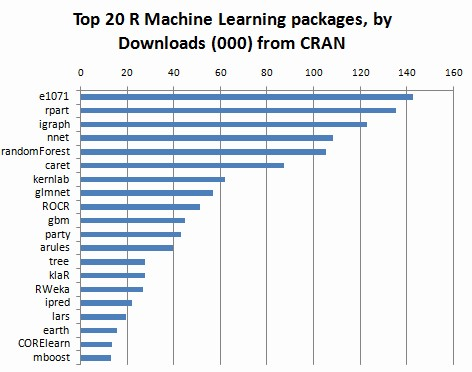
\includegraphics{top20rpkg.jpg}
\caption{Top 20 R Machine Learning and Data Science packages. From \href{http://www.kdnuggets.com/2015/06/top-20-r-machine-learning-packages.html}{http://www.kdnuggets.com/2015/06/top-20-r-machine-learning-packages.html}}\end{figure}
\end{quote}
\begin{itemize}
\item {} 
\textbf{Installing package for Python}

\end{itemize}
\begin{quote}

Install package or modules for Python in Linux can also be quite easy. Here I will only present installation by using pip.
\begin{itemize}
\item {} 
\textbf{Installing pip}

\end{itemize}
\begin{quote}

\begin{Verbatim}[commandchars=\\\{\}]
sudo easy\PYGZus{}install pip
\end{Verbatim}
\end{quote}
\begin{itemize}
\item {} 
\textbf{Installing numpy}

\end{itemize}
\begin{quote}

\begin{Verbatim}[commandchars=\\\{\}]
pip install numpy
\end{Verbatim}
\end{quote}
\begin{itemize}
\item {} 
\textbf{Installing pandas}

\end{itemize}
\begin{quote}

\begin{Verbatim}[commandchars=\\\{\}]
pip install pandas
\end{Verbatim}
\end{quote}
\begin{itemize}
\item {} 
\textbf{Installing scikits-learn}

\end{itemize}
\begin{quote}

\begin{Verbatim}[commandchars=\\\{\}]
pip install \PYGZhy{}U scikit\PYGZhy{}learn
\end{Verbatim}
\end{quote}
\end{quote}

The following are the best Python modules for data mining from \href{http://www.kdnuggets.com/2012/11/best-python-modules-for-data-mining.html}{kdnuggets}, you may also want to install all of them.
\begin{enumerate}
\item {} 
Basics

\end{enumerate}
\begin{itemize}
\item {} 
\textbf{numpy} - numerical library, \href{http://numpy.scipy.org/}{http://numpy.scipy.org/}

\item {} 
\textbf{scipy} - Advanced math, signal processing, optimization, statistics, \href{http://www.scipy.org/}{http://www.scipy.org/}

\item {} 
\textbf{matplotlib}, python plotting - Matplotlib, \href{http://matplotlib.org}{http://matplotlib.org}

\end{itemize}
\begin{enumerate}
\setcounter{enumi}{1}
\item {} 
Machine Learning and Data Mining

\end{enumerate}
\begin{itemize}
\item {} 
\textbf{MDP}, a collection of supervised and unsupervised learning algorithms, \href{http://pypi.python.org/pypi/MDP/2.4}{http://pypi.python.org/pypi/MDP/2.4}

\item {} 
\textbf{mlpy}, Machine Learning Python, \href{http://mlpy.sourceforge.net}{http://mlpy.sourceforge.net}

\item {} 
\textbf{NetworkX}, for graph analysis, \href{http://networkx.lanl.gov/}{http://networkx.lanl.gov/}

\item {} 
\textbf{Orange}, Data Mining Fruitful \& Fun, \href{http://biolab.si}{http://biolab.si}

\item {} 
\textbf{pandas}, Python Data Analysis Library, \href{http://pandas.pydata.org}{http://pandas.pydata.org}

\item {} 
\textbf{pybrain}, \href{http://pybrain.org}{http://pybrain.org}

\item {} 
\textbf{scikits-learn} - Classic machine learning algorithms - Provide simple an efficient solutions to learning problems, \href{http://scikit-learn.org/stable/}{http://scikit-learn.org/stable/}

\end{itemize}
\begin{enumerate}
\setcounter{enumi}{2}
\item {} 
Natural Language

\end{enumerate}
\begin{itemize}
\item {} 
\textbf{NLTK}, Natural Language Toolkit, \href{http://nltk.org}{http://nltk.org}

\end{itemize}
\begin{enumerate}
\setcounter{enumi}{3}
\item {} 
For web scraping

\end{enumerate}
\begin{itemize}
\item {} 
\textbf{Scrapy}, An open source web scraping framework for Python, \href{http://scrapy.org}{http://scrapy.org}

\item {} 
\textbf{urllib/urllib2}

\end{itemize}

Herein I would like to add one more important package \textbf{Theano} for deep learning and \textbf{textmining} for text mining:
\begin{quote}
\begin{itemize}
\item {} 
\textbf{Theano}, deep learning, \href{http://deeplearning.net/tutorial/}{http://deeplearning.net/tutorial/}

\item {} 
\textbf{textmining}, text mining, \href{https://pypi.python.org/pypi/textmining/1.0}{https://pypi.python.org/pypi/textmining/1.0}

\end{itemize}
\end{quote}
\phantomsection\label{dap:dap}
\index{Data analysis procedures}

\chapter{Data analysis procedures}
\label{dap:index-0}\label{dap:data-analysis-procedures}\label{dap::doc}
\begin{notice}{note}{Note:}
\textbf{Know yourself and know your enemy, and you will never be defeated} -- idiom, from Sunzi's Art of War
\end{notice}

\index{procedures}

\section{procedures}
\label{dap:procedures}\label{dap:index-1}
Data mining is a complex process that aims to discover patterns in large data sets starting from a collection of exsting data. In my opinion, data minig contains four main steps:
\begin{enumerate}
\item {} 
\textbf{Collecting data}: This is a complex step, I will assume we have already gotten the datasets.

\item {} 
\textbf{Pre-processing}: In this step, we need to try to understand your data, denoise, do dimentation reduction and select proper predictors etc.

\item {} 
\textbf{Feeding data mining}: In this step, we need to use your data to feed your model.

\item {} 
\textbf{Post-processing} : In this step, we need to interpret and evaluate your model.

\end{enumerate}

In this section, we will try to know our enemy -- datasets. We will learn how to load data, how to understand data with statistics method and how to underdtand data with visualization. Next, we will start with Loading Datasets for the Pre-processing.

\index{Datasets}

\section{Datasets in this Tutorial}
\label{dap:datasets-in-this-tutorial}\label{dap:index-2}
The datasets for this tutorial are available to download: Heart,  Energy Efficienency. Those data are from my course matrials, the copyrights blongs to the origial authors.

\index{Loading Datasets}

\section{Loading Datasets}
\label{dap:loading-datasets}\label{dap:index-3}
There are two main data formats ``\emph{.csv'' and ``}.xlsx''. We will show how to load those two types of data in \textbf{R} and \textbf{Python}, respectively.
\begin{enumerate}
\item {} 
\textbf{Loading datasets in R}

\end{enumerate}
\begin{quote}
\begin{itemize}
\item {} 
Loading \(*.csv\) format data

\end{itemize}
\begin{quote}

\begin{Verbatim}[commandchars=\\\{\}]
\PYG{c+c1}{\PYGZsh{} set the path or enverionment}
setwd\PYG{p}{(}\PYG{l+s}{\PYGZdq{}}\PYG{l+s}{/home/feng/R\PYGZhy{}language/sat577/HW\PYGZsh{}4/data\PYGZdq{}}\PYG{p}{)}

\PYG{c+c1}{\PYGZsh{} read data set}
rawdata \PYG{o}{=} read.csv\PYG{p}{(}\PYG{l+s}{\PYGZdq{}}\PYG{l+s}{spam.csv\PYGZdq{}}\PYG{p}{)}
\end{Verbatim}
\end{quote}
\begin{itemize}
\item {} 
Loading \(*.xlsx\) format data

\end{itemize}
\begin{quote}

\begin{Verbatim}[commandchars=\\\{\}]
\PYG{c+c1}{\PYGZsh{} set the path or enverionment}
setwd\PYG{p}{(}\PYG{l+s}{\PYGZdq{}}\PYG{l+s}{\PYGZti{}/Dropbox/R\PYGZhy{}language/sat577/\PYGZdq{}}\PYG{p}{)}

\PYG{c+c1}{\PYGZsh{}install.packages(\PYGZdq{}readxl\PYGZdq{}) \PYGZsh{} CRAN version}
library\PYG{p}{(}readxl\PYG{p}{)}

\PYG{c+c1}{\PYGZsh{} read data set}
energy\PYGZus{}eff\PYG{o}{=}read\PYGZus{}excel\PYG{p}{(}\PYG{l+s}{\PYGZdq{}}\PYG{l+s}{energy\PYGZus{}efficiency.xlsx\PYGZdq{}}\PYG{p}{)}
\end{Verbatim}
\end{quote}
\end{quote}
\begin{enumerate}
\setcounter{enumi}{1}
\item {} 
\textbf{Loading datasets in Python}

\end{enumerate}
\begin{quote}
\begin{itemize}
\item {} 
Loading \(*.csv\) format data

\end{itemize}
\begin{quote}

\begin{Verbatim}[commandchars=\\\{\}]
\PYG{k+kn}{import} \PYG{n+nn}{pandas} \PYG{k+kn}{as} \PYG{n+nn}{pd}

\PYG{c}{\PYGZsh{} set data path}
\PYG{n}{path} \PYG{o}{=}\PYG{l+s}{\PYGZsq{}}\PYG{l+s}{\PYGZti{}/Dropbox/MachineLearningAlgorithms/python\PYGZus{}code/data/Heart.csv}\PYG{l+s}{\PYGZsq{}}

\PYG{c}{\PYGZsh{} read data set}
\PYG{n}{rawdata} \PYG{o}{=} \PYG{n}{pd}\PYG{o}{.}\PYG{n}{read\PYGZus{}csv}\PYG{p}{(}\PYG{n}{path}\PYG{p}{)}
\end{Verbatim}
\end{quote}
\begin{itemize}
\item {} 
Loading \(*.xlsx\) format data

\end{itemize}
\begin{quote}

\begin{Verbatim}[commandchars=\\\{\}]
\PYG{k+kn}{import} \PYG{n+nn}{pandas} \PYG{k+kn}{as} \PYG{n+nn}{pd}

\PYG{c}{\PYGZsh{} set data path}
\PYG{n}{path} \PYG{o}{=} \PYG{p}{(}\PYG{l+s}{\PYGZsq{}}\PYG{l+s}{/home/feng/Dropbox/MachineLearningAlgorithms/python\PYGZus{}code/data/}\PYG{l+s}{\PYGZsq{}}
\PYG{l+s}{\PYGZsq{}}\PYG{l+s}{energy\PYGZus{}efficiency.xlsx}\PYG{l+s}{\PYGZsq{}}\PYG{p}{)}

\PYG{c}{\PYGZsh{} read data set from first sheet}
\PYG{n}{rawdata}\PYG{o}{=} \PYG{n}{pd}\PYG{o}{.}\PYG{n}{read\PYGZus{}excel}\PYG{p}{(}\PYG{n}{path}\PYG{p}{,}\PYG{n}{sheetname}\PYG{o}{=}\PYG{l+m+mi}{0}\PYG{p}{)}
\end{Verbatim}
\end{quote}
\end{quote}

\index{Understand Data With Statistics methods}

\section{Understand Data With Statistics methods}
\label{dap:index-4}\label{dap:understand-data-with-statistics-methods}
After we get the data in hand, then we can try to understand them.  I will use ``Heart.csv'' dataset as a example to demonstrate how to use those statistics methods.
\begin{enumerate}
\item {} 
\textbf{Summary of the data}

\end{enumerate}
\begin{quote}

It is always good to have a glance over the summary of the data. Since from the summary you will know some statistics features of your data, and you will also know whether you data contains missing data or not.
\begin{itemize}
\item {} 
Summary of the data in \textbf{R}

\end{itemize}
\begin{quote}

\begin{Verbatim}[commandchars=\\\{\}]
summary\PYG{p}{(}rawdata\PYG{p}{)}
\end{Verbatim}

Then you will get

\begin{Verbatim}[commandchars=\\\{\}]
\PYG{o}{\PYGZgt{}} summary\PYG{p}{(}rawdata\PYG{p}{)}
        Age             Sex                ChestPain       RestBP
     Min.   \PYG{o}{:}\PYG{l+m}{29.00}   Min.   \PYG{o}{:}\PYG{l+m}{0.0000}   asymptomatic\PYG{o}{:}\PYG{l+m}{144}   Min.   \PYG{o}{:} \PYG{l+m}{94.0}
     \PYG{l+m}{1}st Qu.\PYG{o}{:}\PYG{l+m}{48.00}   \PYG{l+m}{1}st Qu.\PYG{o}{:}\PYG{l+m}{0.0000}   nonanginal  \PYG{o}{:} \PYG{l+m}{86}   \PYG{l+m}{1}st Qu.\PYG{o}{:}\PYG{l+m}{120.0}
     Median \PYG{o}{:}\PYG{l+m}{56.00}   Median \PYG{o}{:}\PYG{l+m}{1.0000}   nontypical  \PYG{o}{:} \PYG{l+m}{50}   Median \PYG{o}{:}\PYG{l+m}{130.0}
     Mean   \PYG{o}{:}\PYG{l+m}{54.44}   Mean   \PYG{o}{:}\PYG{l+m}{0.6799}   typical     \PYG{o}{:} \PYG{l+m}{23}   Mean   \PYG{o}{:}\PYG{l+m}{131.7}
     \PYG{l+m}{3}rd Qu.\PYG{o}{:}\PYG{l+m}{61.00}   \PYG{l+m}{3}rd Qu.\PYG{o}{:}\PYG{l+m}{1.0000}                      \PYG{l+m}{3}rd Qu.\PYG{o}{:}\PYG{l+m}{140.0}
     Max.   \PYG{o}{:}\PYG{l+m}{77.00}   Max.   \PYG{o}{:}\PYG{l+m}{1.0000}                      Max.   \PYG{o}{:}\PYG{l+m}{200.0}

       Chol            Fbs            RestECG           MaxHR
     Min.   \PYG{o}{:}\PYG{l+m}{126.0}   Min.   \PYG{o}{:}\PYG{l+m}{0.0000}   Min.   \PYG{o}{:}\PYG{l+m}{0.0000}   Min.   \PYG{o}{:} \PYG{l+m}{71.0}
     \PYG{l+m}{1}st Qu.\PYG{o}{:}\PYG{l+m}{211.0}   \PYG{l+m}{1}st Qu.\PYG{o}{:}\PYG{l+m}{0.0000}   \PYG{l+m}{1}st Qu.\PYG{o}{:}\PYG{l+m}{0.0000}   \PYG{l+m}{1}st Qu.\PYG{o}{:}\PYG{l+m}{133.5}
     Median \PYG{o}{:}\PYG{l+m}{241.0}   Median \PYG{o}{:}\PYG{l+m}{0.0000}   Median \PYG{o}{:}\PYG{l+m}{1.0000}   Median \PYG{o}{:}\PYG{l+m}{153.0}
     Mean   \PYG{o}{:}\PYG{l+m}{246.7}   Mean   \PYG{o}{:}\PYG{l+m}{0.1485}   Mean   \PYG{o}{:}\PYG{l+m}{0.9901}   Mean   \PYG{o}{:}\PYG{l+m}{149.6}
     \PYG{l+m}{3}rd Qu.\PYG{o}{:}\PYG{l+m}{275.0}   \PYG{l+m}{3}rd Qu.\PYG{o}{:}\PYG{l+m}{0.0000}   \PYG{l+m}{3}rd Qu.\PYG{o}{:}\PYG{l+m}{2.0000}   \PYG{l+m}{3}rd Qu.\PYG{o}{:}\PYG{l+m}{166.0}
     Max.   \PYG{o}{:}\PYG{l+m}{564.0}   Max.   \PYG{o}{:}\PYG{l+m}{1.0000}   Max.   \PYG{o}{:}\PYG{l+m}{2.0000}   Max.   \PYG{o}{:}\PYG{l+m}{202.0}

      ExAng           Oldpeak         Slope             Ca
     Min.   \PYG{o}{:}\PYG{l+m}{0.0000}   Min.   \PYG{o}{:}\PYG{l+m}{0.00}   Min.   \PYG{o}{:}\PYG{l+m}{1.000}   Min.   \PYG{o}{:}\PYG{l+m}{0.0000}
     \PYG{l+m}{1}st Qu.\PYG{o}{:}\PYG{l+m}{0.0000}   \PYG{l+m}{1}st Qu.\PYG{o}{:}\PYG{l+m}{0.00}   \PYG{l+m}{1}st Qu.\PYG{o}{:}\PYG{l+m}{1.000}   \PYG{l+m}{1}st Qu.\PYG{o}{:}\PYG{l+m}{0.0000}
     Median \PYG{o}{:}\PYG{l+m}{0.0000}   Median \PYG{o}{:}\PYG{l+m}{0.80}   Median \PYG{o}{:}\PYG{l+m}{2.000}   Median \PYG{o}{:}\PYG{l+m}{0.0000}
     Mean   \PYG{o}{:}\PYG{l+m}{0.3267}   Mean   \PYG{o}{:}\PYG{l+m}{1.04}   Mean   \PYG{o}{:}\PYG{l+m}{1.601}   Mean   \PYG{o}{:}\PYG{l+m}{0.6722}
     \PYG{l+m}{3}rd Qu.\PYG{o}{:}\PYG{l+m}{1.0000}   \PYG{l+m}{3}rd Qu.\PYG{o}{:}\PYG{l+m}{1.60}   \PYG{l+m}{3}rd Qu.\PYG{o}{:}\PYG{l+m}{2.000}   \PYG{l+m}{3}rd Qu.\PYG{o}{:}\PYG{l+m}{1.0000}
     Max.   \PYG{o}{:}\PYG{l+m}{1.0000}   Max.   \PYG{o}{:}\PYG{l+m}{6.20}   Max.   \PYG{o}{:}\PYG{l+m}{3.000}   Max.   \PYG{o}{:}\PYG{l+m}{3.0000}
                                             \PYG{k+kc}{NA}\PYG{l+s}{\PYGZsq{}}\PYG{l+s}{s   :4}
\PYG{l+s}{         Thal      AHD}
\PYG{l+s}{     fixed     : 18   No :164}
\PYG{l+s}{     normal    :166   Yes:139}
\PYG{l+s}{     reversable:117}
\PYG{l+s}{     NA\PYGZsq{}}s      \PYG{o}{:}  \PYG{l+m}{2}
\end{Verbatim}
\end{quote}
\begin{itemize}
\item {} 
Summary of the data in \textbf{Python}

\end{itemize}
\begin{quote}

\begin{Verbatim}[commandchars=\\\{\}]
\PYG{k}{print} \PYG{l+s}{\PYGZdq{}}\PYG{l+s}{data summary}\PYG{l+s}{\PYGZdq{}}
\PYG{k}{print} \PYG{n}{rawdata}\PYG{o}{.}\PYG{n}{describe}\PYG{p}{(}\PYG{p}{)}
\end{Verbatim}

Then you will get

\begin{Verbatim}[commandchars=\\\{\}]
              \PYG{n}{Age}         \PYG{n}{Sex}      \PYG{n}{RestBP}        \PYG{n}{Chol}         \PYG{n}{Fbs}     \PYG{n}{RestECG}  \PYGZbs{}
\PYG{n}{count}  \PYG{l+m+mf}{303.000000}  \PYG{l+m+mf}{303.000000}  \PYG{l+m+mf}{303.000000}  \PYG{l+m+mf}{303.000000}  \PYG{l+m+mf}{303.000000}  \PYG{l+m+mf}{303.000000}
\PYG{n}{mean}    \PYG{l+m+mf}{54.438944}    \PYG{l+m+mf}{0.679868}  \PYG{l+m+mf}{131.689769}  \PYG{l+m+mf}{246.693069}    \PYG{l+m+mf}{0.148515}    \PYG{l+m+mf}{0.990099}
\PYG{n}{std}      \PYG{l+m+mf}{9.038662}    \PYG{l+m+mf}{0.467299}   \PYG{l+m+mf}{17.599748}   \PYG{l+m+mf}{51.776918}    \PYG{l+m+mf}{0.356198}    \PYG{l+m+mf}{0.994971}
\PYG{n+nb}{min}     \PYG{l+m+mf}{29.000000}    \PYG{l+m+mf}{0.000000}   \PYG{l+m+mf}{94.000000}  \PYG{l+m+mf}{126.000000}    \PYG{l+m+mf}{0.000000}    \PYG{l+m+mf}{0.000000}
\PYG{l+m+mi}{25}\PYG{o}{\PYGZpc{}}     \PYG{l+m+mf}{48.000000}    \PYG{l+m+mf}{0.000000}  \PYG{l+m+mf}{120.000000}  \PYG{l+m+mf}{211.000000}    \PYG{l+m+mf}{0.000000}    \PYG{l+m+mf}{0.000000}
\PYG{l+m+mi}{50}\PYG{o}{\PYGZpc{}}     \PYG{l+m+mf}{56.000000}    \PYG{l+m+mf}{1.000000}  \PYG{l+m+mf}{130.000000}  \PYG{l+m+mf}{241.000000}    \PYG{l+m+mf}{0.000000}    \PYG{l+m+mf}{1.000000}
\PYG{l+m+mi}{75}\PYG{o}{\PYGZpc{}}     \PYG{l+m+mf}{61.000000}    \PYG{l+m+mf}{1.000000}  \PYG{l+m+mf}{140.000000}  \PYG{l+m+mf}{275.000000}    \PYG{l+m+mf}{0.000000}    \PYG{l+m+mf}{2.000000}
\PYG{n+nb}{max}     \PYG{l+m+mf}{77.000000}    \PYG{l+m+mf}{1.000000}  \PYG{l+m+mf}{200.000000}  \PYG{l+m+mf}{564.000000}    \PYG{l+m+mf}{1.000000}    \PYG{l+m+mf}{2.000000}

       \PYG{n}{MaxHR}       \PYG{n}{ExAng}     \PYG{n}{Oldpeak}       \PYG{n}{Slope}          \PYG{n}{Ca}
\PYG{n}{count}  \PYG{l+m+mf}{303.000000}  \PYG{l+m+mf}{303.000000}  \PYG{l+m+mf}{303.000000}  \PYG{l+m+mf}{303.000000}  \PYG{l+m+mf}{299.000000}
\PYG{n}{mean}   \PYG{l+m+mf}{149.607261}    \PYG{l+m+mf}{0.326733}    \PYG{l+m+mf}{1.039604}    \PYG{l+m+mf}{1.600660}    \PYG{l+m+mf}{0.672241}
\PYG{n}{std}     \PYG{l+m+mf}{22.875003}    \PYG{l+m+mf}{0.469794}    \PYG{l+m+mf}{1.161075}    \PYG{l+m+mf}{0.616226}    \PYG{l+m+mf}{0.937438}
\PYG{n+nb}{min}     \PYG{l+m+mf}{71.000000}    \PYG{l+m+mf}{0.000000}    \PYG{l+m+mf}{0.000000}    \PYG{l+m+mf}{1.000000}    \PYG{l+m+mf}{0.000000}
\PYG{l+m+mi}{25}\PYG{o}{\PYGZpc{}}    \PYG{l+m+mf}{133.500000}    \PYG{l+m+mf}{0.000000}    \PYG{l+m+mf}{0.000000}    \PYG{l+m+mf}{1.000000}    \PYG{l+m+mf}{0.000000}
\PYG{l+m+mi}{50}\PYG{o}{\PYGZpc{}}    \PYG{l+m+mf}{153.000000}    \PYG{l+m+mf}{0.000000}    \PYG{l+m+mf}{0.800000}    \PYG{l+m+mf}{2.000000}    \PYG{l+m+mf}{0.000000}
\PYG{l+m+mi}{75}\PYG{o}{\PYGZpc{}}    \PYG{l+m+mf}{166.000000}    \PYG{l+m+mf}{1.000000}    \PYG{l+m+mf}{1.600000}    \PYG{l+m+mf}{2.000000}    \PYG{l+m+mf}{1.000000}
\PYG{n+nb}{max}    \PYG{l+m+mf}{202.000000}    \PYG{l+m+mf}{1.000000}    \PYG{l+m+mf}{6.200000}    \PYG{l+m+mf}{3.000000}    \PYG{l+m+mf}{3.000000}
\end{Verbatim}
\end{quote}
\end{quote}
\begin{enumerate}
\setcounter{enumi}{1}
\item {} 
\textbf{The size of the data}

\end{enumerate}
\begin{quote}

Sometimes we also need to know the size or dimension of our data. Such as when you need to extract the
response from the dataset, you need the number of column, or when you try to split your data into train
and test data set, you need know the number of row.
\begin{itemize}
\item {} 
Checking size in \textbf{R}

\end{itemize}
\begin{quote}

\begin{Verbatim}[commandchars=\\\{\}]
dim\PYG{p}{(}rawdata\PYG{p}{)}
\end{Verbatim}

Or you can use the following code

\begin{Verbatim}[commandchars=\\\{\}]
nrow\PYG{o}{=}nrow\PYG{p}{(}rawdata\PYG{p}{)}
ncol\PYG{o}{=}ncol\PYG{p}{(}rawdata\PYG{p}{)}

c\PYG{p}{(}nrow\PYG{p}{,} ncol\PYG{p}{)}
\end{Verbatim}

Then you will get

\begin{Verbatim}[commandchars=\\\{\}]
\PYG{o}{\PYGZgt{}} dim\PYG{p}{(}rawdata\PYG{p}{)}
\PYG{p}{[}\PYG{l+m}{1}\PYG{p}{]} \PYG{l+m}{303}  \PYG{l+m}{14}
\end{Verbatim}
\end{quote}
\begin{itemize}
\item {} 
Checking size in \textbf{Python}

\end{itemize}
\begin{quote}

\begin{Verbatim}[commandchars=\\\{\}]
\PYG{n}{nrow}\PYG{p}{,} \PYG{n}{ncol} \PYG{o}{=} \PYG{n}{rawdata}\PYG{o}{.}\PYG{n}{shape}
\PYG{k}{print} \PYG{n}{nrow}\PYG{p}{,} \PYG{n}{ncol}
\end{Verbatim}

or you can use the follwing code

\begin{Verbatim}[commandchars=\\\{\}]
\PYG{n}{nrow}\PYG{o}{=}\PYG{n}{rawdata}\PYG{o}{.}\PYG{n}{shape}\PYG{p}{[}\PYG{l+m+mi}{0}\PYG{p}{]} \PYG{c}{\PYGZsh{}gives number of row count}
\PYG{n}{ncol}\PYG{o}{=}\PYG{n}{rawdata}\PYG{o}{.}\PYG{n}{shape}\PYG{p}{[}\PYG{l+m+mi}{1}\PYG{p}{]} \PYG{c}{\PYGZsh{}gives number of col count}
\PYG{k}{print} \PYG{n}{nrow}\PYG{p}{,} \PYG{n}{ncol}
\end{Verbatim}

Then you will get

\begin{Verbatim}[commandchars=\\\{\}]
\PYG{n}{Raw} \PYG{n}{data} \PYG{n}{size}
\PYG{l+m+mi}{303} \PYG{l+m+mi}{14}
\end{Verbatim}
\end{quote}
\end{quote}
\begin{enumerate}
\setcounter{enumi}{2}
\item {} 
\textbf{Data format of the predictors}

\end{enumerate}
\begin{quote}

Data format is also very important, since some functions or methods can not be applied to the qualitative data, you
need to remove those predictors or transform them into quantitative data.
\begin{itemize}
\item {} 
Checking data format in \textbf{R}

\end{itemize}
\begin{quote}

\begin{Verbatim}[commandchars=\\\{\}]
\PYG{c+c1}{\PYGZsh{} install the package}
install.packages\PYG{p}{(}\PYG{l+s}{\PYGZdq{}}\PYG{l+s}{mlbench\PYGZdq{}}\PYG{p}{)}
library\PYG{p}{(}mlbench\PYG{p}{)}

sapply\PYG{p}{(}rawdata\PYG{p}{,} class\PYG{p}{)}
\end{Verbatim}

Then you will get

\begin{Verbatim}[commandchars=\\\{\}]
   \PYG{o}{\PYGZgt{}} sapply\PYG{p}{(}rawdata\PYG{p}{,} class\PYG{p}{)}
    Age       Sex ChestPain    RestBP      Chol       Fbs   RestECG
\PYG{l+s}{\PYGZdq{}}\PYG{l+s}{integer\PYGZdq{}} \PYG{l+s}{\PYGZdq{}}\PYG{l+s}{integer\PYGZdq{}}  \PYG{l+s}{\PYGZdq{}}\PYG{l+s}{factor\PYGZdq{}} \PYG{l+s}{\PYGZdq{}}\PYG{l+s}{integer\PYGZdq{}} \PYG{l+s}{\PYGZdq{}}\PYG{l+s}{integer\PYGZdq{}} \PYG{l+s}{\PYGZdq{}}\PYG{l+s}{integer\PYGZdq{}} \PYG{l+s}{\PYGZdq{}}\PYG{l+s}{integer\PYGZdq{}}
MaxHR     ExAng   Oldpeak     Slope        Ca      Thal       AHD
\PYG{l+s}{\PYGZdq{}}\PYG{l+s}{integer\PYGZdq{}} \PYG{l+s}{\PYGZdq{}}\PYG{l+s}{integer\PYGZdq{}} \PYG{l+s}{\PYGZdq{}}\PYG{l+s}{numeric\PYGZdq{}} \PYG{l+s}{\PYGZdq{}}\PYG{l+s}{integer\PYGZdq{}} \PYG{l+s}{\PYGZdq{}}\PYG{l+s}{integer\PYGZdq{}}  \PYG{l+s}{\PYGZdq{}}\PYG{l+s}{factor\PYGZdq{}}  \PYG{l+s}{\PYGZdq{}}\PYG{l+s}{factor\PYGZdq{}}
\end{Verbatim}
\end{quote}
\begin{itemize}
\item {} 
Checking data format in \textbf{Pyhton}

\end{itemize}
\begin{quote}

\begin{Verbatim}[commandchars=\\\{\}]
\PYG{k}{print} \PYG{n}{rawdata}\PYG{o}{.}\PYG{n}{dtypes}
\end{Verbatim}

Then you will get

\begin{Verbatim}[commandchars=\\\{\}]
\PYG{n}{Data} \PYG{n}{Format}\PYG{p}{:}
\PYG{n}{Age}            \PYG{n}{int64}
\PYG{n}{Sex}            \PYG{n}{int64}
\PYG{n}{ChestPain}     \PYG{n+nb}{object}
\PYG{n}{RestBP}         \PYG{n}{int64}
\PYG{n}{Chol}           \PYG{n}{int64}
\PYG{n}{Fbs}            \PYG{n}{int64}
\PYG{n}{RestECG}        \PYG{n}{int64}
\PYG{n}{MaxHR}          \PYG{n}{int64}
\PYG{n}{ExAng}          \PYG{n}{int64}
\PYG{n}{Oldpeak}      \PYG{n}{float64}
\PYG{n}{Slope}          \PYG{n}{int64}
\PYG{n}{Ca}           \PYG{n}{float64}
\PYG{n}{Thal}          \PYG{n+nb}{object}
\PYG{n}{AHD}           \PYG{n+nb}{object}
\PYG{n}{dtype}\PYG{p}{:} \PYG{n+nb}{object}
\end{Verbatim}
\end{quote}
\end{quote}
\begin{enumerate}
\setcounter{enumi}{3}
\item {} 
\textbf{The column names}

\end{enumerate}
\begin{quote}
\begin{itemize}
\item {} 
Checking column names of the data in \textbf{R}

\end{itemize}
\begin{quote}

\begin{Verbatim}[commandchars=\\\{\}]
colnames\PYG{p}{(}rawdata\PYG{p}{)}
attach\PYG{p}{(}rawdata\PYG{p}{)} \PYG{c+c1}{\PYGZsh{} enable you can directly use name as predictors}
\end{Verbatim}

Then you will get

\begin{Verbatim}[commandchars=\\\{\}]
   \PYG{o}{\PYGZgt{}} colnames\PYG{p}{(}rawdata\PYG{p}{)}
\PYG{p}{[}\PYG{l+m}{1}\PYG{p}{]} \PYG{l+s}{\PYGZdq{}}\PYG{l+s}{Age\PYGZdq{}}       \PYG{l+s}{\PYGZdq{}}\PYG{l+s}{Sex\PYGZdq{}}       \PYG{l+s}{\PYGZdq{}}\PYG{l+s}{ChestPain\PYGZdq{}} \PYG{l+s}{\PYGZdq{}}\PYG{l+s}{RestBP\PYGZdq{}}    \PYG{l+s}{\PYGZdq{}}\PYG{l+s}{Chol\PYGZdq{}}
\PYG{p}{[}\PYG{l+m}{6}\PYG{p}{]} \PYG{l+s}{\PYGZdq{}}\PYG{l+s}{Fbs\PYGZdq{}}       \PYG{l+s}{\PYGZdq{}}\PYG{l+s}{RestECG\PYGZdq{}}   \PYG{l+s}{\PYGZdq{}}\PYG{l+s}{MaxHR\PYGZdq{}}     \PYG{l+s}{\PYGZdq{}}\PYG{l+s}{ExAng\PYGZdq{}}     \PYG{l+s}{\PYGZdq{}}\PYG{l+s}{Oldpeak\PYGZdq{}}
\PYG{p}{[}\PYG{l+m}{11}\PYG{p}{]} \PYG{l+s}{\PYGZdq{}}\PYG{l+s}{Slope\PYGZdq{}}     \PYG{l+s}{\PYGZdq{}}\PYG{l+s}{Ca\PYGZdq{}}        \PYG{l+s}{\PYGZdq{}}\PYG{l+s}{Thal\PYGZdq{}}      \PYG{l+s}{\PYGZdq{}}\PYG{l+s}{AHD\PYGZdq{}}
\end{Verbatim}
\end{quote}
\begin{itemize}
\item {} 
Checking column names of the data in \textbf{Python}

\end{itemize}
\begin{quote}

\begin{Verbatim}[commandchars=\\\{\}]
\PYG{n}{colNames} \PYG{o}{=} \PYG{n}{rawdata}\PYG{o}{.}\PYG{n}{columns}\PYG{o}{.}\PYG{n}{tolist}\PYG{p}{(}\PYG{p}{)}

\PYG{k}{print} \PYG{l+s}{\PYGZdq{}}\PYG{l+s}{Column names:}\PYG{l+s}{\PYGZdq{}}
\PYG{k}{print} \PYG{n}{colNames}
\end{Verbatim}

Then you will get

\begin{Verbatim}[commandchars=\\\{\}]
    \PYG{n}{Column} \PYG{n}{names}\PYG{p}{:}
\PYG{p}{[}\PYG{l+s}{\PYGZsq{}}\PYG{l+s}{Age}\PYG{l+s}{\PYGZsq{}}\PYG{p}{,} \PYG{l+s}{\PYGZsq{}}\PYG{l+s}{Sex}\PYG{l+s}{\PYGZsq{}}\PYG{p}{,} \PYG{l+s}{\PYGZsq{}}\PYG{l+s}{ChestPain}\PYG{l+s}{\PYGZsq{}}\PYG{p}{,} \PYG{l+s}{\PYGZsq{}}\PYG{l+s}{RestBP}\PYG{l+s}{\PYGZsq{}}\PYG{p}{,} \PYG{l+s}{\PYGZsq{}}\PYG{l+s}{Chol}\PYG{l+s}{\PYGZsq{}}\PYG{p}{,} \PYG{l+s}{\PYGZsq{}}\PYG{l+s}{Fbs}\PYG{l+s}{\PYGZsq{}}\PYG{p}{,} \PYG{l+s}{\PYGZsq{}}\PYG{l+s}{RestECG}\PYG{l+s}{\PYGZsq{}}\PYG{p}{,} \PYG{l+s}{\PYGZsq{}}\PYG{l+s}{MaxHR}\PYG{l+s}{\PYGZsq{}}\PYG{p}{,}
 \PYG{l+s}{\PYGZsq{}}\PYG{l+s}{ExAng}\PYG{l+s}{\PYGZsq{}}\PYG{p}{,} \PYG{l+s}{\PYGZsq{}}\PYG{l+s}{Oldpeak}\PYG{l+s}{\PYGZsq{}}\PYG{p}{,} \PYG{l+s}{\PYGZsq{}}\PYG{l+s}{Slope}\PYG{l+s}{\PYGZsq{}}\PYG{p}{,} \PYG{l+s}{\PYGZsq{}}\PYG{l+s}{Ca}\PYG{l+s}{\PYGZsq{}}\PYG{p}{,} \PYG{l+s}{\PYGZsq{}}\PYG{l+s}{Thal}\PYG{l+s}{\PYGZsq{}}\PYG{p}{,} \PYG{l+s}{\PYGZsq{}}\PYG{l+s}{AHD}\PYG{l+s}{\PYGZsq{}}\PYG{p}{]}
\end{Verbatim}
\end{quote}
\end{quote}
\begin{enumerate}
\setcounter{enumi}{4}
\item {} 
\textbf{The first or last parts of the data}

\end{enumerate}
\begin{quote}
\begin{itemize}
\item {} 
Checking first parts of the data in \textbf{R}

\end{itemize}
\begin{quote}

\begin{Verbatim}[commandchars=\\\{\}]
head\PYG{p}{(}rawdata\PYG{p}{)}
\end{Verbatim}

Then you will get

\begin{Verbatim}[commandchars=\\\{\}]
\PYG{o}{\PYGZgt{}} head\PYG{p}{(}rawdata\PYG{p}{)}
   Age Sex    ChestPain RestBP Chol Fbs RestECG MaxHR ExAng Oldpeak
 \PYG{l+m}{1}  \PYG{l+m}{63}   \PYG{l+m}{1}      typical    \PYG{l+m}{145}  \PYG{l+m}{233}   \PYG{l+m}{1}       \PYG{l+m}{2}   \PYG{l+m}{150}     \PYG{l+m}{0}     \PYG{l+m}{2.3}
 \PYG{l+m}{2}  \PYG{l+m}{67}   \PYG{l+m}{1} asymptomatic    \PYG{l+m}{160}  \PYG{l+m}{286}   \PYG{l+m}{0}       \PYG{l+m}{2}   \PYG{l+m}{108}     \PYG{l+m}{1}     \PYG{l+m}{1.5}
 \PYG{l+m}{3}  \PYG{l+m}{67}   \PYG{l+m}{1} asymptomatic    \PYG{l+m}{120}  \PYG{l+m}{229}   \PYG{l+m}{0}       \PYG{l+m}{2}   \PYG{l+m}{129}     \PYG{l+m}{1}     \PYG{l+m}{2.6}
 \PYG{l+m}{4}  \PYG{l+m}{37}   \PYG{l+m}{1}   nonanginal    \PYG{l+m}{130}  \PYG{l+m}{250}   \PYG{l+m}{0}       \PYG{l+m}{0}   \PYG{l+m}{187}     \PYG{l+m}{0}     \PYG{l+m}{3.5}
 \PYG{l+m}{5}  \PYG{l+m}{41}   \PYG{l+m}{0}   nontypical    \PYG{l+m}{130}  \PYG{l+m}{204}   \PYG{l+m}{0}       \PYG{l+m}{2}   \PYG{l+m}{172}     \PYG{l+m}{0}     \PYG{l+m}{1.4}
 \PYG{l+m}{6}  \PYG{l+m}{56}   \PYG{l+m}{1}   nontypical    \PYG{l+m}{120}  \PYG{l+m}{236}   \PYG{l+m}{0}       \PYG{l+m}{0}   \PYG{l+m}{178}     \PYG{l+m}{0}     \PYG{l+m}{0.8}
    Slope Ca       Thal AHD
 \PYG{l+m}{1}     \PYG{l+m}{3}  \PYG{l+m}{0}      fixed  No
 \PYG{l+m}{2}     \PYG{l+m}{2}  \PYG{l+m}{3}     normal Yes
 \PYG{l+m}{3}     \PYG{l+m}{2}  \PYG{l+m}{2} reversable Yes
 \PYG{l+m}{4}     \PYG{l+m}{3}  \PYG{l+m}{0}     normal  No
 \PYG{l+m}{5}     \PYG{l+m}{1}  \PYG{l+m}{0}     normal  No
 \PYG{l+m}{6}     \PYG{l+m}{1}  \PYG{l+m}{0}     normal  No
\end{Verbatim}
\end{quote}
\begin{itemize}
\item {} 
Checking first parts of the data in \textbf{Python}

\end{itemize}
\begin{quote}

\begin{Verbatim}[commandchars=\\\{\}]
\PYG{k}{print} \PYG{l+s}{\PYGZdq{}}\PYG{l+s+se}{\PYGZbs{}n}\PYG{l+s}{ Sample data:}\PYG{l+s}{\PYGZdq{}}
\PYG{k}{print}\PYG{p}{(}\PYG{n}{rawdata}\PYG{o}{.}\PYG{n}{head}\PYG{p}{(}\PYG{l+m+mi}{6}\PYG{p}{)}\PYG{p}{)}
\end{Verbatim}

Then you will get

\begin{Verbatim}[commandchars=\\\{\}]
 \PYG{n}{Sample} \PYG{n}{data}\PYG{p}{:}
    \PYG{n}{Age}  \PYG{n}{Sex}     \PYG{n}{ChestPain}  \PYG{n}{RestBP}  \PYG{n}{Chol}  \PYG{n}{Fbs}  \PYG{n}{RestECG}  \PYG{n}{MaxHR}  \PYG{n}{ExAng}  \PYG{n}{Oldpeak}  \PYGZbs{}
\PYG{l+m+mi}{0}   \PYG{l+m+mi}{63}    \PYG{l+m+mi}{1}       \PYG{n}{typical}     \PYG{l+m+mi}{145}   \PYG{l+m+mi}{233}    \PYG{l+m+mi}{1}        \PYG{l+m+mi}{2}    \PYG{l+m+mi}{150}      \PYG{l+m+mi}{0}      \PYG{l+m+mf}{2.3}
\PYG{l+m+mi}{1}   \PYG{l+m+mi}{67}    \PYG{l+m+mi}{1}  \PYG{n}{asymptomatic}     \PYG{l+m+mi}{160}   \PYG{l+m+mi}{286}    \PYG{l+m+mi}{0}        \PYG{l+m+mi}{2}    \PYG{l+m+mi}{108}      \PYG{l+m+mi}{1}      \PYG{l+m+mf}{1.5}
\PYG{l+m+mi}{2}   \PYG{l+m+mi}{67}    \PYG{l+m+mi}{1}  \PYG{n}{asymptomatic}     \PYG{l+m+mi}{120}   \PYG{l+m+mi}{229}    \PYG{l+m+mi}{0}        \PYG{l+m+mi}{2}    \PYG{l+m+mi}{129}      \PYG{l+m+mi}{1}      \PYG{l+m+mf}{2.6}
\PYG{l+m+mi}{3}   \PYG{l+m+mi}{37}    \PYG{l+m+mi}{1}    \PYG{n}{nonanginal}     \PYG{l+m+mi}{130}   \PYG{l+m+mi}{250}    \PYG{l+m+mi}{0}        \PYG{l+m+mi}{0}    \PYG{l+m+mi}{187}      \PYG{l+m+mi}{0}      \PYG{l+m+mf}{3.5}
\PYG{l+m+mi}{4}   \PYG{l+m+mi}{41}    \PYG{l+m+mi}{0}    \PYG{n}{nontypical}     \PYG{l+m+mi}{130}   \PYG{l+m+mi}{204}    \PYG{l+m+mi}{0}        \PYG{l+m+mi}{2}    \PYG{l+m+mi}{172}      \PYG{l+m+mi}{0}      \PYG{l+m+mf}{1.4}
\PYG{l+m+mi}{5}   \PYG{l+m+mi}{56}    \PYG{l+m+mi}{1}    \PYG{n}{nontypical}     \PYG{l+m+mi}{120}   \PYG{l+m+mi}{236}    \PYG{l+m+mi}{0}        \PYG{l+m+mi}{0}    \PYG{l+m+mi}{178}      \PYG{l+m+mi}{0}      \PYG{l+m+mf}{0.8}

   \PYG{n}{Slope}  \PYG{n}{Ca}        \PYG{n}{Thal}  \PYG{n}{AHD}
\PYG{l+m+mi}{0}      \PYG{l+m+mi}{3}   \PYG{l+m+mi}{0}       \PYG{n}{fixed}   \PYG{n}{No}
\PYG{l+m+mi}{1}      \PYG{l+m+mi}{2}   \PYG{l+m+mi}{3}      \PYG{n}{normal}  \PYG{n}{Yes}
\PYG{l+m+mi}{2}      \PYG{l+m+mi}{2}   \PYG{l+m+mi}{2}  \PYG{n}{reversable}  \PYG{n}{Yes}
\PYG{l+m+mi}{3}      \PYG{l+m+mi}{3}   \PYG{l+m+mi}{0}      \PYG{n}{normal}   \PYG{n}{No}
\PYG{l+m+mi}{4}      \PYG{l+m+mi}{1}   \PYG{l+m+mi}{0}      \PYG{n}{normal}   \PYG{n}{No}
\PYG{l+m+mi}{5}      \PYG{l+m+mi}{1}   \PYG{l+m+mi}{0}      \PYG{n}{normal}   \PYG{n}{No}
\end{Verbatim}
\end{quote}

You can use the samilar way to check the last part of the data, for simplicity, i will skip  it.
\end{quote}
\begin{enumerate}
\setcounter{enumi}{5}
\item {} 
Correlation Matrix

\end{enumerate}
\begin{quote}
\begin{itemize}
\item {} 
Computing correlation matrix in \textbf{R}

\end{itemize}
\begin{quote}

\begin{Verbatim}[commandchars=\\\{\}]
\PYG{c+c1}{\PYGZsh{} get numerical data and remove NAN}
numdata\PYG{o}{=}na.omit\PYG{p}{(}rawdata\PYG{p}{[}\PYG{p}{,}c\PYG{p}{(}\PYG{l+m}{1}\PYG{o}{:}\PYG{l+m}{2}\PYG{p}{,}\PYG{l+m}{4}\PYG{o}{:}\PYG{l+m}{12}\PYG{p}{)}\PYG{p}{]}\PYG{p}{)}

\PYG{c+c1}{\PYGZsh{} computing correlation matrix}
cor\PYG{p}{(}numdata\PYG{p}{)}
\end{Verbatim}

Then you will get

\begin{Verbatim}[commandchars=\\\{\}]
    \PYG{o}{\PYGZgt{}} cor\PYG{p}{(}numdata\PYG{p}{)}
             Age         Sex      RestBP         Chol          Fbs
Age      \PYG{l+m}{1.00000000} \PYG{l+m}{\PYGZhy{}0.09181347}  \PYG{l+m}{0.29069633}  \PYG{l+m}{0.203376601}  \PYG{l+m}{0.128675921}
Sex     \PYG{l+m}{\PYGZhy{}0.09181347}  \PYG{l+m}{1.00000000} \PYG{l+m}{\PYGZhy{}0.06552127} \PYG{l+m}{\PYGZhy{}0.195907357}  \PYG{l+m}{0.045861783}
RestBP   \PYG{l+m}{0.29069633} \PYG{l+m}{\PYGZhy{}0.06552127}  \PYG{l+m}{1.00000000}  \PYG{l+m}{0.132284171}  \PYG{l+m}{0.177623291}
Chol     \PYG{l+m}{0.20337660} \PYG{l+m}{\PYGZhy{}0.19590736}  \PYG{l+m}{0.13228417}  \PYG{l+m}{1.000000000}  \PYG{l+m}{0.006664176}
Fbs      \PYG{l+m}{0.12867592}  \PYG{l+m}{0.04586178}  \PYG{l+m}{0.17762329}  \PYG{l+m}{0.006664176}  \PYG{l+m}{1.000000000}
RestECG  \PYG{l+m}{0.14974915}  \PYG{l+m}{0.02643577}  \PYG{l+m}{0.14870922}  \PYG{l+m}{0.164957542}  \PYG{l+m}{0.058425836}
MaxHR   \PYG{l+m}{\PYGZhy{}0.39234176} \PYG{l+m}{\PYGZhy{}0.05206445} \PYG{l+m}{\PYGZhy{}0.04805281}  \PYG{l+m}{0.002179081} \PYG{l+m}{\PYGZhy{}0.003386615}
ExAng    \PYG{l+m}{0.09510850}  \PYG{l+m}{0.14903849}  \PYG{l+m}{0.06588463}  \PYG{l+m}{0.056387955}  \PYG{l+m}{0.011636935}
Oldpeak  \PYG{l+m}{0.19737552}  \PYG{l+m}{0.11023676}  \PYG{l+m}{0.19161540}  \PYG{l+m}{0.040430535}  \PYG{l+m}{0.009092935}
Slope    \PYG{l+m}{0.15895990}  \PYG{l+m}{0.03933739}  \PYG{l+m}{0.12110773} \PYG{l+m}{\PYGZhy{}0.009008239}  \PYG{l+m}{0.053776677}
Ca       \PYG{l+m}{0.36260453}  \PYG{l+m}{0.09318476}  \PYG{l+m}{0.09877326}  \PYG{l+m}{0.119000487}  \PYG{l+m}{0.145477522}
           RestECG        MaxHR       ExAng      Oldpeak        Slope
Age      \PYG{l+m}{0.14974915} \PYG{l+m}{\PYGZhy{}0.392341763}  \PYG{l+m}{0.09510850}  \PYG{l+m}{0.197375523}  \PYG{l+m}{0.158959901}
Sex      \PYG{l+m}{0.02643577} \PYG{l+m}{\PYGZhy{}0.052064447}  \PYG{l+m}{0.14903849}  \PYG{l+m}{0.110236756}  \PYG{l+m}{0.039337394}
RestBP   \PYG{l+m}{0.14870922} \PYG{l+m}{\PYGZhy{}0.048052805}  \PYG{l+m}{0.06588463}  \PYG{l+m}{0.191615405}  \PYG{l+m}{0.121107727}
Chol     \PYG{l+m}{0.16495754}  \PYG{l+m}{0.002179081}  \PYG{l+m}{0.05638795}  \PYG{l+m}{0.040430535} \PYG{l+m}{\PYGZhy{}0.009008239}
Fbs      \PYG{l+m}{0.05842584} \PYG{l+m}{\PYGZhy{}0.003386615}  \PYG{l+m}{0.01163693}  \PYG{l+m}{0.009092935}  \PYG{l+m}{0.053776677}
RestECG  \PYG{l+m}{1.00000000} \PYG{l+m}{\PYGZhy{}0.077798148}  \PYG{l+m}{0.07408360}  \PYG{l+m}{0.110275054}  \PYG{l+m}{0.128907169}
MaxHR   \PYG{l+m}{\PYGZhy{}0.07779815}  \PYG{l+m}{1.000000000} \PYG{l+m}{\PYGZhy{}0.37635897} \PYG{l+m}{\PYGZhy{}0.341262236} \PYG{l+m}{\PYGZhy{}0.381348495}
ExAng    \PYG{l+m}{0.07408360} \PYG{l+m}{\PYGZhy{}0.376358975}  \PYG{l+m}{1.00000000}  \PYG{l+m}{0.289573103}  \PYG{l+m}{0.254302081}
Oldpeak  \PYG{l+m}{0.11027505} \PYG{l+m}{\PYGZhy{}0.341262236}  \PYG{l+m}{0.28957310}  \PYG{l+m}{1.000000000}  \PYG{l+m}{0.579775260}
Slope    \PYG{l+m}{0.12890717} \PYG{l+m}{\PYGZhy{}0.381348495}  \PYG{l+m}{0.25430208}  \PYG{l+m}{0.579775260}  \PYG{l+m}{1.000000000}
Ca       \PYG{l+m}{0.12834265} \PYG{l+m}{\PYGZhy{}0.264246253}  \PYG{l+m}{0.14556960}  \PYG{l+m}{0.295832115}  \PYG{l+m}{0.110119188}
            Ca
Age      \PYG{l+m}{0.36260453}
Sex      \PYG{l+m}{0.09318476}
RestBP   \PYG{l+m}{0.09877326}
Chol     \PYG{l+m}{0.11900049}
Fbs      \PYG{l+m}{0.14547752}
RestECG  \PYG{l+m}{0.12834265}
MaxHR   \PYG{l+m}{\PYGZhy{}0.26424625}
ExAng    \PYG{l+m}{0.14556960}
Oldpeak  \PYG{l+m}{0.29583211}
Slope    \PYG{l+m}{0.11011919}
Ca       \PYG{l+m}{1.00000000}
\end{Verbatim}
\end{quote}
\begin{itemize}
\item {} 
Computing correlation matrix in \textbf{Python}

\end{itemize}
\begin{quote}

\begin{Verbatim}[commandchars=\\\{\}]
\PYG{k}{print} \PYG{l+s}{\PYGZdq{}}\PYG{l+s+se}{\PYGZbs{}n}\PYG{l+s}{ correlation Matrix}\PYG{l+s}{\PYGZdq{}}
\PYG{k}{print} \PYG{n}{rawdata}\PYG{o}{.}\PYG{n}{corr}\PYG{p}{(}\PYG{p}{)}
\end{Verbatim}

Then you will get

\begin{Verbatim}[commandchars=\\\{\}]
     \PYG{n}{correlation} \PYG{n}{Matrix}
           \PYG{n}{Age}       \PYG{n}{Sex}    \PYG{n}{RestBP}      \PYG{n}{Chol}       \PYG{n}{Fbs}   \PYG{n}{RestECG}     \PYG{n}{MaxHR}  \PYGZbs{}
\PYG{n}{Age}      \PYG{l+m+mf}{1.000000} \PYG{o}{\PYGZhy{}}\PYG{l+m+mf}{0.097542}  \PYG{l+m+mf}{0.284946}  \PYG{l+m+mf}{0.208950}  \PYG{l+m+mf}{0.118530}  \PYG{l+m+mf}{0.148868} \PYG{o}{\PYGZhy{}}\PYG{l+m+mf}{0.393806}
\PYG{n}{Sex}     \PYG{o}{\PYGZhy{}}\PYG{l+m+mf}{0.097542}  \PYG{l+m+mf}{1.000000} \PYG{o}{\PYGZhy{}}\PYG{l+m+mf}{0.064456} \PYG{o}{\PYGZhy{}}\PYG{l+m+mf}{0.199915}  \PYG{l+m+mf}{0.047862}  \PYG{l+m+mf}{0.021647} \PYG{o}{\PYGZhy{}}\PYG{l+m+mf}{0.048663}
\PYG{n}{RestBP}   \PYG{l+m+mf}{0.284946} \PYG{o}{\PYGZhy{}}\PYG{l+m+mf}{0.064456}  \PYG{l+m+mf}{1.000000}  \PYG{l+m+mf}{0.130120}  \PYG{l+m+mf}{0.175340}  \PYG{l+m+mf}{0.146560} \PYG{o}{\PYGZhy{}}\PYG{l+m+mf}{0.045351}
\PYG{n}{Chol}     \PYG{l+m+mf}{0.208950} \PYG{o}{\PYGZhy{}}\PYG{l+m+mf}{0.199915}  \PYG{l+m+mf}{0.130120}  \PYG{l+m+mf}{1.000000}  \PYG{l+m+mf}{0.009841}  \PYG{l+m+mf}{0.171043} \PYG{o}{\PYGZhy{}}\PYG{l+m+mf}{0.003432}
\PYG{n}{Fbs}      \PYG{l+m+mf}{0.118530}  \PYG{l+m+mf}{0.047862}  \PYG{l+m+mf}{0.175340}  \PYG{l+m+mf}{0.009841}  \PYG{l+m+mf}{1.000000}  \PYG{l+m+mf}{0.069564} \PYG{o}{\PYGZhy{}}\PYG{l+m+mf}{0.007854}
\PYG{n}{RestECG}  \PYG{l+m+mf}{0.148868}  \PYG{l+m+mf}{0.021647}  \PYG{l+m+mf}{0.146560}  \PYG{l+m+mf}{0.171043}  \PYG{l+m+mf}{0.069564}  \PYG{l+m+mf}{1.000000} \PYG{o}{\PYGZhy{}}\PYG{l+m+mf}{0.083389}
\PYG{n}{MaxHR}   \PYG{o}{\PYGZhy{}}\PYG{l+m+mf}{0.393806} \PYG{o}{\PYGZhy{}}\PYG{l+m+mf}{0.048663} \PYG{o}{\PYGZhy{}}\PYG{l+m+mf}{0.045351} \PYG{o}{\PYGZhy{}}\PYG{l+m+mf}{0.003432} \PYG{o}{\PYGZhy{}}\PYG{l+m+mf}{0.007854} \PYG{o}{\PYGZhy{}}\PYG{l+m+mf}{0.083389}  \PYG{l+m+mf}{1.000000}
\PYG{n}{ExAng}    \PYG{l+m+mf}{0.091661}  \PYG{l+m+mf}{0.146201}  \PYG{l+m+mf}{0.064762}  \PYG{l+m+mf}{0.061310}  \PYG{l+m+mf}{0.025665}  \PYG{l+m+mf}{0.084867} \PYG{o}{\PYGZhy{}}\PYG{l+m+mf}{0.378103}
\PYG{n}{Oldpeak}  \PYG{l+m+mf}{0.203805}  \PYG{l+m+mf}{0.102173}  \PYG{l+m+mf}{0.189171}  \PYG{l+m+mf}{0.046564}  \PYG{l+m+mf}{0.005747}  \PYG{l+m+mf}{0.114133} \PYG{o}{\PYGZhy{}}\PYG{l+m+mf}{0.343085}
\PYG{n}{Slope}    \PYG{l+m+mf}{0.161770}  \PYG{l+m+mf}{0.037533}  \PYG{l+m+mf}{0.117382} \PYG{o}{\PYGZhy{}}\PYG{l+m+mf}{0.004062}  \PYG{l+m+mf}{0.059894}  \PYG{l+m+mf}{0.133946} \PYG{o}{\PYGZhy{}}\PYG{l+m+mf}{0.385601}
\PYG{n}{Ca}       \PYG{l+m+mf}{0.362605}  \PYG{l+m+mf}{0.093185}  \PYG{l+m+mf}{0.098773}  \PYG{l+m+mf}{0.119000}  \PYG{l+m+mf}{0.145478}  \PYG{l+m+mf}{0.128343} \PYG{o}{\PYGZhy{}}\PYG{l+m+mf}{0.264246}

          \PYG{n}{ExAng}   \PYG{n}{Oldpeak}     \PYG{n}{Slope}        \PYG{n}{Ca}
\PYG{n}{Age}      \PYG{l+m+mf}{0.091661}  \PYG{l+m+mf}{0.203805}  \PYG{l+m+mf}{0.161770}  \PYG{l+m+mf}{0.362605}
\PYG{n}{Sex}      \PYG{l+m+mf}{0.146201}  \PYG{l+m+mf}{0.102173}  \PYG{l+m+mf}{0.037533}  \PYG{l+m+mf}{0.093185}
\PYG{n}{RestBP}   \PYG{l+m+mf}{0.064762}  \PYG{l+m+mf}{0.189171}  \PYG{l+m+mf}{0.117382}  \PYG{l+m+mf}{0.098773}
\PYG{n}{Chol}     \PYG{l+m+mf}{0.061310}  \PYG{l+m+mf}{0.046564} \PYG{o}{\PYGZhy{}}\PYG{l+m+mf}{0.004062}  \PYG{l+m+mf}{0.119000}
\PYG{n}{Fbs}      \PYG{l+m+mf}{0.025665}  \PYG{l+m+mf}{0.005747}  \PYG{l+m+mf}{0.059894}  \PYG{l+m+mf}{0.145478}
\PYG{n}{RestECG}  \PYG{l+m+mf}{0.084867}  \PYG{l+m+mf}{0.114133}  \PYG{l+m+mf}{0.133946}  \PYG{l+m+mf}{0.128343}
\PYG{n}{MaxHR}   \PYG{o}{\PYGZhy{}}\PYG{l+m+mf}{0.378103} \PYG{o}{\PYGZhy{}}\PYG{l+m+mf}{0.343085} \PYG{o}{\PYGZhy{}}\PYG{l+m+mf}{0.385601} \PYG{o}{\PYGZhy{}}\PYG{l+m+mf}{0.264246}
\PYG{n}{ExAng}    \PYG{l+m+mf}{1.000000}  \PYG{l+m+mf}{0.288223}  \PYG{l+m+mf}{0.257748}  \PYG{l+m+mf}{0.145570}
\PYG{n}{Oldpeak}  \PYG{l+m+mf}{0.288223}  \PYG{l+m+mf}{1.000000}  \PYG{l+m+mf}{0.577537}  \PYG{l+m+mf}{0.295832}
\PYG{n}{Slope}    \PYG{l+m+mf}{0.257748}  \PYG{l+m+mf}{0.577537}  \PYG{l+m+mf}{1.000000}  \PYG{l+m+mf}{0.110119}
\PYG{n}{Ca}       \PYG{l+m+mf}{0.145570}  \PYG{l+m+mf}{0.295832}  \PYG{l+m+mf}{0.110119}  \PYG{l+m+mf}{1.000000}
\end{Verbatim}
\end{quote}
\end{quote}
\begin{enumerate}
\setcounter{enumi}{6}
\item {} 
covariance Matrix

\end{enumerate}
\begin{quote}
\begin{itemize}
\item {} 
Computing covariance matrix in \textbf{R}

\end{itemize}
\begin{quote}

\begin{Verbatim}[commandchars=\\\{\}]
\PYG{c+c1}{\PYGZsh{} get numerical data and remove NAN}
numdata\PYG{o}{=}na.omit\PYG{p}{(}rawdata\PYG{p}{[}\PYG{p}{,}c\PYG{p}{(}\PYG{l+m}{1}\PYG{o}{:}\PYG{l+m}{2}\PYG{p}{,}\PYG{l+m}{4}\PYG{o}{:}\PYG{l+m}{12}\PYG{p}{)}\PYG{p}{]}\PYG{p}{)}

\PYG{c+c1}{\PYGZsh{} computing covariance matrix}
cov\PYG{p}{(}numdata\PYG{p}{)}
\end{Verbatim}

Then you will get

\begin{Verbatim}[commandchars=\\\{\}]
 \PYG{o}{\PYGZgt{}} cov\PYG{p}{(}numdata\PYG{p}{)}
                Age          Sex      RestBP         Chol          Fbs
 Age      \PYG{l+m}{81.3775448} \PYG{l+m}{\PYGZhy{}0.388397567}  \PYG{l+m}{46.4305852}   \PYG{l+m}{95.2454603}  \PYG{l+m}{0.411909946}
Sex      \PYG{l+m}{\PYGZhy{}0.3883976}  \PYG{l+m}{0.219905277}  \PYG{l+m}{\PYGZhy{}0.5440170}   \PYG{l+m}{\PYGZhy{}4.7693542}  \PYG{l+m}{0.007631703}
 RestBP   \PYG{l+m}{46.4305852} \PYG{l+m}{\PYGZhy{}0.544016969} \PYG{l+m}{313.4906736}  \PYG{l+m}{121.5937353}  \PYG{l+m}{1.116001885}
 Chol     \PYG{l+m}{95.2454603} \PYG{l+m}{\PYGZhy{}4.769354223} \PYG{l+m}{121.5937353} \PYG{l+m}{2695.1442616}  \PYG{l+m}{0.122769410}
 Fbs       \PYG{l+m}{0.4119099}  \PYG{l+m}{0.007631703}   \PYG{l+m}{1.1160019}    \PYG{l+m}{0.1227694}  \PYG{l+m}{0.125923099}
 RestECG   \PYG{l+m}{1.3440551}  \PYG{l+m}{0.012334179}   \PYG{l+m}{2.6196943}    \PYG{l+m}{8.5204709}  \PYG{l+m}{0.020628044}
 MaxHR   \PYG{l+m}{\PYGZhy{}81.2442706} \PYG{l+m}{\PYGZhy{}0.560447577} \PYG{l+m}{\PYGZhy{}19.5302126}    \PYG{l+m}{2.5968104} \PYG{l+m}{\PYGZhy{}0.027586362}
 ExAng     \PYG{l+m}{0.4034028}  \PYG{l+m}{0.032861215}   \PYG{l+m}{0.5484838}    \PYG{l+m}{1.3764001}  \PYG{l+m}{0.001941595}
 Oldpeak   \PYG{l+m}{2.0721791}  \PYG{l+m}{0.060162510}   \PYG{l+m}{3.9484299}    \PYG{l+m}{2.4427678}  \PYG{l+m}{0.003755247}
 Slope     \PYG{l+m}{0.8855132}  \PYG{l+m}{0.011391439}   \PYG{l+m}{1.3241566}   \PYG{l+m}{\PYGZhy{}0.2887926}  \PYG{l+m}{0.011784247}
 Ca        \PYG{l+m}{3.0663958}  \PYG{l+m}{0.040964288}   \PYG{l+m}{1.6394357}    \PYG{l+m}{5.7913852}  \PYG{l+m}{0.048393975}
        RestECG        MaxHR        ExAng      Oldpeak       Slope
 Age      \PYG{l+m}{1.34405513} \PYG{l+m}{\PYGZhy{}81.24427061}  \PYG{l+m}{0.403402842}  \PYG{l+m}{2.072179076}  \PYG{l+m}{0.88551323}
 Sex      \PYG{l+m}{0.01233418}  \PYG{l+m}{\PYGZhy{}0.56044758}  \PYG{l+m}{0.032861215}  \PYG{l+m}{0.060162510}  \PYG{l+m}{0.01139144}
 RestBP   \PYG{l+m}{2.61969428} \PYG{l+m}{\PYGZhy{}19.53021257}  \PYG{l+m}{0.548483760}  \PYG{l+m}{3.948429889}  \PYG{l+m}{1.32415658}
 Chol     \PYG{l+m}{8.52047092}   \PYG{l+m}{2.59681040}  \PYG{l+m}{1.376400081}  \PYG{l+m}{2.442767839} \PYG{l+m}{\PYGZhy{}0.28879262}
 Fbs      \PYG{l+m}{0.02062804}  \PYG{l+m}{\PYGZhy{}0.02758636}  \PYG{l+m}{0.001941595}  \PYG{l+m}{0.003755247}  \PYG{l+m}{0.01178425}
 RestECG  \PYG{l+m}{0.98992166}  \PYG{l+m}{\PYGZhy{}1.77682880}  \PYG{l+m}{0.034656910}  \PYG{l+m}{0.127690736}  \PYG{l+m}{0.07920136}
 MaxHR   \PYG{l+m}{\PYGZhy{}1.77682880} \PYG{l+m}{526.92866602} \PYG{l+m}{\PYGZhy{}4.062052479} \PYG{l+m}{\PYGZhy{}9.116871675} \PYG{l+m}{\PYGZhy{}5.40571480}
 ExAng    \PYG{l+m}{0.03465691}  \PYG{l+m}{\PYGZhy{}4.06205248}  \PYG{l+m}{0.221072479}  \PYG{l+m}{0.158455478}  \PYG{l+m}{0.07383673}
 Oldpeak  \PYG{l+m}{0.12769074}  \PYG{l+m}{\PYGZhy{}9.11687168}  \PYG{l+m}{0.158455478}  \PYG{l+m}{1.354451303}  \PYG{l+m}{0.41667415}
 Slope    \PYG{l+m}{0.07920136}  \PYG{l+m}{\PYGZhy{}5.40571480}  \PYG{l+m}{0.073836726}  \PYG{l+m}{0.416674149}  \PYG{l+m}{0.38133824}
 Ca       \PYG{l+m}{0.11970551}  \PYG{l+m}{\PYGZhy{}5.68626967}  \PYG{l+m}{0.064162421}  \PYG{l+m}{0.322752576}  \PYG{l+m}{0.06374717}
           Ca
 Age      \PYG{l+m}{3.06639582}
 Sex      \PYG{l+m}{0.04096429}
 RestBP   \PYG{l+m}{1.63943570}
 Chol     \PYG{l+m}{5.79138515}
 Fbs      \PYG{l+m}{0.04839398}
 RestECG  \PYG{l+m}{0.11970551}
 MaxHR   \PYG{l+m}{\PYGZhy{}5.68626967}
 ExAng    \PYG{l+m}{0.06416242}
 Oldpeak  \PYG{l+m}{0.32275258}
 Slope    \PYG{l+m}{0.06374717}
 Ca       \PYG{l+m}{0.87879060}
\end{Verbatim}
\end{quote}
\begin{itemize}
\item {} 
Computing covariance matrix in \textbf{Python}

\end{itemize}
\begin{quote}

\begin{Verbatim}[commandchars=\\\{\}]
\PYG{k}{print} \PYG{l+s}{\PYGZdq{}}\PYG{l+s+se}{\PYGZbs{}n}\PYG{l+s}{ covariance Matrix}\PYG{l+s}{\PYGZdq{}}
\PYG{k}{print} \PYG{n}{rawdata}\PYG{o}{.}\PYG{n}{corr}\PYG{p}{(}\PYG{p}{)}
\end{Verbatim}

Then you will get

\begin{Verbatim}[commandchars=\\\{\}]
\PYG{n}{covariance} \PYG{n}{Matrix}
            \PYG{n}{Age}       \PYG{n}{Sex}      \PYG{n}{RestBP}         \PYG{n}{Chol}       \PYG{n}{Fbs}   \PYG{n}{RestECG}  \PYGZbs{}
\PYG{n}{Age}      \PYG{l+m+mf}{81.697419} \PYG{o}{\PYGZhy{}}\PYG{l+m+mf}{0.411995}   \PYG{l+m+mf}{45.328678}    \PYG{l+m+mf}{97.787489}  \PYG{l+m+mf}{0.381614}  \PYG{l+m+mf}{1.338797}
\PYG{n}{Sex}      \PYG{o}{\PYGZhy{}}\PYG{l+m+mf}{0.411995}  \PYG{l+m+mf}{0.218368}   \PYG{o}{\PYGZhy{}}\PYG{l+m+mf}{0.530107}    \PYG{o}{\PYGZhy{}}\PYG{l+m+mf}{4.836994}  \PYG{l+m+mf}{0.007967}  \PYG{l+m+mf}{0.010065}
\PYG{n}{RestBP}   \PYG{l+m+mf}{45.328678} \PYG{o}{\PYGZhy{}}\PYG{l+m+mf}{0.530107}  \PYG{l+m+mf}{309.751120}   \PYG{l+m+mf}{118.573339}  \PYG{l+m+mf}{1.099207}  \PYG{l+m+mf}{2.566455}
\PYG{n}{Chol}     \PYG{l+m+mf}{97.787489} \PYG{o}{\PYGZhy{}}\PYG{l+m+mf}{4.836994}  \PYG{l+m+mf}{118.573339}  \PYG{l+m+mf}{2680.849190}  \PYG{l+m+mf}{0.181496}  \PYG{l+m+mf}{8.811521}
\PYG{n}{Fbs}       \PYG{l+m+mf}{0.381614}  \PYG{l+m+mf}{0.007967}    \PYG{l+m+mf}{1.099207}     \PYG{l+m+mf}{0.181496}  \PYG{l+m+mf}{0.126877}  \PYG{l+m+mf}{0.024654}
\PYG{n}{RestECG}   \PYG{l+m+mf}{1.338797}  \PYG{l+m+mf}{0.010065}    \PYG{l+m+mf}{2.566455}     \PYG{l+m+mf}{8.811521}  \PYG{l+m+mf}{0.024654}  \PYG{l+m+mf}{0.989968}
\PYG{n}{MaxHR}   \PYG{o}{\PYGZhy{}}\PYG{l+m+mf}{81.423065} \PYG{o}{\PYGZhy{}}\PYG{l+m+mf}{0.520184}  \PYG{o}{\PYGZhy{}}\PYG{l+m+mf}{18.258005}    \PYG{o}{\PYGZhy{}}\PYG{l+m+mf}{4.064651} \PYG{o}{\PYGZhy{}}\PYG{l+m+mf}{0.063996} \PYG{o}{\PYGZhy{}}\PYG{l+m+mf}{1.897941}
\PYG{n}{ExAng}     \PYG{l+m+mf}{0.389220}  \PYG{l+m+mf}{0.032096}    \PYG{l+m+mf}{0.535473}     \PYG{l+m+mf}{1.491345}  \PYG{l+m+mf}{0.004295}  \PYG{l+m+mf}{0.039670}
\PYG{n}{Oldpeak}   \PYG{l+m+mf}{2.138850}  \PYG{l+m+mf}{0.055436}    \PYG{l+m+mf}{3.865638}     \PYG{l+m+mf}{2.799282}  \PYG{l+m+mf}{0.002377}  \PYG{l+m+mf}{0.131850}
\PYG{n}{Slope}     \PYG{l+m+mf}{0.901034}  \PYG{l+m+mf}{0.010808}    \PYG{l+m+mf}{1.273053}    \PYG{o}{\PYGZhy{}}\PYG{l+m+mf}{0.129598}  \PYG{l+m+mf}{0.013147}  \PYG{l+m+mf}{0.082126}
\PYG{n}{Ca}        \PYG{l+m+mf}{3.066396}  \PYG{l+m+mf}{0.040964}    \PYG{l+m+mf}{1.639436}     \PYG{l+m+mf}{5.791385}  \PYG{l+m+mf}{0.048394}  \PYG{l+m+mf}{0.119706}

            \PYG{n}{MaxHR}     \PYG{n}{ExAng}   \PYG{n}{Oldpeak}     \PYG{n}{Slope}        \PYG{n}{Ca}
\PYG{n}{Age}      \PYG{o}{\PYGZhy{}}\PYG{l+m+mf}{81.423065}  \PYG{l+m+mf}{0.389220}  \PYG{l+m+mf}{2.138850}  \PYG{l+m+mf}{0.901034}  \PYG{l+m+mf}{3.066396}
\PYG{n}{Sex}       \PYG{o}{\PYGZhy{}}\PYG{l+m+mf}{0.520184}  \PYG{l+m+mf}{0.032096}  \PYG{l+m+mf}{0.055436}  \PYG{l+m+mf}{0.010808}  \PYG{l+m+mf}{0.040964}
\PYG{n}{RestBP}   \PYG{o}{\PYGZhy{}}\PYG{l+m+mf}{18.258005}  \PYG{l+m+mf}{0.535473}  \PYG{l+m+mf}{3.865638}  \PYG{l+m+mf}{1.273053}  \PYG{l+m+mf}{1.639436}
\PYG{n}{Chol}      \PYG{o}{\PYGZhy{}}\PYG{l+m+mf}{4.064651}  \PYG{l+m+mf}{1.491345}  \PYG{l+m+mf}{2.799282} \PYG{o}{\PYGZhy{}}\PYG{l+m+mf}{0.129598}  \PYG{l+m+mf}{5.791385}
\PYG{n}{Fbs}       \PYG{o}{\PYGZhy{}}\PYG{l+m+mf}{0.063996}  \PYG{l+m+mf}{0.004295}  \PYG{l+m+mf}{0.002377}  \PYG{l+m+mf}{0.013147}  \PYG{l+m+mf}{0.048394}
\PYG{n}{RestECG}   \PYG{o}{\PYGZhy{}}\PYG{l+m+mf}{1.897941}  \PYG{l+m+mf}{0.039670}  \PYG{l+m+mf}{0.131850}  \PYG{l+m+mf}{0.082126}  \PYG{l+m+mf}{0.119706}
\PYG{n}{MaxHR}    \PYG{l+m+mf}{523.265775} \PYG{o}{\PYGZhy{}}\PYG{l+m+mf}{4.063307} \PYG{o}{\PYGZhy{}}\PYG{l+m+mf}{9.112209} \PYG{o}{\PYGZhy{}}\PYG{l+m+mf}{5.435501} \PYG{o}{\PYGZhy{}}\PYG{l+m+mf}{5.686270}
\PYG{n}{ExAng}     \PYG{o}{\PYGZhy{}}\PYG{l+m+mf}{4.063307}  \PYG{l+m+mf}{0.220707}  \PYG{l+m+mf}{0.157216}  \PYG{l+m+mf}{0.074618}  \PYG{l+m+mf}{0.064162}
\PYG{n}{Oldpeak}   \PYG{o}{\PYGZhy{}}\PYG{l+m+mf}{9.112209}  \PYG{l+m+mf}{0.157216}  \PYG{l+m+mf}{1.348095}  \PYG{l+m+mf}{0.413219}  \PYG{l+m+mf}{0.322753}
\PYG{n}{Slope}     \PYG{o}{\PYGZhy{}}\PYG{l+m+mf}{5.435501}  \PYG{l+m+mf}{0.074618}  \PYG{l+m+mf}{0.413219}  \PYG{l+m+mf}{0.379735}  \PYG{l+m+mf}{0.063747}
\PYG{n}{Ca}        \PYG{o}{\PYGZhy{}}\PYG{l+m+mf}{5.686270}  \PYG{l+m+mf}{0.064162}  \PYG{l+m+mf}{0.322753}  \PYG{l+m+mf}{0.063747}  \PYG{l+m+mf}{0.878791}
\end{Verbatim}
\end{quote}
\end{quote}

\index{Understand Data With Visualization}

\section{Understand Data With Visualization}
\label{dap:index-5}\label{dap:understand-data-with-visualization}
A picture is worth a thousand words. You will see the powerful impact of the figures in this section.
\begin{enumerate}
\item {} 
Summary plot of data in figure

\end{enumerate}
\begin{quote}
\begin{itemize}
\item {} 
Summary plot in \textbf{R}

\end{itemize}
\begin{quote}

\begin{Verbatim}[commandchars=\\\{\}]
\PYG{c+c1}{\PYGZsh{} plot of the summary}
plot\PYG{p}{(}rawdata\PYG{p}{)}
\end{Verbatim}

Then you will get Figure {\hyperref[dap:fig-sumr]{\emph{Summary plot of the data with R.}}}
\begin{figure}[htbp]
\centering
\capstart

\scalebox{0.600000}{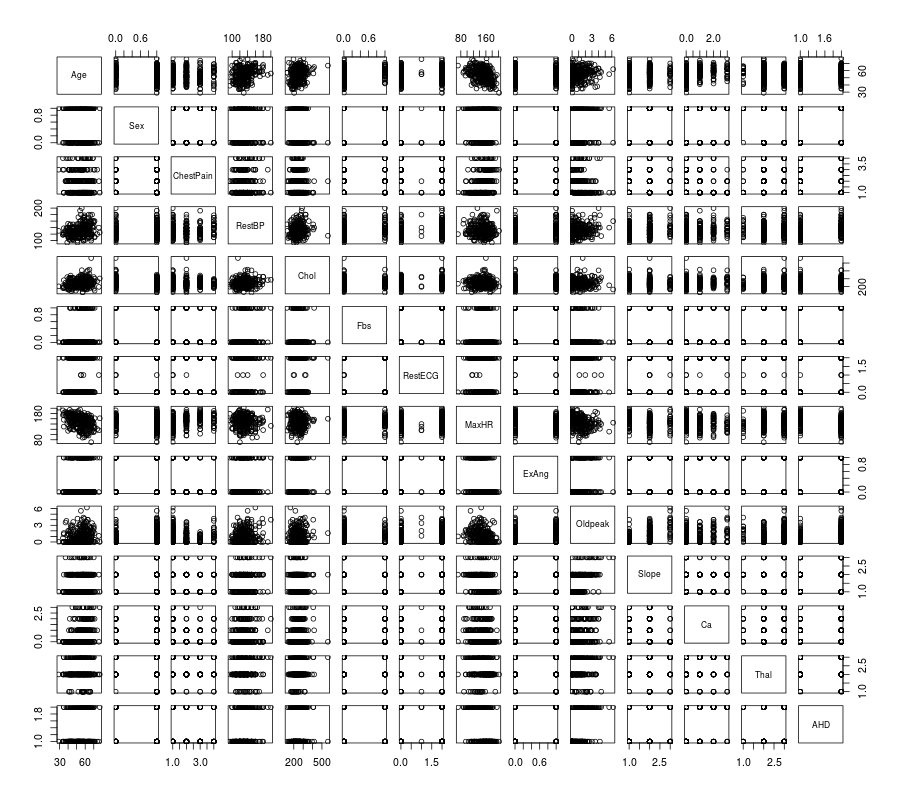
\includegraphics{sumr.png}}
\caption{Summary plot of the data with R.}\label{dap:fig-sumr}\end{figure}
\end{quote}
\begin{itemize}
\item {} 
Summary plot in \textbf{Python}

\end{itemize}
\begin{quote}

\begin{Verbatim}[commandchars=\\\{\}]
\PYG{c}{\PYGZsh{} plot of the summary}
\PYG{n}{plot}\PYG{p}{(}\PYG{n}{rawdata}\PYG{p}{)}
\end{Verbatim}

Then you will get Figure {\hyperref[dap:fig-sump]{\emph{Summary plot of the data with Python.}}}
\begin{figure}[htbp]
\centering
\capstart

\scalebox{0.500000}{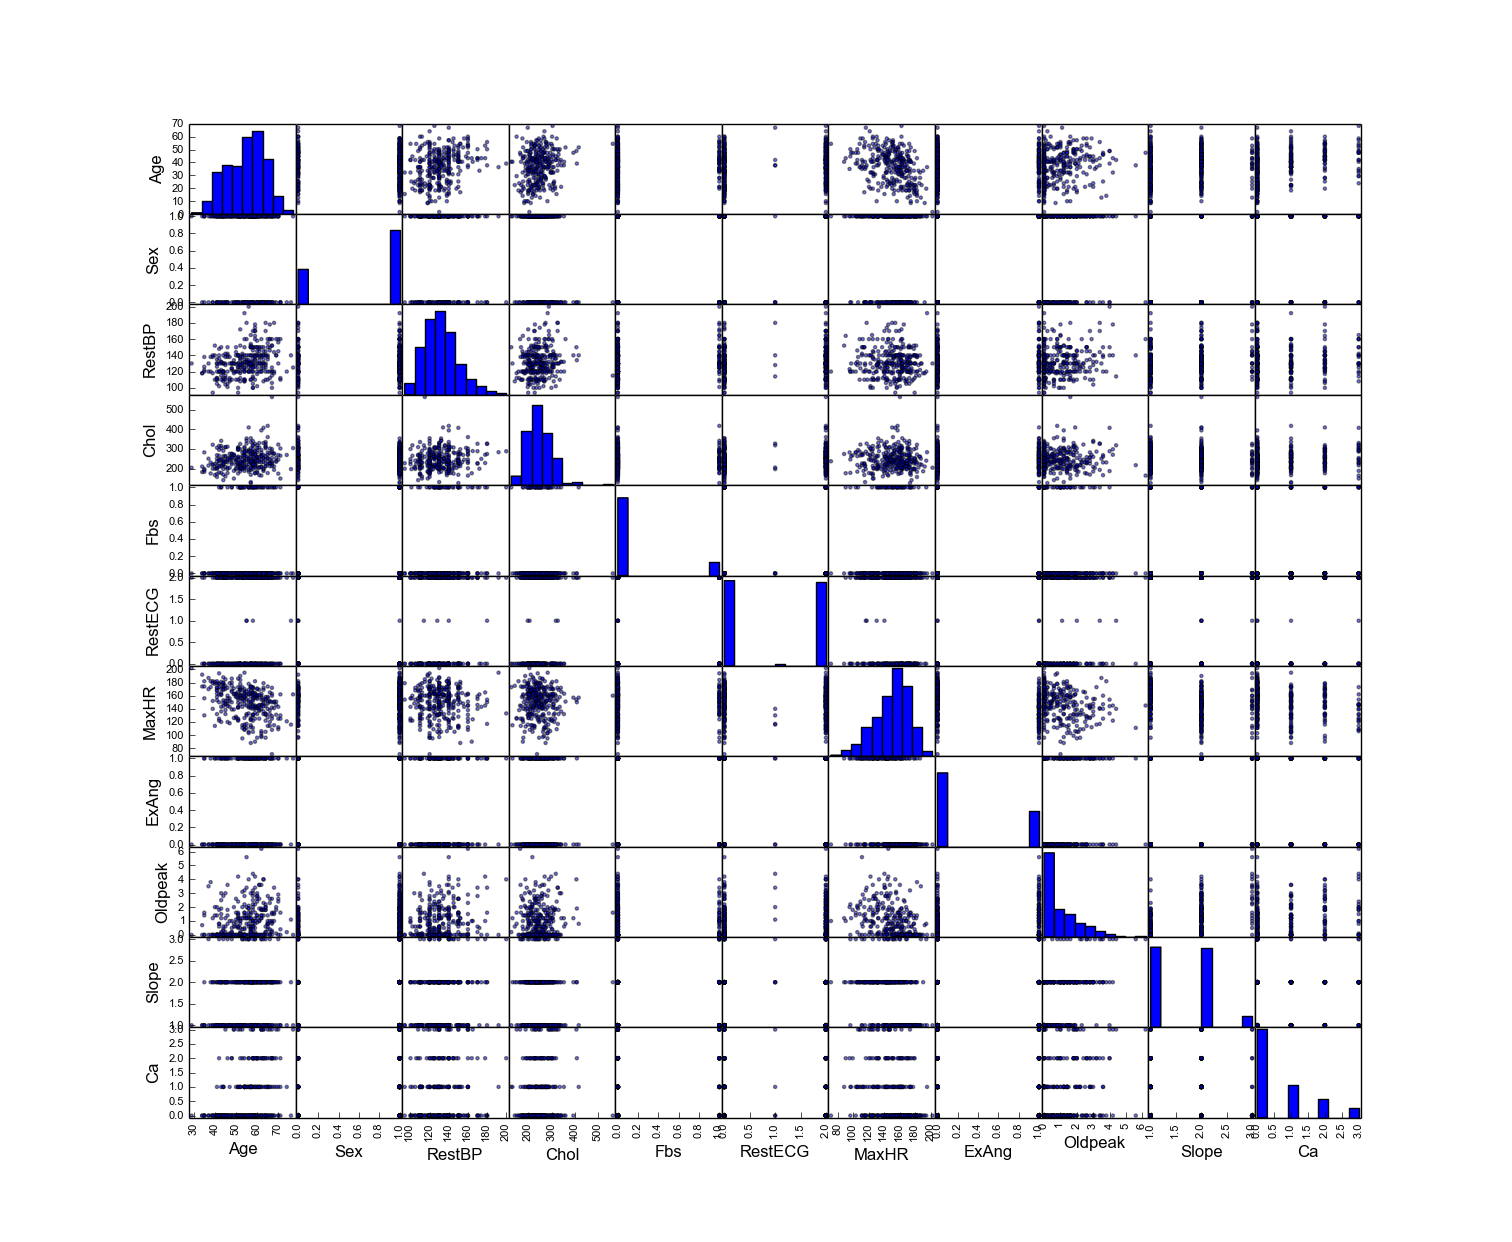
\includegraphics{sumPython.png}}
\caption{Summary plot of the data with Python.}\label{dap:fig-sump}\end{figure}
\end{quote}
\end{quote}
\begin{enumerate}
\setcounter{enumi}{1}
\item {} 
Histogram of the quantitative predictors

\end{enumerate}
\begin{quote}
\begin{itemize}
\item {} 
Histogram in \textbf{R}

\end{itemize}
\begin{quote}

\begin{Verbatim}[commandchars=\\\{\}]
\PYG{c+c1}{\PYGZsh{} Histogram with normal curve plot}
dev.off\PYG{p}{(}\PYG{p}{)}
Nvars\PYG{o}{=}ncol\PYG{p}{(}numdata\PYG{p}{)}
name\PYG{o}{=}colnames\PYG{p}{(}numdata\PYG{p}{)}
par\PYG{p}{(}mfrow \PYG{o}{=}c \PYG{p}{(}\PYG{l+m}{4}\PYG{p}{,}\PYG{l+m}{3}\PYG{p}{)}\PYG{p}{)}
\PYG{k+kr}{for} \PYG{p}{(}i \PYG{k+kr}{in} \PYG{l+m}{1}\PYG{o}{:}Nvars\PYG{p}{)}
\PYG{p}{\PYGZob{}}
  x\PYG{o}{\PYGZlt{}\PYGZhy{}} numdata\PYG{p}{[}\PYG{p}{,}i\PYG{p}{]}
  h\PYG{o}{\PYGZlt{}\PYGZhy{}}hist\PYG{p}{(}x\PYG{p}{,} breaks\PYG{o}{=}\PYG{l+m}{10}\PYG{p}{,} freq\PYG{o}{=}\PYG{k+kc}{TRUE}\PYG{p}{,} col\PYG{o}{=}\PYG{l+s}{\PYGZdq{}}\PYG{l+s}{blue\PYGZdq{}}\PYG{p}{,} xlab\PYG{o}{=}name\PYG{p}{[}i\PYG{p}{]}\PYG{p}{,}main\PYG{o}{=}\PYG{l+s}{\PYGZdq{}}\PYG{l+s}{ \PYGZdq{}}\PYG{p}{,}
            font.lab\PYG{o}{=}\PYG{l+m}{1}\PYG{p}{)}
  axis\PYG{p}{(}\PYG{l+m}{1}\PYG{p}{,} tck\PYG{o}{=}\PYG{l+m}{1}\PYG{p}{,} col.ticks\PYG{o}{=}\PYG{l+s}{\PYGZdq{}}\PYG{l+s}{light gray\PYGZdq{}}\PYG{p}{)}
  axis\PYG{p}{(}\PYG{l+m}{1}\PYG{p}{,} tck\PYG{o}{=}\PYG{l+m}{\PYGZhy{}0.015}\PYG{p}{,} col.ticks\PYG{o}{=}\PYG{l+s}{\PYGZdq{}}\PYG{l+s}{black\PYGZdq{}}\PYG{p}{)}
  axis\PYG{p}{(}\PYG{l+m}{2}\PYG{p}{,} tck\PYG{o}{=}\PYG{l+m}{1}\PYG{p}{,} col.ticks\PYG{o}{=}\PYG{l+s}{\PYGZdq{}}\PYG{l+s}{light gray\PYGZdq{}}\PYG{p}{,} lwd.ticks\PYG{o}{=}\PYG{l+s}{\PYGZdq{}}\PYG{l+s}{1\PYGZdq{}}\PYG{p}{)}
  axis\PYG{p}{(}\PYG{l+m}{2}\PYG{p}{,} tck\PYG{o}{=}\PYG{l+m}{\PYGZhy{}0.015}\PYG{p}{)}
  xfit\PYG{o}{\PYGZlt{}\PYGZhy{}}seq\PYG{p}{(}min\PYG{p}{(}x\PYG{p}{)}\PYG{p}{,}max\PYG{p}{(}x\PYG{p}{)}\PYG{p}{,}length\PYG{o}{=}\PYG{l+m}{40}\PYG{p}{)}
  yfit\PYG{o}{\PYGZlt{}\PYGZhy{}}dnorm\PYG{p}{(}xfit\PYG{p}{,}mean\PYG{o}{=}mean\PYG{p}{(}x\PYG{p}{)}\PYG{p}{,}sd\PYG{o}{=}sd\PYG{p}{(}x\PYG{p}{)}\PYG{p}{)}
  yfit \PYG{o}{\PYGZlt{}\PYGZhy{}} yfit\PYG{o}{*}diff\PYG{p}{(}h\PYG{o}{\PYGZdl{}}mids\PYG{p}{[}\PYG{l+m}{1}\PYG{o}{:}\PYG{l+m}{2}\PYG{p}{]}\PYG{p}{)}\PYG{o}{*}length\PYG{p}{(}x\PYG{p}{)}
  lines\PYG{p}{(}xfit\PYG{p}{,} yfit\PYG{p}{,} col\PYG{o}{=}\PYG{l+s}{\PYGZdq{}}\PYG{l+s}{blue\PYGZdq{}}\PYG{p}{,} lwd\PYG{o}{=}\PYG{l+m}{2}\PYG{p}{)}
\PYG{p}{\PYGZcb{}}
\end{Verbatim}

Then you will get Figure {\hyperref[dap:fig-histr]{\emph{Histogram with normal curve plot in R.}}}
\begin{figure}[htbp]
\centering
\capstart

\scalebox{0.600000}{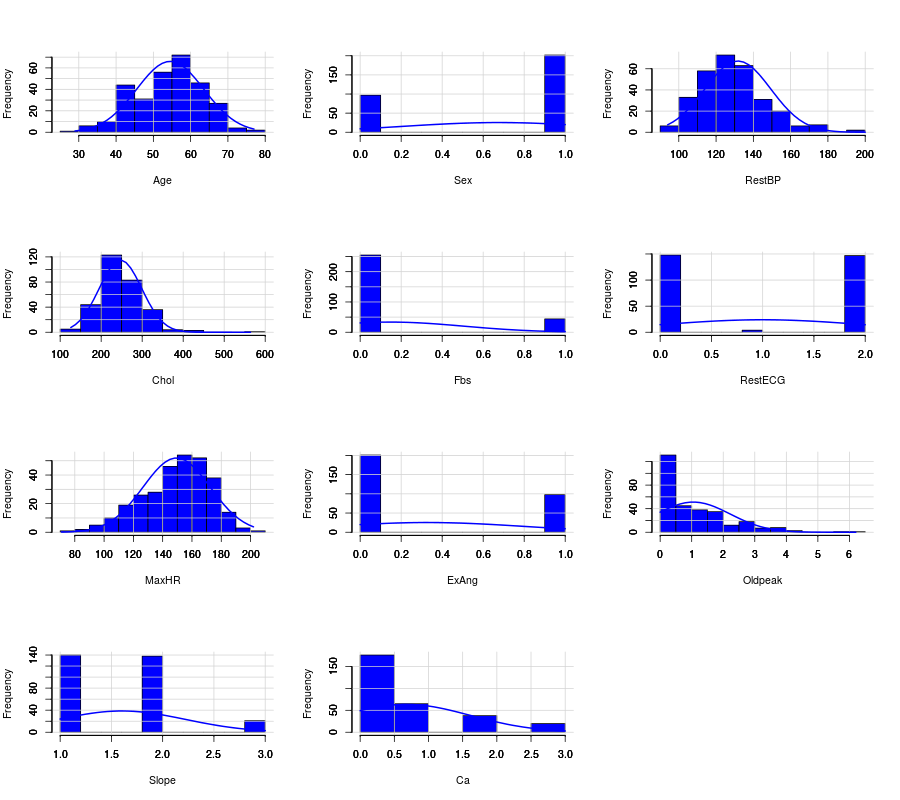
\includegraphics{histr.png}}
\caption{Histogram with normal curve plot in R.}\label{dap:fig-histr}\end{figure}
\end{quote}
\begin{itemize}
\item {} 
Histogram in in \textbf{Python}

\end{itemize}
\begin{quote}

\begin{Verbatim}[commandchars=\\\{\}]
\PYG{c}{\PYGZsh{} Histogram}
\PYG{n}{rawdata}\PYG{o}{.}\PYG{n}{hist}\PYG{p}{(}\PYG{p}{)}
\PYG{n}{plt}\PYG{o}{.}\PYG{n}{show}\PYG{p}{(}\PYG{p}{)}
\end{Verbatim}

Then you will get Figure {\hyperref[dap:fig-histp]{\emph{Histogram in Python.}}}
\begin{figure}[htbp]
\centering
\capstart

\scalebox{0.500000}{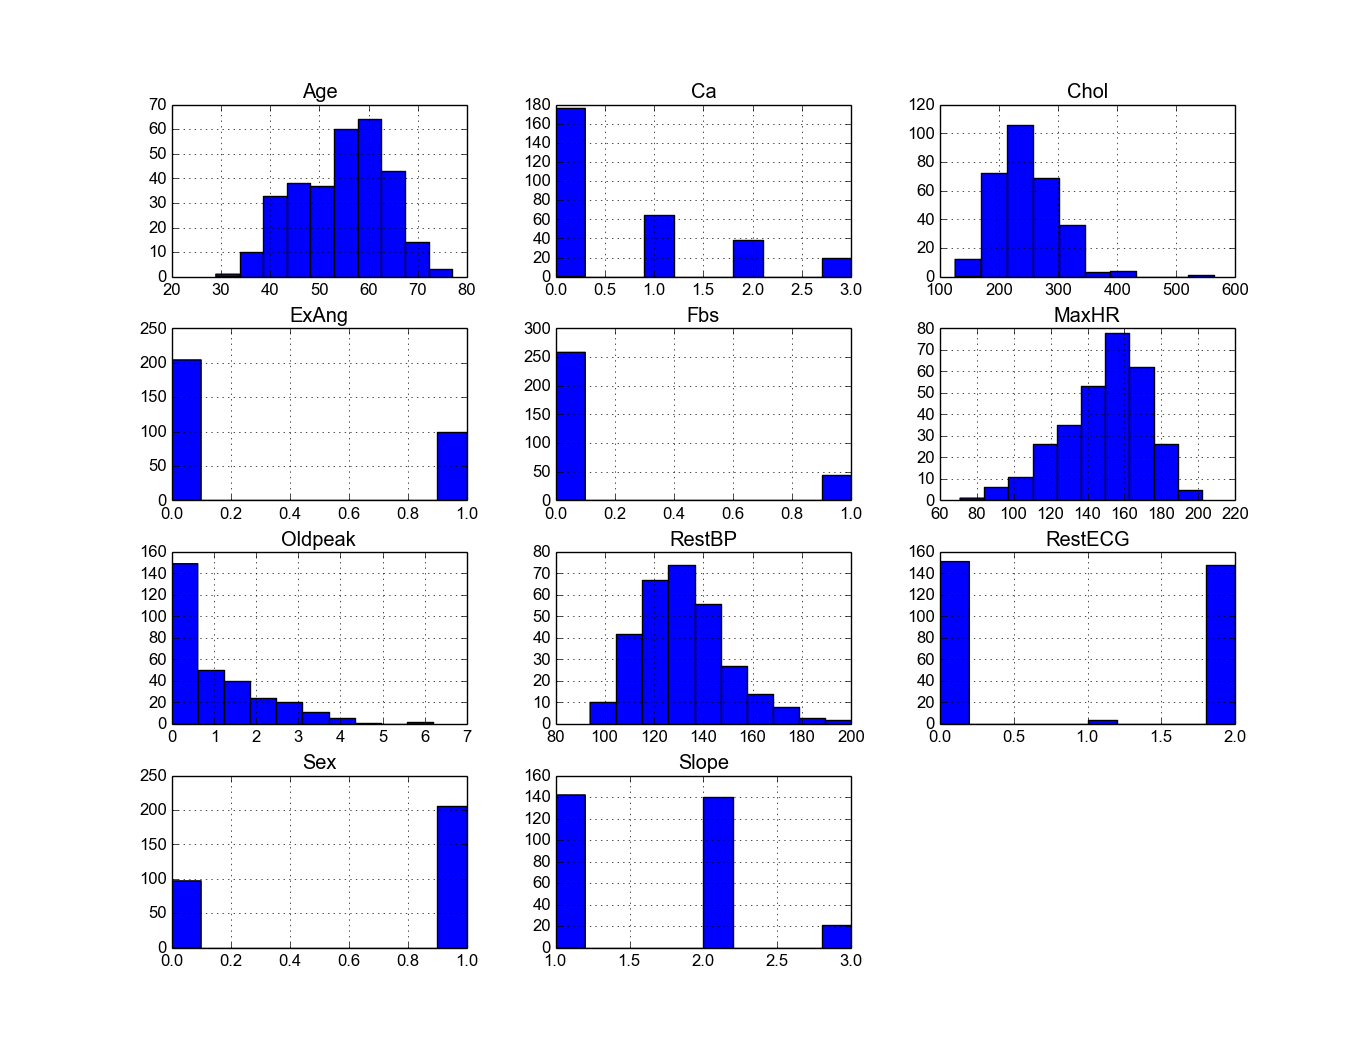
\includegraphics{histp.png}}
\caption{Histogram in Python.}\label{dap:fig-histp}\end{figure}
\end{quote}
\end{quote}
\begin{enumerate}
\setcounter{enumi}{2}
\item {} 
Boxplot of the quantitative predictors

\end{enumerate}
\begin{quote}
\begin{itemize}
\item {} 
Boxplot in \textbf{R}

\end{itemize}
\begin{quote}

\begin{Verbatim}[commandchars=\\\{\}]
dev.off\PYG{p}{(}\PYG{p}{)}
name\PYG{o}{=}colnames\PYG{p}{(}numdata\PYG{p}{)}
    Nvars\PYG{o}{=}ncol\PYG{p}{(}numdata\PYG{p}{)}
    \PYG{c+c1}{\PYGZsh{} boxplot}
    par\PYG{p}{(}mfrow \PYG{o}{=}c \PYG{p}{(}\PYG{l+m}{4}\PYG{p}{,}\PYG{l+m}{3}\PYG{p}{)}\PYG{p}{)}
    \PYG{k+kr}{for} \PYG{p}{(}i \PYG{k+kr}{in} \PYG{l+m}{1}\PYG{o}{:}Nvars\PYG{p}{)}
    \PYG{p}{\PYGZob{}}
     \PYG{c+c1}{\PYGZsh{}boxplot(numdata[,i]\PYGZti{}numdata[,Nvars],data=data,main=name[i])}
     boxplot\PYG{p}{(}numdata\PYG{p}{[}\PYG{p}{,}i\PYG{p}{]}\PYG{p}{,}data\PYG{o}{=}numdata\PYG{p}{,}main\PYG{o}{=}name\PYG{p}{[}i\PYG{p}{]}\PYG{p}{)}
    \PYG{p}{\PYGZcb{}}
\end{Verbatim}

Then you will get Figure {\hyperref[dap:fig-boxr]{\emph{Boxplots in R.}}}
\begin{figure}[htbp]
\centering
\capstart

\scalebox{0.600000}{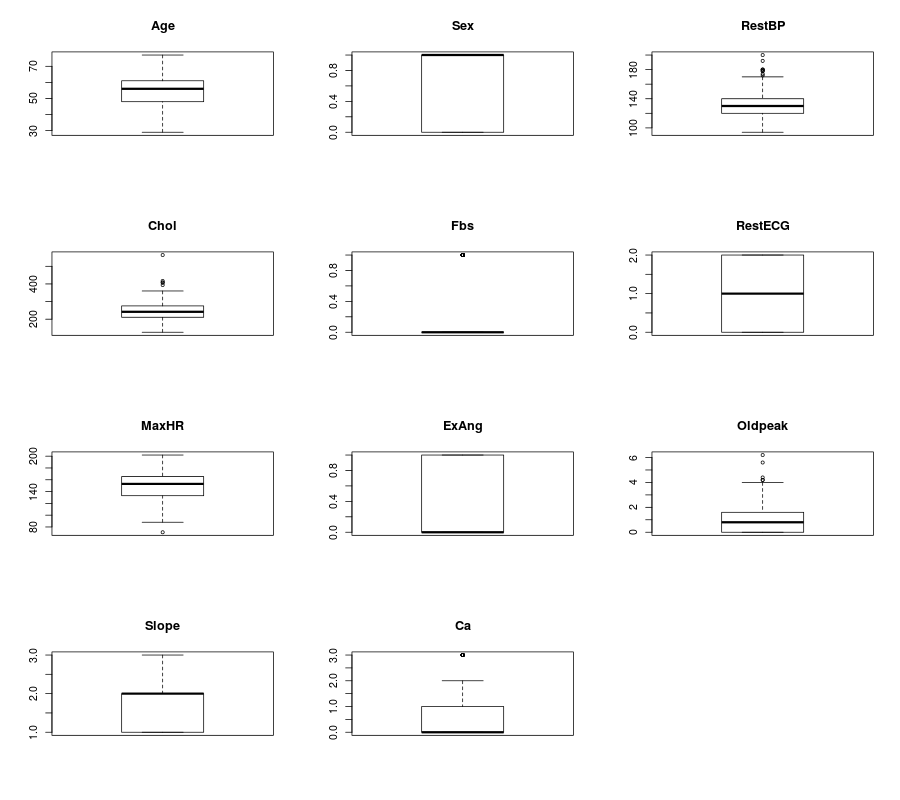
\includegraphics{boxr.png}}
\caption{Boxplots in R.}\label{dap:fig-boxr}\end{figure}
\end{quote}
\begin{itemize}
\item {} 
Boxplot in \textbf{Python}

\end{itemize}
\begin{quote}

\begin{Verbatim}[commandchars=\\\{\}]
\PYG{c}{\PYGZsh{} boxplot}
\PYG{n}{pd}\PYG{o}{.}\PYG{n}{DataFrame}\PYG{o}{.}\PYG{n}{boxplot}\PYG{p}{(}\PYG{n}{rawdata}\PYG{p}{)}
\PYG{n}{plt}\PYG{o}{.}\PYG{n}{show}\PYG{p}{(}\PYG{p}{)}
\end{Verbatim}

Then you will get Figure {\hyperref[dap:fig-boxp]{\emph{Histogram in Python.}}}
\begin{figure}[htbp]
\centering
\capstart

\scalebox{0.600000}{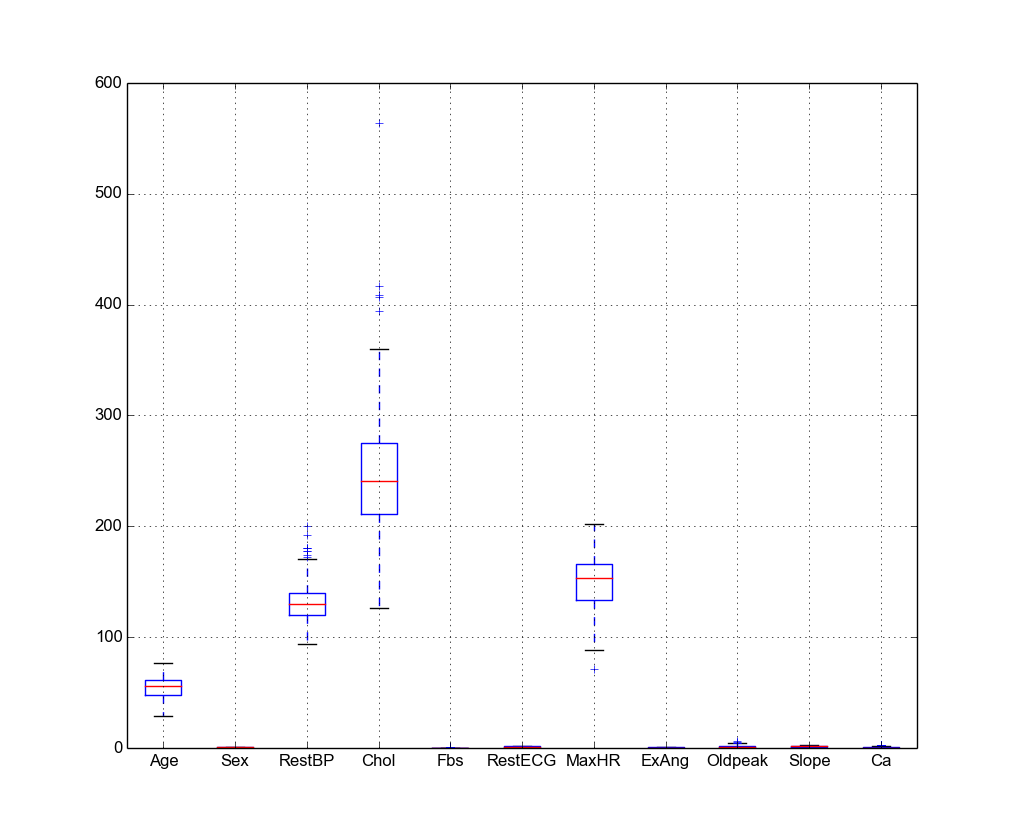
\includegraphics{boxp.png}}
\caption{Histogram in Python.}\label{dap:fig-boxp}\end{figure}
\end{quote}
\end{quote}
\begin{enumerate}
\setcounter{enumi}{3}
\item {} 
Correlation Matrix plot of the quantitative predictors

\end{enumerate}
\begin{quote}
\begin{itemize}
\item {} 
Correlation Matrix plot in \textbf{R}

\end{itemize}
\begin{quote}

\begin{Verbatim}[commandchars=\\\{\}]
dev.off\PYG{p}{(}\PYG{p}{)}
\PYG{c+c1}{\PYGZsh{} laod cocorrelation Matrix plot lib}
library\PYG{p}{(}corrplot\PYG{p}{)}
M \PYG{o}{\PYGZlt{}\PYGZhy{}} cor\PYG{p}{(}numdata\PYG{p}{)}
\PYG{c+c1}{\PYGZsh{}par(mfrow =c (1,2))}
\PYG{c+c1}{\PYGZsh{}corrplot(M, method = \PYGZdq{}square\PYGZdq{})}
corrplot.mixed\PYG{p}{(}M\PYG{p}{)}
\end{Verbatim}

Then you will get Figure {\hyperref[dap:fig-corr]{\emph{Correlation Matrix plot  in R.}}}
\begin{figure}[htbp]
\centering
\capstart

\scalebox{0.600000}{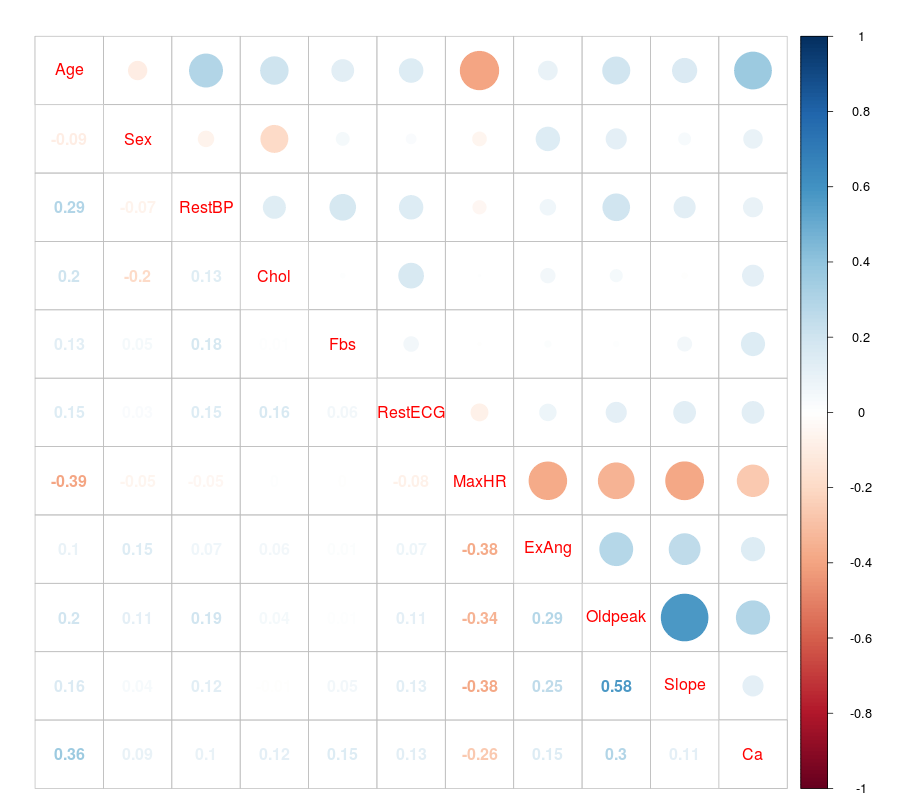
\includegraphics{corr.png}}
\caption{Correlation Matrix plot  in R.}\label{dap:fig-corr}\end{figure}
\end{quote}
\begin{itemize}
\item {} 
Correlation Matrix plot in \textbf{Python}

\end{itemize}
\begin{quote}

\begin{Verbatim}[commandchars=\\\{\}]
\PYG{c}{\PYGZsh{} cocorrelation Matrix plot}
\PYG{n}{pd}\PYG{o}{.}\PYG{n}{DataFrame}\PYG{o}{.}\PYG{n}{corr}\PYG{p}{(}\PYG{n}{rawdata}\PYG{p}{)}
\PYG{n}{plt}\PYG{o}{.}\PYG{n}{show}\PYG{p}{(}\PYG{p}{)}
\end{Verbatim}

Then you will get get Figure {\hyperref[dap:fig-corp]{\emph{Correlation Matrix plot  in Python.}}}
\begin{figure}[htbp]
\centering
\capstart

\scalebox{0.600000}{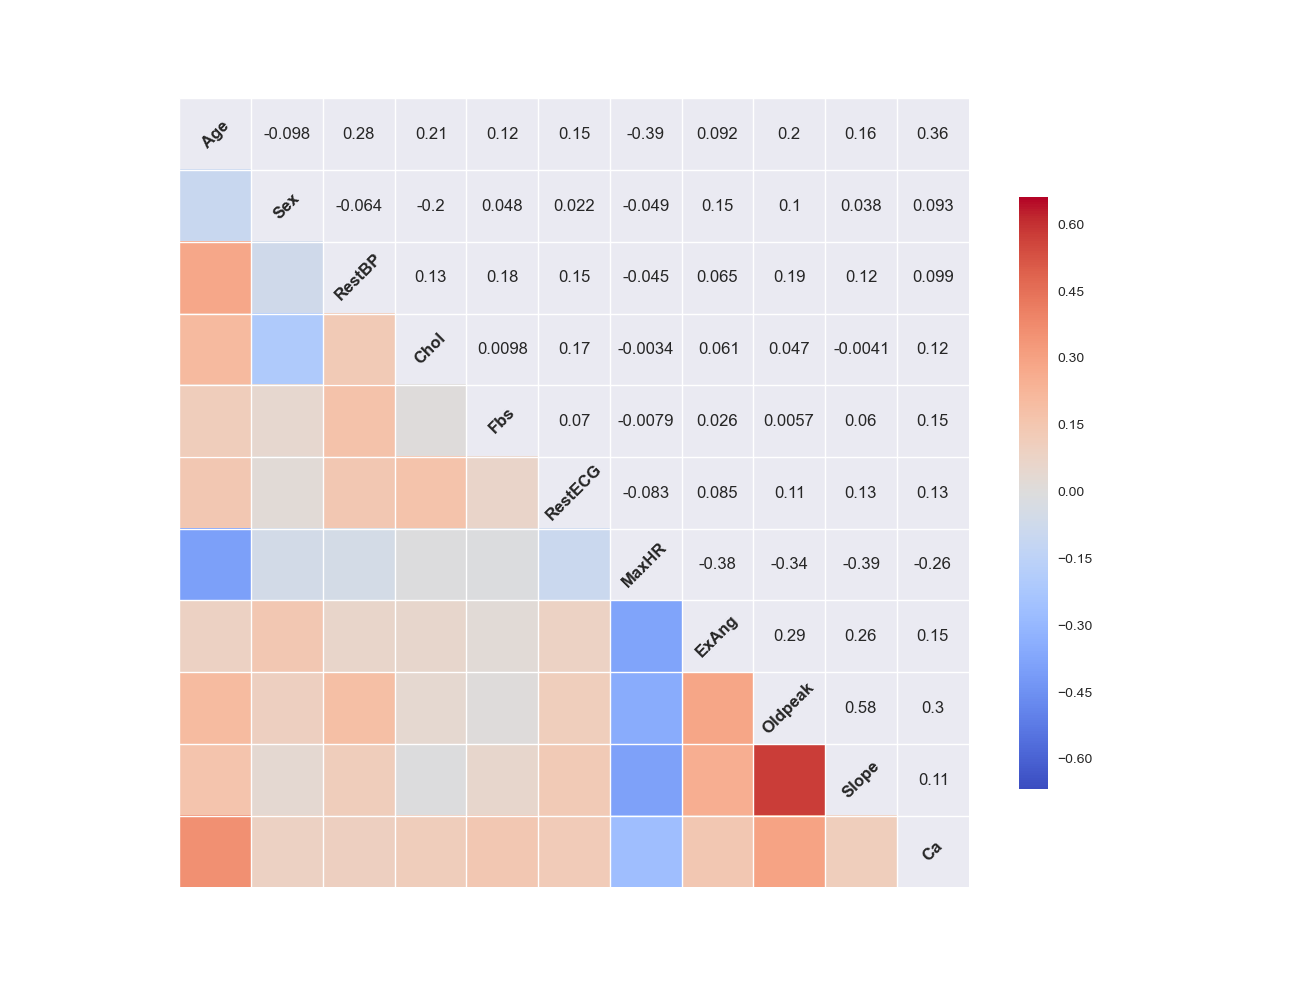
\includegraphics{corp.png}}
\caption{Correlation Matrix plot  in Python.}\label{dap:fig-corp}\end{figure}
\end{quote}
\end{quote}


\section{Source Code for This Section}
\label{dap:source-code-for-this-section}\begin{description}
\item[{The code for this section is available for download for R, for Python,}] \leavevmode\begin{itemize}
\item {} 
R Source code

\end{itemize}
\begin{quote}

\begin{Verbatim}[commandchars=\\\{\}]
rm\PYG{p}{(}list \PYG{o}{=} ls\PYG{p}{(}\PYG{p}{)}\PYG{p}{)}
\PYG{c+c1}{\PYGZsh{} set the enverionment }
path \PYG{o}{=}\PYG{l+s}{\PYGZsq{}}\PYG{l+s}{\PYGZti{}/Dropbox/MachineLearningAlgorithms/python\PYGZus{}code/data/Heart.csv\PYGZsq{}}
rawdata \PYG{o}{=} read.csv\PYG{p}{(}path\PYG{p}{)}

\PYG{c+c1}{\PYGZsh{} summary of the data}
summary\PYG{p}{(}rawdata\PYG{p}{)}
\PYG{c+c1}{\PYGZsh{} plot of the summary}
plot\PYG{p}{(}rawdata\PYG{p}{)}

dim\PYG{p}{(}rawdata\PYG{p}{)}
head\PYG{p}{(}rawdata\PYG{p}{)}
tail\PYG{p}{(}rawdata\PYG{p}{)}

colnames\PYG{p}{(}rawdata\PYG{p}{)}
attach\PYG{p}{(}rawdata\PYG{p}{)}

\PYG{c+c1}{\PYGZsh{} get numerical data and remove NAN}
numdata\PYG{o}{=}na.omit\PYG{p}{(}rawdata\PYG{p}{[}\PYG{p}{,}c\PYG{p}{(}\PYG{l+m}{1}\PYG{o}{:}\PYG{l+m}{2}\PYG{p}{,}\PYG{l+m}{4}\PYG{o}{:}\PYG{l+m}{12}\PYG{p}{)}\PYG{p}{]}\PYG{p}{)}

cor\PYG{p}{(}numdata\PYG{p}{)}
cov\PYG{p}{(}numdata\PYG{p}{)}

dev.off\PYG{p}{(}\PYG{p}{)}
\PYG{c+c1}{\PYGZsh{} laod cocorrelation Matrix plot lib}
library\PYG{p}{(}corrplot\PYG{p}{)}
M \PYG{o}{\PYGZlt{}\PYGZhy{}} cor\PYG{p}{(}numdata\PYG{p}{)}
\PYG{c+c1}{\PYGZsh{}par(mfrow =c (1,2))}
\PYG{c+c1}{\PYGZsh{}corrplot(M, method = \PYGZdq{}square\PYGZdq{})}
corrplot.mixed\PYG{p}{(}M\PYG{p}{)}


nrow\PYG{o}{=}nrow\PYG{p}{(}rawdata\PYG{p}{)}
ncol\PYG{o}{=}ncol\PYG{p}{(}rawdata\PYG{p}{)}
c\PYG{p}{(}nrow\PYG{p}{,} ncol\PYG{p}{)}



Nvars\PYG{o}{=}ncol\PYG{p}{(}numdata\PYG{p}{)}
\PYG{c+c1}{\PYGZsh{} checking data format }
typeof\PYG{p}{(}rawdata\PYG{p}{)}
install.packages\PYG{p}{(}\PYG{l+s}{\PYGZdq{}}\PYG{l+s}{mlbench\PYGZdq{}}\PYG{p}{)}
library\PYG{p}{(}mlbench\PYG{p}{)}
sapply\PYG{p}{(}rawdata\PYG{p}{,} class\PYG{p}{)}

dev.off\PYG{p}{(}\PYG{p}{)}
name\PYG{o}{=}colnames\PYG{p}{(}numdata\PYG{p}{)}
Nvars\PYG{o}{=}ncol\PYG{p}{(}numdata\PYG{p}{)}
\PYG{c+c1}{\PYGZsh{} boxplot }
par\PYG{p}{(}mfrow \PYG{o}{=}c \PYG{p}{(}\PYG{l+m}{4}\PYG{p}{,}\PYG{l+m}{3}\PYG{p}{)}\PYG{p}{)}
\PYG{k+kr}{for} \PYG{p}{(}i \PYG{k+kr}{in} \PYG{l+m}{1}\PYG{o}{:}Nvars\PYG{p}{)}
\PYG{p}{\PYGZob{}}
  \PYG{c+c1}{\PYGZsh{}boxplot(numdata[,i]\PYGZti{}numdata[,Nvars],data=data,main=name[i])}
  boxplot\PYG{p}{(}numdata\PYG{p}{[}\PYG{p}{,}i\PYG{p}{]}\PYG{p}{,}data\PYG{o}{=}numdata\PYG{p}{,}main\PYG{o}{=}name\PYG{p}{[}i\PYG{p}{]}\PYG{p}{)}
\PYG{p}{\PYGZcb{}}

\PYG{c+c1}{\PYGZsh{} Histogram with normal curve plot }
dev.off\PYG{p}{(}\PYG{p}{)}
Nvars\PYG{o}{=}ncol\PYG{p}{(}numdata\PYG{p}{)}
name\PYG{o}{=}colnames\PYG{p}{(}numdata\PYG{p}{)}
par\PYG{p}{(}mfrow \PYG{o}{=}c \PYG{p}{(}\PYG{l+m}{3}\PYG{p}{,}\PYG{l+m}{5}\PYG{p}{)}\PYG{p}{)}
\PYG{k+kr}{for} \PYG{p}{(}i \PYG{k+kr}{in} \PYG{l+m}{1}\PYG{o}{:}Nvars\PYG{p}{)}
\PYG{p}{\PYGZob{}}
  x\PYG{o}{\PYGZlt{}\PYGZhy{}} numdata\PYG{p}{[}\PYG{p}{,}i\PYG{p}{]}
  h\PYG{o}{\PYGZlt{}\PYGZhy{}}hist\PYG{p}{(}x\PYG{p}{,} breaks\PYG{o}{=}\PYG{l+m}{10}\PYG{p}{,} freq\PYG{o}{=}\PYG{k+kc}{TRUE}\PYG{p}{,} col\PYG{o}{=}\PYG{l+s}{\PYGZdq{}}\PYG{l+s}{blue\PYGZdq{}}\PYG{p}{,} xlab\PYG{o}{=}name\PYG{p}{[}i\PYG{p}{]}\PYG{p}{,}main\PYG{o}{=}\PYG{l+s}{\PYGZdq{}}\PYG{l+s}{ \PYGZdq{}}\PYG{p}{,} 
            font.lab\PYG{o}{=}\PYG{l+m}{1}\PYG{p}{)} 
  axis\PYG{p}{(}\PYG{l+m}{1}\PYG{p}{,} tck\PYG{o}{=}\PYG{l+m}{1}\PYG{p}{,} col.ticks\PYG{o}{=}\PYG{l+s}{\PYGZdq{}}\PYG{l+s}{light gray\PYGZdq{}}\PYG{p}{)}
  axis\PYG{p}{(}\PYG{l+m}{1}\PYG{p}{,} tck\PYG{o}{=}\PYG{l+m}{\PYGZhy{}0.015}\PYG{p}{,} col.ticks\PYG{o}{=}\PYG{l+s}{\PYGZdq{}}\PYG{l+s}{black\PYGZdq{}}\PYG{p}{)}
  axis\PYG{p}{(}\PYG{l+m}{2}\PYG{p}{,} tck\PYG{o}{=}\PYG{l+m}{1}\PYG{p}{,} col.ticks\PYG{o}{=}\PYG{l+s}{\PYGZdq{}}\PYG{l+s}{light gray\PYGZdq{}}\PYG{p}{,} lwd.ticks\PYG{o}{=}\PYG{l+s}{\PYGZdq{}}\PYG{l+s}{1\PYGZdq{}}\PYG{p}{)}
  axis\PYG{p}{(}\PYG{l+m}{2}\PYG{p}{,} tck\PYG{o}{=}\PYG{l+m}{\PYGZhy{}0.015}\PYG{p}{)}
  xfit\PYG{o}{\PYGZlt{}\PYGZhy{}}seq\PYG{p}{(}min\PYG{p}{(}x\PYG{p}{)}\PYG{p}{,}max\PYG{p}{(}x\PYG{p}{)}\PYG{p}{,}length\PYG{o}{=}\PYG{l+m}{40}\PYG{p}{)} 
  yfit\PYG{o}{\PYGZlt{}\PYGZhy{}}dnorm\PYG{p}{(}xfit\PYG{p}{,}mean\PYG{o}{=}mean\PYG{p}{(}x\PYG{p}{)}\PYG{p}{,}sd\PYG{o}{=}sd\PYG{p}{(}x\PYG{p}{)}\PYG{p}{)} 
  yfit \PYG{o}{\PYGZlt{}\PYGZhy{}} yfit\PYG{o}{*}diff\PYG{p}{(}h\PYG{o}{\PYGZdl{}}mids\PYG{p}{[}\PYG{l+m}{1}\PYG{o}{:}\PYG{l+m}{2}\PYG{p}{]}\PYG{p}{)}\PYG{o}{*}length\PYG{p}{(}x\PYG{p}{)} 
  lines\PYG{p}{(}xfit\PYG{p}{,} yfit\PYG{p}{,} col\PYG{o}{=}\PYG{l+s}{\PYGZdq{}}\PYG{l+s}{blue\PYGZdq{}}\PYG{p}{,} lwd\PYG{o}{=}\PYG{l+m}{2}\PYG{p}{)} 
\PYG{p}{\PYGZcb{}} 


library\PYG{p}{(}reshape2\PYG{p}{)}
library\PYG{p}{(}ggplot2\PYG{p}{)}
d \PYG{o}{\PYGZlt{}\PYGZhy{}} melt\PYG{p}{(}diamonds\PYG{p}{[}\PYG{p}{,}\PYG{o}{\PYGZhy{}}c\PYG{p}{(}\PYG{l+m}{2}\PYG{o}{:}\PYG{l+m}{4}\PYG{p}{)}\PYG{p}{]}\PYG{p}{)}
ggplot\PYG{p}{(}d\PYG{p}{,}aes\PYG{p}{(}x \PYG{o}{=} value\PYG{p}{)}\PYG{p}{)} \PYG{o}{+} 
  facet\PYGZus{}wrap\PYG{p}{(}\PYG{o}{\PYGZti{}}variable\PYG{p}{,}scales \PYG{o}{=} \PYG{l+s}{\PYGZdq{}}\PYG{l+s}{free\PYGZus{}x\PYGZdq{}}\PYG{p}{)} \PYG{o}{+} 
  geom\PYGZus{}histogram\PYG{p}{(}\PYG{p}{)}
\end{Verbatim}
\end{quote}
\begin{itemize}
\item {} 
Python Source code

\end{itemize}
\begin{quote}

\begin{Verbatim}[commandchars=\\\{\}]
\PYG{l+s+sd}{\PYGZsq{}\PYGZsq{}\PYGZsq{}}
\PYG{l+s+sd}{Created on Apr 25, 2016}
\PYG{l+s+sd}{test code }
\PYG{l+s+sd}{@author: Wenqiang Feng }
\PYG{l+s+sd}{\PYGZsq{}\PYGZsq{}\PYGZsq{}}
\PYG{k+kn}{import} \PYG{n+nn}{pandas} \PYG{k+kn}{as} \PYG{n+nn}{pd}
\PYG{c}{\PYGZsh{}import numpy as np}
\PYG{k+kn}{import} \PYG{n+nn}{matplotlib.pyplot} \PYG{k+kn}{as} \PYG{n+nn}{plt}
\PYG{k+kn}{from} \PYG{n+nn}{pandas.tools.plotting} \PYG{k+kn}{import} \PYG{n}{scatter\PYGZus{}matrix}
\PYG{k+kn}{from} \PYG{n+nn}{docutils.parsers.rst.directives} \PYG{k+kn}{import} \PYG{n}{path}

\PYG{k}{if} \PYG{n}{\PYGZus{}\PYGZus{}name\PYGZus{}\PYGZus{}} \PYG{o}{==} \PYG{l+s}{\PYGZsq{}}\PYG{l+s}{\PYGZus{}\PYGZus{}main\PYGZus{}\PYGZus{}}\PYG{l+s}{\PYGZsq{}}\PYG{p}{:}
    \PYG{n}{path} \PYG{o}{=}\PYG{l+s}{\PYGZsq{}}\PYG{l+s}{\PYGZti{}/Dropbox/MachineLearningAlgorithms/python\PYGZus{}code/data/Heart.csv}\PYG{l+s}{\PYGZsq{}} 
    \PYG{n}{rawdata} \PYG{o}{=} \PYG{n}{pd}\PYG{o}{.}\PYG{n}{read\PYGZus{}csv}\PYG{p}{(}\PYG{n}{path}\PYG{p}{)}
    
    \PYG{k}{print} \PYG{l+s}{\PYGZdq{}}\PYG{l+s}{data summary}\PYG{l+s}{\PYGZdq{}}
    \PYG{k}{print} \PYG{n}{rawdata}\PYG{o}{.}\PYG{n}{describe}\PYG{p}{(}\PYG{p}{)}
    
    \PYG{c}{\PYGZsh{} summary plot of the data}
    \PYG{n}{scatter\PYGZus{}matrix}\PYG{p}{(}\PYG{n}{rawdata}\PYG{p}{,}\PYG{n}{figsize}\PYG{o}{=}\PYG{p}{[}\PYG{l+m+mi}{15}\PYG{p}{,}\PYG{l+m+mi}{15}\PYG{p}{]}\PYG{p}{)}
    \PYG{n}{plt}\PYG{o}{.}\PYG{n}{show}\PYG{p}{(}\PYG{p}{)}
    
    \PYG{c}{\PYGZsh{} Histogram }
    \PYG{n}{rawdata}\PYG{o}{.}\PYG{n}{hist}\PYG{p}{(}\PYG{p}{)}
    \PYG{n}{plt}\PYG{o}{.}\PYG{n}{show}\PYG{p}{(}\PYG{p}{)}
    
    \PYG{c}{\PYGZsh{} boxplot }
    \PYG{n}{pd}\PYG{o}{.}\PYG{n}{DataFrame}\PYG{o}{.}\PYG{n}{boxplot}\PYG{p}{(}\PYG{n}{rawdata}\PYG{p}{)}
    \PYG{n}{plt}\PYG{o}{.}\PYG{n}{show}\PYG{p}{(}\PYG{p}{)}
    
    
    \PYG{k}{print} \PYG{l+s}{\PYGZdq{}}\PYG{l+s}{Raw data size}\PYG{l+s}{\PYGZdq{}}
    \PYG{n}{nrow}\PYG{p}{,} \PYG{n}{ncol} \PYG{o}{=} \PYG{n}{rawdata}\PYG{o}{.}\PYG{n}{shape}
    \PYG{k}{print} \PYG{n}{nrow}\PYG{p}{,} \PYG{n}{ncol}
    
    \PYG{n}{path} \PYG{o}{=} \PYG{p}{(}\PYG{l+s}{\PYGZsq{}}\PYG{l+s}{/home/feng/Dropbox/MachineLearningAlgorithms/python\PYGZus{}code/data/}\PYG{l+s}{\PYGZsq{}}
    \PYG{l+s}{\PYGZsq{}}\PYG{l+s}{energy\PYGZus{}efficiency.xlsx}\PYG{l+s}{\PYGZsq{}}\PYG{p}{)}
    \PYG{n}{path}
            
    \PYG{n}{rawdataEnergy}\PYG{o}{=} \PYG{n}{pd}\PYG{o}{.}\PYG{n}{read\PYGZus{}excel}\PYG{p}{(}\PYG{n}{path}\PYG{p}{,}\PYG{n}{sheetname}\PYG{o}{=}\PYG{l+m+mi}{0}\PYG{p}{)}
    
    \PYG{n}{nrow}\PYG{o}{=}\PYG{n}{rawdata}\PYG{o}{.}\PYG{n}{shape}\PYG{p}{[}\PYG{l+m+mi}{0}\PYG{p}{]} \PYG{c}{\PYGZsh{}gives number of row count}
    \PYG{n}{ncol}\PYG{o}{=}\PYG{n}{rawdata}\PYG{o}{.}\PYG{n}{shape}\PYG{p}{[}\PYG{l+m+mi}{1}\PYG{p}{]} \PYG{c}{\PYGZsh{}gives number of col count}
    \PYG{k}{print} \PYG{n}{nrow}\PYG{p}{,} \PYG{n}{ncol}
    \PYG{n}{col\PYGZus{}names} \PYG{o}{=} \PYG{n}{rawdata}\PYG{o}{.}\PYG{n}{columns}\PYG{o}{.}\PYG{n}{tolist}\PYG{p}{(}\PYG{p}{)}
    \PYG{k}{print} \PYG{l+s}{\PYGZdq{}}\PYG{l+s}{Column names:}\PYG{l+s}{\PYGZdq{}}
    \PYG{k}{print} \PYG{n}{col\PYGZus{}names}
    \PYG{k}{print} \PYG{l+s}{\PYGZdq{}}\PYG{l+s}{Data Format:}\PYG{l+s}{\PYGZdq{}}
    \PYG{k}{print} \PYG{n}{rawdata}\PYG{o}{.}\PYG{n}{dtypes}
    
    \PYG{k}{print} \PYG{l+s}{\PYGZdq{}}\PYG{l+s+se}{\PYGZbs{}n}\PYG{l+s}{Sample data:}\PYG{l+s}{\PYGZdq{}}
    \PYG{k}{print}\PYG{p}{(}\PYG{n}{rawdata}\PYG{o}{.}\PYG{n}{head}\PYG{p}{(}\PYG{l+m+mi}{6}\PYG{p}{)}\PYG{p}{)}
    
    
    \PYG{k}{print} \PYG{l+s}{\PYGZdq{}}\PYG{l+s+se}{\PYGZbs{}n}\PYG{l+s}{ correlation Matrix}\PYG{l+s}{\PYGZdq{}}
    \PYG{k}{print} \PYG{n}{rawdata}\PYG{o}{.}\PYG{n}{corr}\PYG{p}{(}\PYG{p}{)}
    
    \PYG{c}{\PYGZsh{} cocorrelation Matrix plot     }
    \PYG{n}{pd}\PYG{o}{.}\PYG{n}{DataFrame}\PYG{o}{.}\PYG{n}{corr}\PYG{p}{(}\PYG{n}{rawdata}\PYG{p}{)}
    \PYG{n}{plt}\PYG{o}{.}\PYG{n}{show}\PYG{p}{(}\PYG{p}{)}
    
    \PYG{k}{print} \PYG{l+s}{\PYGZdq{}}\PYG{l+s+se}{\PYGZbs{}n}\PYG{l+s}{ covariance Matrix}\PYG{l+s}{\PYGZdq{}}
    \PYG{k}{print} \PYG{n}{rawdata}\PYG{o}{.}\PYG{n}{cov}\PYG{p}{(}\PYG{p}{)}
    
    \PYG{k}{print} \PYG{n}{rawdata}\PYG{p}{[}\PYG{p}{[}\PYG{l+s}{\PYGZsq{}}\PYG{l+s}{Age}\PYG{l+s}{\PYGZsq{}}\PYG{p}{,}\PYG{l+s}{\PYGZsq{}}\PYG{l+s}{Ca}\PYG{l+s}{\PYGZsq{}}\PYG{p}{]}\PYG{p}{]}\PYG{o}{.}\PYG{n}{corr}\PYG{p}{(}\PYG{p}{)}
    \PYG{n}{pd}\PYG{o}{.}\PYG{n}{DataFrame}\PYG{o}{.}\PYG{n}{corr}\PYG{p}{(}\PYG{n}{rawdata}\PYG{p}{)}
    \PYG{n}{plt}\PYG{o}{.}\PYG{n}{show}\PYG{p}{(}\PYG{p}{)}
    

    
    \PYG{c}{\PYGZsh{} define colors list, to be used to plot survived either red (=0) or green (=1)}
    \PYG{n}{colors}\PYG{o}{=}\PYG{p}{[}\PYG{l+s}{\PYGZsq{}}\PYG{l+s}{red}\PYG{l+s}{\PYGZsq{}}\PYG{p}{,}\PYG{l+s}{\PYGZsq{}}\PYG{l+s}{green}\PYG{l+s}{\PYGZsq{}}\PYG{p}{]}

    \PYG{c}{\PYGZsh{} make a scatter plot}

\PYG{c}{\PYGZsh{}    rawdata.info()}

    \PYG{k+kn}{from} \PYG{n+nn}{scipy} \PYG{k+kn}{import} \PYG{n}{stats}
    \PYG{k+kn}{import} \PYG{n+nn}{seaborn} \PYG{k+kn}{as} \PYG{n+nn}{sns} \PYG{c}{\PYGZsh{} just a conventional alias, don\PYGZsq{}t know why}
    \PYG{n}{sns}\PYG{o}{.}\PYG{n}{corrplot}\PYG{p}{(}\PYG{n}{rawdata}\PYG{p}{)} \PYG{c}{\PYGZsh{} compute and plot the pair\PYGZhy{}wise correlations}
    \PYG{c}{\PYGZsh{} save to file, remove the big white borders}
    \PYG{c}{\PYGZsh{}plt.savefig(\PYGZsq{}attribute\PYGZus{}correlations.png\PYGZsq{}, tight\PYGZus{}layout=True)}
    \PYG{n}{plt}\PYG{o}{.}\PYG{n}{show}\PYG{p}{(}\PYG{p}{)}
    
    
    \PYG{n}{attr} \PYG{o}{=} \PYG{n}{rawdata}\PYG{p}{[}\PYG{l+s}{\PYGZsq{}}\PYG{l+s}{Age}\PYG{l+s}{\PYGZsq{}}\PYG{p}{]}
    \PYG{n}{sns}\PYG{o}{.}\PYG{n}{distplot}\PYG{p}{(}\PYG{n}{attr}\PYG{p}{)}
    \PYG{n}{plt}\PYG{o}{.}\PYG{n}{show}\PYG{p}{(}\PYG{p}{)}
    
    \PYG{n}{sns}\PYG{o}{.}\PYG{n}{distplot}\PYG{p}{(}\PYG{n}{attr}\PYG{p}{,} \PYG{n}{kde}\PYG{o}{=}\PYG{n+nb+bp}{False}\PYG{p}{,} \PYG{n}{fit}\PYG{o}{=}\PYG{n}{stats}\PYG{o}{.}\PYG{n}{gamma}\PYG{p}{)}\PYG{p}{;}
    \PYG{n}{plt}\PYG{o}{.}\PYG{n}{show}\PYG{p}{(}\PYG{p}{)}
    
    \PYG{c}{\PYGZsh{} Two subplots, the axes array is 1\PYGZhy{}d}
    \PYG{n}{plt}\PYG{o}{.}\PYG{n}{figure}\PYG{p}{(}\PYG{l+m+mi}{1}\PYG{p}{)}
    \PYG{n}{plt}\PYG{o}{.}\PYG{n}{title}\PYG{p}{(}\PYG{l+s}{\PYGZsq{}}\PYG{l+s}{Histogram of Age}\PYG{l+s}{\PYGZsq{}}\PYG{p}{)}
    \PYG{n}{plt}\PYG{o}{.}\PYG{n}{subplot}\PYG{p}{(}\PYG{l+m+mi}{211}\PYG{p}{)} \PYG{c}{\PYGZsh{} 21,1 means first one of 2 rows, 1 col }
    \PYG{n}{sns}\PYG{o}{.}\PYG{n}{distplot}\PYG{p}{(}\PYG{n}{attr}\PYG{p}{)}
    
    \PYG{n}{plt}\PYG{o}{.}\PYG{n}{subplot}\PYG{p}{(}\PYG{l+m+mi}{212}\PYG{p}{)} \PYG{c}{\PYGZsh{}  21,2 means second one of 2 rows, 1 col }
    \PYG{n}{sns}\PYG{o}{.}\PYG{n}{distplot}\PYG{p}{(}\PYG{n}{attr}\PYG{p}{,} \PYG{n}{kde}\PYG{o}{=}\PYG{n+nb+bp}{False}\PYG{p}{,} \PYG{n}{fit}\PYG{o}{=}\PYG{n}{stats}\PYG{o}{.}\PYG{n}{gamma}\PYG{p}{)}\PYG{p}{;}

    \PYG{n}{plt}\PYG{o}{.}\PYG{n}{show}\PYG{p}{(}\PYG{p}{)}
\end{Verbatim}
\end{quote}

\end{description}
\phantomsection\label{pre:pre}
\index{Pre-processing procedures}

\chapter{Pre-processing procedures}
\label{pre:index-0}\label{pre::doc}\label{pre:pre-processing-procedures}
\begin{notice}{note}{Note:}
\textbf{Well begun is half done} -- old Chinese proverb
\end{notice}

In my opinion,  preprocessing is crucial for the data mining algorithms. If you get a good pre-processing, you will definitely get a beeter result. In this section, we will learn how to do a proper pre-processing in  \textbf{R} and \textbf{Python}.

\index{rough preprocessing}

\section{Rough Pre-processing}
\label{pre:rough-pre-processing}\label{pre:index-1}\begin{itemize}
\item {} 
\textbf{dealing with missing data}

\end{itemize}
\begin{quote}

Usually, we have two popular way to deal with the missing data: replacing by 0 or replacing by mean value.
\begin{itemize}
\item {} 
dealing with missing data in \textbf{R}

\item {} 
dealing with missing data in \textbf{Python}

\end{itemize}
\end{quote}


\section{Source Code for This Section}
\label{pre:source-code-for-this-section}\begin{description}
\item[{The code for this section is available for download for R, for Python,}] \leavevmode\begin{itemize}
\item {} 
R Source code

\end{itemize}
\begin{quote}

\begin{Verbatim}[commandchars=\\\{\}]
rm\PYG{p}{(}list \PYG{o}{=} ls\PYG{p}{(}\PYG{p}{)}\PYG{p}{)}
\PYG{c+c1}{\PYGZsh{} set the enverionment }
path \PYG{o}{=}\PYG{l+s}{\PYGZsq{}}\PYG{l+s}{\PYGZti{}/Dropbox/MachineLearningAlgorithms/python\PYGZus{}code/data/Heart.csv\PYGZsq{}}
rawdata \PYG{o}{=} read.csv\PYG{p}{(}path\PYG{p}{)}

\PYG{c+c1}{\PYGZsh{} summary of the data}
summary\PYG{p}{(}rawdata\PYG{p}{)}
\PYG{c+c1}{\PYGZsh{} plot of the summary}
plot\PYG{p}{(}rawdata\PYG{p}{)}

dim\PYG{p}{(}rawdata\PYG{p}{)}
head\PYG{p}{(}rawdata\PYG{p}{)}
tail\PYG{p}{(}rawdata\PYG{p}{)}

colnames\PYG{p}{(}rawdata\PYG{p}{)}
attach\PYG{p}{(}rawdata\PYG{p}{)}

\PYG{c+c1}{\PYGZsh{} get numerical data and remove NAN}
numdata\PYG{o}{=}na.omit\PYG{p}{(}rawdata\PYG{p}{[}\PYG{p}{,}c\PYG{p}{(}\PYG{l+m}{1}\PYG{o}{:}\PYG{l+m}{2}\PYG{p}{,}\PYG{l+m}{4}\PYG{o}{:}\PYG{l+m}{12}\PYG{p}{)}\PYG{p}{]}\PYG{p}{)}

cor\PYG{p}{(}numdata\PYG{p}{)}
cov\PYG{p}{(}numdata\PYG{p}{)}

dev.off\PYG{p}{(}\PYG{p}{)}
\PYG{c+c1}{\PYGZsh{} laod cocorrelation Matrix plot lib}
library\PYG{p}{(}corrplot\PYG{p}{)}
M \PYG{o}{\PYGZlt{}\PYGZhy{}} cor\PYG{p}{(}numdata\PYG{p}{)}
\PYG{c+c1}{\PYGZsh{}par(mfrow =c (1,2))}
\PYG{c+c1}{\PYGZsh{}corrplot(M, method = \PYGZdq{}square\PYGZdq{})}
corrplot.mixed\PYG{p}{(}M\PYG{p}{)}


nrow\PYG{o}{=}nrow\PYG{p}{(}rawdata\PYG{p}{)}
ncol\PYG{o}{=}ncol\PYG{p}{(}rawdata\PYG{p}{)}
c\PYG{p}{(}nrow\PYG{p}{,} ncol\PYG{p}{)}



Nvars\PYG{o}{=}ncol\PYG{p}{(}numdata\PYG{p}{)}
\PYG{c+c1}{\PYGZsh{} checking data format }
typeof\PYG{p}{(}rawdata\PYG{p}{)}
install.packages\PYG{p}{(}\PYG{l+s}{\PYGZdq{}}\PYG{l+s}{mlbench\PYGZdq{}}\PYG{p}{)}
library\PYG{p}{(}mlbench\PYG{p}{)}
sapply\PYG{p}{(}rawdata\PYG{p}{,} class\PYG{p}{)}

dev.off\PYG{p}{(}\PYG{p}{)}
name\PYG{o}{=}colnames\PYG{p}{(}numdata\PYG{p}{)}
Nvars\PYG{o}{=}ncol\PYG{p}{(}numdata\PYG{p}{)}
\PYG{c+c1}{\PYGZsh{} boxplot }
par\PYG{p}{(}mfrow \PYG{o}{=}c \PYG{p}{(}\PYG{l+m}{4}\PYG{p}{,}\PYG{l+m}{3}\PYG{p}{)}\PYG{p}{)}
\PYG{k+kr}{for} \PYG{p}{(}i \PYG{k+kr}{in} \PYG{l+m}{1}\PYG{o}{:}Nvars\PYG{p}{)}
\PYG{p}{\PYGZob{}}
  \PYG{c+c1}{\PYGZsh{}boxplot(numdata[,i]\PYGZti{}numdata[,Nvars],data=data,main=name[i])}
  boxplot\PYG{p}{(}numdata\PYG{p}{[}\PYG{p}{,}i\PYG{p}{]}\PYG{p}{,}data\PYG{o}{=}numdata\PYG{p}{,}main\PYG{o}{=}name\PYG{p}{[}i\PYG{p}{]}\PYG{p}{)}
\PYG{p}{\PYGZcb{}}

\PYG{c+c1}{\PYGZsh{} Histogram with normal curve plot }
dev.off\PYG{p}{(}\PYG{p}{)}
Nvars\PYG{o}{=}ncol\PYG{p}{(}numdata\PYG{p}{)}
name\PYG{o}{=}colnames\PYG{p}{(}numdata\PYG{p}{)}
par\PYG{p}{(}mfrow \PYG{o}{=}c \PYG{p}{(}\PYG{l+m}{3}\PYG{p}{,}\PYG{l+m}{5}\PYG{p}{)}\PYG{p}{)}
\PYG{k+kr}{for} \PYG{p}{(}i \PYG{k+kr}{in} \PYG{l+m}{1}\PYG{o}{:}Nvars\PYG{p}{)}
\PYG{p}{\PYGZob{}}
  x\PYG{o}{\PYGZlt{}\PYGZhy{}} numdata\PYG{p}{[}\PYG{p}{,}i\PYG{p}{]}
  h\PYG{o}{\PYGZlt{}\PYGZhy{}}hist\PYG{p}{(}x\PYG{p}{,} breaks\PYG{o}{=}\PYG{l+m}{10}\PYG{p}{,} freq\PYG{o}{=}\PYG{k+kc}{TRUE}\PYG{p}{,} col\PYG{o}{=}\PYG{l+s}{\PYGZdq{}}\PYG{l+s}{blue\PYGZdq{}}\PYG{p}{,} xlab\PYG{o}{=}name\PYG{p}{[}i\PYG{p}{]}\PYG{p}{,}main\PYG{o}{=}\PYG{l+s}{\PYGZdq{}}\PYG{l+s}{ \PYGZdq{}}\PYG{p}{,} 
            font.lab\PYG{o}{=}\PYG{l+m}{1}\PYG{p}{)} 
  axis\PYG{p}{(}\PYG{l+m}{1}\PYG{p}{,} tck\PYG{o}{=}\PYG{l+m}{1}\PYG{p}{,} col.ticks\PYG{o}{=}\PYG{l+s}{\PYGZdq{}}\PYG{l+s}{light gray\PYGZdq{}}\PYG{p}{)}
  axis\PYG{p}{(}\PYG{l+m}{1}\PYG{p}{,} tck\PYG{o}{=}\PYG{l+m}{\PYGZhy{}0.015}\PYG{p}{,} col.ticks\PYG{o}{=}\PYG{l+s}{\PYGZdq{}}\PYG{l+s}{black\PYGZdq{}}\PYG{p}{)}
  axis\PYG{p}{(}\PYG{l+m}{2}\PYG{p}{,} tck\PYG{o}{=}\PYG{l+m}{1}\PYG{p}{,} col.ticks\PYG{o}{=}\PYG{l+s}{\PYGZdq{}}\PYG{l+s}{light gray\PYGZdq{}}\PYG{p}{,} lwd.ticks\PYG{o}{=}\PYG{l+s}{\PYGZdq{}}\PYG{l+s}{1\PYGZdq{}}\PYG{p}{)}
  axis\PYG{p}{(}\PYG{l+m}{2}\PYG{p}{,} tck\PYG{o}{=}\PYG{l+m}{\PYGZhy{}0.015}\PYG{p}{)}
  xfit\PYG{o}{\PYGZlt{}\PYGZhy{}}seq\PYG{p}{(}min\PYG{p}{(}x\PYG{p}{)}\PYG{p}{,}max\PYG{p}{(}x\PYG{p}{)}\PYG{p}{,}length\PYG{o}{=}\PYG{l+m}{40}\PYG{p}{)} 
  yfit\PYG{o}{\PYGZlt{}\PYGZhy{}}dnorm\PYG{p}{(}xfit\PYG{p}{,}mean\PYG{o}{=}mean\PYG{p}{(}x\PYG{p}{)}\PYG{p}{,}sd\PYG{o}{=}sd\PYG{p}{(}x\PYG{p}{)}\PYG{p}{)} 
  yfit \PYG{o}{\PYGZlt{}\PYGZhy{}} yfit\PYG{o}{*}diff\PYG{p}{(}h\PYG{o}{\PYGZdl{}}mids\PYG{p}{[}\PYG{l+m}{1}\PYG{o}{:}\PYG{l+m}{2}\PYG{p}{]}\PYG{p}{)}\PYG{o}{*}length\PYG{p}{(}x\PYG{p}{)} 
  lines\PYG{p}{(}xfit\PYG{p}{,} yfit\PYG{p}{,} col\PYG{o}{=}\PYG{l+s}{\PYGZdq{}}\PYG{l+s}{blue\PYGZdq{}}\PYG{p}{,} lwd\PYG{o}{=}\PYG{l+m}{2}\PYG{p}{)} 
\PYG{p}{\PYGZcb{}} 


library\PYG{p}{(}reshape2\PYG{p}{)}
library\PYG{p}{(}ggplot2\PYG{p}{)}
d \PYG{o}{\PYGZlt{}\PYGZhy{}} melt\PYG{p}{(}diamonds\PYG{p}{[}\PYG{p}{,}\PYG{o}{\PYGZhy{}}c\PYG{p}{(}\PYG{l+m}{2}\PYG{o}{:}\PYG{l+m}{4}\PYG{p}{)}\PYG{p}{]}\PYG{p}{)}
ggplot\PYG{p}{(}d\PYG{p}{,}aes\PYG{p}{(}x \PYG{o}{=} value\PYG{p}{)}\PYG{p}{)} \PYG{o}{+} 
  facet\PYGZus{}wrap\PYG{p}{(}\PYG{o}{\PYGZti{}}variable\PYG{p}{,}scales \PYG{o}{=} \PYG{l+s}{\PYGZdq{}}\PYG{l+s}{free\PYGZus{}x\PYGZdq{}}\PYG{p}{)} \PYG{o}{+} 
  geom\PYGZus{}histogram\PYG{p}{(}\PYG{p}{)}
\end{Verbatim}
\end{quote}
\begin{itemize}
\item {} 
Python Source code

\end{itemize}
\begin{quote}

\begin{Verbatim}[commandchars=\\\{\}]
\PYG{l+s+sd}{\PYGZsq{}\PYGZsq{}\PYGZsq{}}
\PYG{l+s+sd}{Created on Apr 25, 2016}
\PYG{l+s+sd}{test code }
\PYG{l+s+sd}{@author: Wenqiang Feng }
\PYG{l+s+sd}{\PYGZsq{}\PYGZsq{}\PYGZsq{}}
\PYG{k+kn}{import} \PYG{n+nn}{pandas} \PYG{k+kn}{as} \PYG{n+nn}{pd}
\PYG{c}{\PYGZsh{}import numpy as np}
\PYG{k+kn}{import} \PYG{n+nn}{matplotlib.pyplot} \PYG{k+kn}{as} \PYG{n+nn}{plt}
\PYG{k+kn}{from} \PYG{n+nn}{pandas.tools.plotting} \PYG{k+kn}{import} \PYG{n}{scatter\PYGZus{}matrix}
\PYG{k+kn}{from} \PYG{n+nn}{docutils.parsers.rst.directives} \PYG{k+kn}{import} \PYG{n}{path}

\PYG{k}{if} \PYG{n}{\PYGZus{}\PYGZus{}name\PYGZus{}\PYGZus{}} \PYG{o}{==} \PYG{l+s}{\PYGZsq{}}\PYG{l+s}{\PYGZus{}\PYGZus{}main\PYGZus{}\PYGZus{}}\PYG{l+s}{\PYGZsq{}}\PYG{p}{:}
    \PYG{n}{path} \PYG{o}{=}\PYG{l+s}{\PYGZsq{}}\PYG{l+s}{\PYGZti{}/Dropbox/MachineLearningAlgorithms/python\PYGZus{}code/data/Heart.csv}\PYG{l+s}{\PYGZsq{}} 
    \PYG{n}{rawdata} \PYG{o}{=} \PYG{n}{pd}\PYG{o}{.}\PYG{n}{read\PYGZus{}csv}\PYG{p}{(}\PYG{n}{path}\PYG{p}{)}
    
    \PYG{k}{print} \PYG{l+s}{\PYGZdq{}}\PYG{l+s}{data summary}\PYG{l+s}{\PYGZdq{}}
    \PYG{k}{print} \PYG{n}{rawdata}\PYG{o}{.}\PYG{n}{describe}\PYG{p}{(}\PYG{p}{)}
    
    \PYG{c}{\PYGZsh{} summary plot of the data}
    \PYG{n}{scatter\PYGZus{}matrix}\PYG{p}{(}\PYG{n}{rawdata}\PYG{p}{,}\PYG{n}{figsize}\PYG{o}{=}\PYG{p}{[}\PYG{l+m+mi}{15}\PYG{p}{,}\PYG{l+m+mi}{15}\PYG{p}{]}\PYG{p}{)}
    \PYG{n}{plt}\PYG{o}{.}\PYG{n}{show}\PYG{p}{(}\PYG{p}{)}
    
    \PYG{c}{\PYGZsh{} Histogram }
    \PYG{n}{rawdata}\PYG{o}{.}\PYG{n}{hist}\PYG{p}{(}\PYG{p}{)}
    \PYG{n}{plt}\PYG{o}{.}\PYG{n}{show}\PYG{p}{(}\PYG{p}{)}
    
    \PYG{c}{\PYGZsh{} boxplot }
    \PYG{n}{pd}\PYG{o}{.}\PYG{n}{DataFrame}\PYG{o}{.}\PYG{n}{boxplot}\PYG{p}{(}\PYG{n}{rawdata}\PYG{p}{)}
    \PYG{n}{plt}\PYG{o}{.}\PYG{n}{show}\PYG{p}{(}\PYG{p}{)}
    
    
    \PYG{k}{print} \PYG{l+s}{\PYGZdq{}}\PYG{l+s}{Raw data size}\PYG{l+s}{\PYGZdq{}}
    \PYG{n}{nrow}\PYG{p}{,} \PYG{n}{ncol} \PYG{o}{=} \PYG{n}{rawdata}\PYG{o}{.}\PYG{n}{shape}
    \PYG{k}{print} \PYG{n}{nrow}\PYG{p}{,} \PYG{n}{ncol}
    
    \PYG{n}{path} \PYG{o}{=} \PYG{p}{(}\PYG{l+s}{\PYGZsq{}}\PYG{l+s}{/home/feng/Dropbox/MachineLearningAlgorithms/python\PYGZus{}code/data/}\PYG{l+s}{\PYGZsq{}}
    \PYG{l+s}{\PYGZsq{}}\PYG{l+s}{energy\PYGZus{}efficiency.xlsx}\PYG{l+s}{\PYGZsq{}}\PYG{p}{)}
    \PYG{n}{path}
            
    \PYG{n}{rawdataEnergy}\PYG{o}{=} \PYG{n}{pd}\PYG{o}{.}\PYG{n}{read\PYGZus{}excel}\PYG{p}{(}\PYG{n}{path}\PYG{p}{,}\PYG{n}{sheetname}\PYG{o}{=}\PYG{l+m+mi}{0}\PYG{p}{)}
    
    \PYG{n}{nrow}\PYG{o}{=}\PYG{n}{rawdata}\PYG{o}{.}\PYG{n}{shape}\PYG{p}{[}\PYG{l+m+mi}{0}\PYG{p}{]} \PYG{c}{\PYGZsh{}gives number of row count}
    \PYG{n}{ncol}\PYG{o}{=}\PYG{n}{rawdata}\PYG{o}{.}\PYG{n}{shape}\PYG{p}{[}\PYG{l+m+mi}{1}\PYG{p}{]} \PYG{c}{\PYGZsh{}gives number of col count}
    \PYG{k}{print} \PYG{n}{nrow}\PYG{p}{,} \PYG{n}{ncol}
    \PYG{n}{col\PYGZus{}names} \PYG{o}{=} \PYG{n}{rawdata}\PYG{o}{.}\PYG{n}{columns}\PYG{o}{.}\PYG{n}{tolist}\PYG{p}{(}\PYG{p}{)}
    \PYG{k}{print} \PYG{l+s}{\PYGZdq{}}\PYG{l+s}{Column names:}\PYG{l+s}{\PYGZdq{}}
    \PYG{k}{print} \PYG{n}{col\PYGZus{}names}
    \PYG{k}{print} \PYG{l+s}{\PYGZdq{}}\PYG{l+s}{Data Format:}\PYG{l+s}{\PYGZdq{}}
    \PYG{k}{print} \PYG{n}{rawdata}\PYG{o}{.}\PYG{n}{dtypes}
    
    \PYG{k}{print} \PYG{l+s}{\PYGZdq{}}\PYG{l+s+se}{\PYGZbs{}n}\PYG{l+s}{Sample data:}\PYG{l+s}{\PYGZdq{}}
    \PYG{k}{print}\PYG{p}{(}\PYG{n}{rawdata}\PYG{o}{.}\PYG{n}{head}\PYG{p}{(}\PYG{l+m+mi}{6}\PYG{p}{)}\PYG{p}{)}
    
    
    \PYG{k}{print} \PYG{l+s}{\PYGZdq{}}\PYG{l+s+se}{\PYGZbs{}n}\PYG{l+s}{ correlation Matrix}\PYG{l+s}{\PYGZdq{}}
    \PYG{k}{print} \PYG{n}{rawdata}\PYG{o}{.}\PYG{n}{corr}\PYG{p}{(}\PYG{p}{)}
    
    \PYG{c}{\PYGZsh{} cocorrelation Matrix plot     }
    \PYG{n}{pd}\PYG{o}{.}\PYG{n}{DataFrame}\PYG{o}{.}\PYG{n}{corr}\PYG{p}{(}\PYG{n}{rawdata}\PYG{p}{)}
    \PYG{n}{plt}\PYG{o}{.}\PYG{n}{show}\PYG{p}{(}\PYG{p}{)}
    
    \PYG{k}{print} \PYG{l+s}{\PYGZdq{}}\PYG{l+s+se}{\PYGZbs{}n}\PYG{l+s}{ covariance Matrix}\PYG{l+s}{\PYGZdq{}}
    \PYG{k}{print} \PYG{n}{rawdata}\PYG{o}{.}\PYG{n}{cov}\PYG{p}{(}\PYG{p}{)}
    
    \PYG{k}{print} \PYG{n}{rawdata}\PYG{p}{[}\PYG{p}{[}\PYG{l+s}{\PYGZsq{}}\PYG{l+s}{Age}\PYG{l+s}{\PYGZsq{}}\PYG{p}{,}\PYG{l+s}{\PYGZsq{}}\PYG{l+s}{Ca}\PYG{l+s}{\PYGZsq{}}\PYG{p}{]}\PYG{p}{]}\PYG{o}{.}\PYG{n}{corr}\PYG{p}{(}\PYG{p}{)}
    \PYG{n}{pd}\PYG{o}{.}\PYG{n}{DataFrame}\PYG{o}{.}\PYG{n}{corr}\PYG{p}{(}\PYG{n}{rawdata}\PYG{p}{)}
    \PYG{n}{plt}\PYG{o}{.}\PYG{n}{show}\PYG{p}{(}\PYG{p}{)}
    

    
    \PYG{c}{\PYGZsh{} define colors list, to be used to plot survived either red (=0) or green (=1)}
    \PYG{n}{colors}\PYG{o}{=}\PYG{p}{[}\PYG{l+s}{\PYGZsq{}}\PYG{l+s}{red}\PYG{l+s}{\PYGZsq{}}\PYG{p}{,}\PYG{l+s}{\PYGZsq{}}\PYG{l+s}{green}\PYG{l+s}{\PYGZsq{}}\PYG{p}{]}

    \PYG{c}{\PYGZsh{} make a scatter plot}

\PYG{c}{\PYGZsh{}    rawdata.info()}

    \PYG{k+kn}{from} \PYG{n+nn}{scipy} \PYG{k+kn}{import} \PYG{n}{stats}
    \PYG{k+kn}{import} \PYG{n+nn}{seaborn} \PYG{k+kn}{as} \PYG{n+nn}{sns} \PYG{c}{\PYGZsh{} just a conventional alias, don\PYGZsq{}t know why}
    \PYG{n}{sns}\PYG{o}{.}\PYG{n}{corrplot}\PYG{p}{(}\PYG{n}{rawdata}\PYG{p}{)} \PYG{c}{\PYGZsh{} compute and plot the pair\PYGZhy{}wise correlations}
    \PYG{c}{\PYGZsh{} save to file, remove the big white borders}
    \PYG{c}{\PYGZsh{}plt.savefig(\PYGZsq{}attribute\PYGZus{}correlations.png\PYGZsq{}, tight\PYGZus{}layout=True)}
    \PYG{n}{plt}\PYG{o}{.}\PYG{n}{show}\PYG{p}{(}\PYG{p}{)}
    
    
    \PYG{n}{attr} \PYG{o}{=} \PYG{n}{rawdata}\PYG{p}{[}\PYG{l+s}{\PYGZsq{}}\PYG{l+s}{Age}\PYG{l+s}{\PYGZsq{}}\PYG{p}{]}
    \PYG{n}{sns}\PYG{o}{.}\PYG{n}{distplot}\PYG{p}{(}\PYG{n}{attr}\PYG{p}{)}
    \PYG{n}{plt}\PYG{o}{.}\PYG{n}{show}\PYG{p}{(}\PYG{p}{)}
    
    \PYG{n}{sns}\PYG{o}{.}\PYG{n}{distplot}\PYG{p}{(}\PYG{n}{attr}\PYG{p}{,} \PYG{n}{kde}\PYG{o}{=}\PYG{n+nb+bp}{False}\PYG{p}{,} \PYG{n}{fit}\PYG{o}{=}\PYG{n}{stats}\PYG{o}{.}\PYG{n}{gamma}\PYG{p}{)}\PYG{p}{;}
    \PYG{n}{plt}\PYG{o}{.}\PYG{n}{show}\PYG{p}{(}\PYG{p}{)}
    
    \PYG{c}{\PYGZsh{} Two subplots, the axes array is 1\PYGZhy{}d}
    \PYG{n}{plt}\PYG{o}{.}\PYG{n}{figure}\PYG{p}{(}\PYG{l+m+mi}{1}\PYG{p}{)}
    \PYG{n}{plt}\PYG{o}{.}\PYG{n}{title}\PYG{p}{(}\PYG{l+s}{\PYGZsq{}}\PYG{l+s}{Histogram of Age}\PYG{l+s}{\PYGZsq{}}\PYG{p}{)}
    \PYG{n}{plt}\PYG{o}{.}\PYG{n}{subplot}\PYG{p}{(}\PYG{l+m+mi}{211}\PYG{p}{)} \PYG{c}{\PYGZsh{} 21,1 means first one of 2 rows, 1 col }
    \PYG{n}{sns}\PYG{o}{.}\PYG{n}{distplot}\PYG{p}{(}\PYG{n}{attr}\PYG{p}{)}
    
    \PYG{n}{plt}\PYG{o}{.}\PYG{n}{subplot}\PYG{p}{(}\PYG{l+m+mi}{212}\PYG{p}{)} \PYG{c}{\PYGZsh{}  21,2 means second one of 2 rows, 1 col }
    \PYG{n}{sns}\PYG{o}{.}\PYG{n}{distplot}\PYG{p}{(}\PYG{n}{attr}\PYG{p}{,} \PYG{n}{kde}\PYG{o}{=}\PYG{n+nb+bp}{False}\PYG{p}{,} \PYG{n}{fit}\PYG{o}{=}\PYG{n}{stats}\PYG{o}{.}\PYG{n}{gamma}\PYG{p}{)}\PYG{p}{;}

    \PYG{n}{plt}\PYG{o}{.}\PYG{n}{show}\PYG{p}{(}\PYG{p}{)}
\end{Verbatim}
\end{quote}

\end{description}
\phantomsection\label{algsummary:algsummary}
\index{Summary of Data Mining Algorithms}

\chapter{Summary of Data Mining Algorithms}
\label{algsummary:index-0}\label{algsummary:summary-of-data-mining-algorithms}\label{algsummary::doc}
\begin{notice}{note}{Note:}
Know yourself and know your enemy, and you will never be defeated-- idiom, from Sunzi's Art of War
\end{notice}

Although the tutorials presented here is not plan to focuse on the theoretical frameworks of Data Mining, it is still worth to understand
how they are works and know what's the assumption of those algorithm. This is an important steps to know ourselves.


\section{Diagram of Data Mining Algorithms}
\label{algsummary:diagram-of-data-mining-algorithms}
An awesome Tour of Machine Learning Algorithms was published online by \href{http://machinelearningmastery.com/a-tour-of-machine-learning-algorithms/}{Jason Brownlee}  in 2013, it still is a good category diagram.
\begin{quote}
\begin{figure}[htbp]
\centering
\capstart

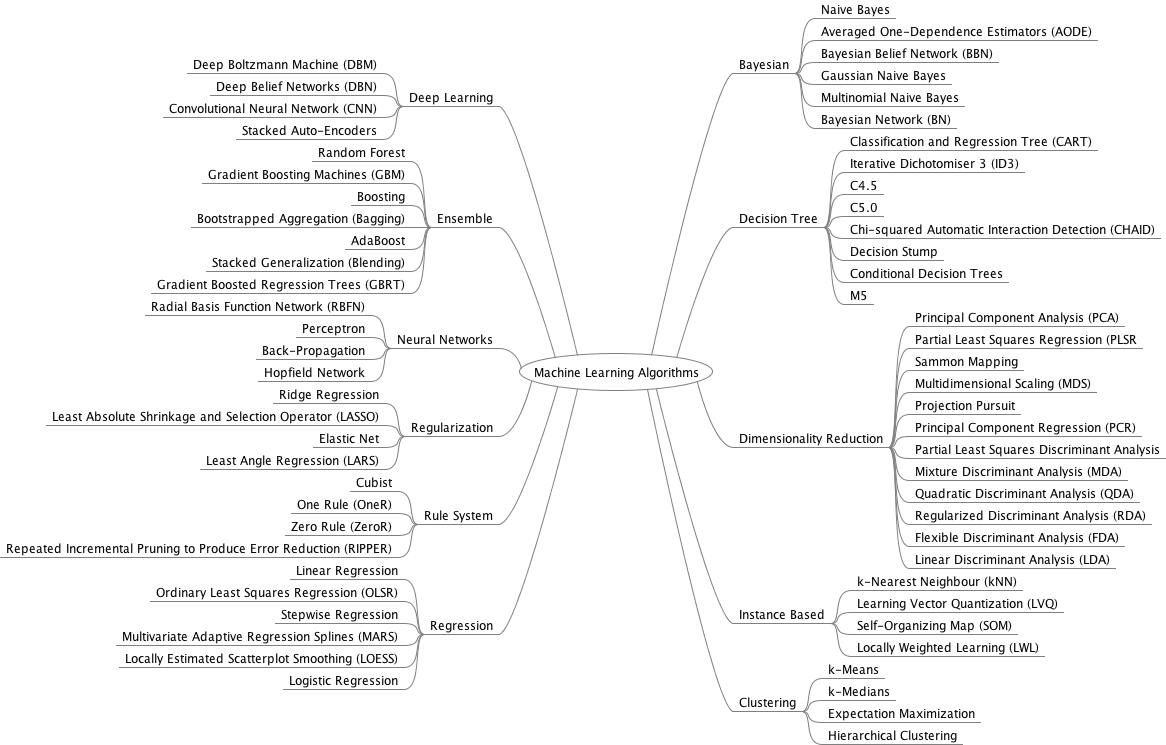
\includegraphics{mlalgs.png}
\caption{\textbf{Figure} :  Machine Learning Algorithms diagram from \href{http://machinelearningmastery.com/a-tour-of-machine-learning-algorithms/}{Jason Brownlee} .}\end{figure}
\end{quote}


\section{Categories of Data Mining Algorithms}
\label{algsummary:jason-brownlee}\label{algsummary:categories-of-data-mining-algorithms}\begin{enumerate}
\setcounter{enumi}{-1}
\item {} 
Dimensionality Reduction Algorithms

\end{enumerate}
\begin{itemize}
\item {} 
Principal Component Analysis (PCA)

\item {} 
Nonnegative Matrix Factorization (NMF)

\item {} 
Independent Component Analysis (ICA)

\item {} 
Linear Discriminant Analysis (LDA)

\end{itemize}
\begin{enumerate}
\item {} 
Regression Algorithms

\end{enumerate}
\begin{itemize}
\item {} 
Ordinary Least Squares Regression (OLSR)

\item {} 
Linear Regression

\item {} 
Logistic Regression

\end{itemize}
\begin{enumerate}
\setcounter{enumi}{1}
\item {} 
Regularization Algorithms

\end{enumerate}
\begin{itemize}
\item {} 
Ridge Regression

\item {} 
Least Absolute Shrinkage and Selection Operator (LASSO)

\item {} 
Elastic Net

\item {} 
Least-Angle Regression (LARS)

\end{itemize}
\begin{enumerate}
\setcounter{enumi}{2}
\item {} 
Decision Tree Algorithms

\end{enumerate}
\begin{itemize}
\item {} 
Classification and Regression Tree (CART)

\item {} 
Conditional Decision Trees

\end{itemize}
\begin{enumerate}
\setcounter{enumi}{4}
\item {} 
Bayesian Algorithms

\end{enumerate}
\begin{itemize}
\item {} 
Naive Bayes

\end{itemize}
\begin{enumerate}
\setcounter{enumi}{5}
\item {} 
Clustering Algorithms

\end{enumerate}
\begin{itemize}
\item {} 
k-Means

\item {} 
k-Medians

\item {} 
Expectation Maximisation (EM)

\item {} 
Hierarchical Clustering

\end{itemize}
\begin{enumerate}
\setcounter{enumi}{7}
\item {} 
Artificial Neural Network Algorithms

\end{enumerate}
\begin{itemize}
\item {} 
Perceptron

\item {} 
Back-Propagation

\item {} 
Hopfield Network

\item {} 
Radial Basis Function Network (RBFN)

\end{itemize}
\begin{enumerate}
\setcounter{enumi}{8}
\item {} 
Deep Learning Algorithms

\end{enumerate}
\begin{itemize}
\item {} 
Deep Boltzmann Machine (DBM)

\item {} 
Deep Belief Networks (DBN)

\end{itemize}
\begin{enumerate}
\setcounter{enumi}{10}
\item {} 
Ensemble Algorithms

\end{enumerate}
\begin{itemize}
\item {} 
Boosting

\item {} 
Bootstrapped Aggregation (Bagging)

\item {} 
AdaBoost

\item {} 
Gradient Boosting Machines (GBM)

\item {} 
Gradient Boosted Regression Trees (GBRT)

\item {} 
Random Forest

\end{itemize}
\phantomsection\label{dim:dim}
\index{Dimension Reduction Algorithms}

\chapter{Dimension Reduction Algorithms}
\label{dim:index-0}\label{dim::doc}\label{dim:dimension-reduction-algorithms}

\section{What is dimension reduction?}
\label{dim:what-is-dimension-reduction}
\textbf{In machine learning and statistics, dimensionality reduction or dimension reduction is the process of reducing the number of random variables under consideration,
via obtaining a set ``uncorrelated'' principle variables. It can be divided into feature selection and feature extraction.} \href{https://en.wikipedia.org/wiki/Dimensionality\_reduction}{https://en.wikipedia.org/wiki/Dimensionality\_reduction}

\index{Singular Value Decomposition}

\section{Singular Value Decomposition (SVD)}
\label{dim:index-1}\label{dim:singular-value-decomposition-svd}
At here, I will recall the three types of the SVD method, since some authors confused
the definitions of these SVD method. SVD method is important for the the dimension reduction
algorithms, such as Truncated Singular Value Decomposition (tSVD) can be used to do the dimension
reduction directly, and the Full Rank Singular Value Decomposition (SVD) can be applied to do Principal Component Analysis (PCA), since PCA is a specific case of SVD.
\begin{enumerate}
\item {} 
\textbf{Full Rank Singular Value Decomposition (SVD)}

\end{enumerate}
\begin{quote}

Suppose \({\bf X}\in\mathbb{R}^{n\times p}, (p<n)\), then
\phantomsection\label{dim:equation-svd}\begin{gather}
\begin{split}    \underbracket{\bf X}_{n\times p} =\underbracket{\bf U}_{n\times n} \underbracket{\bf\Sigma}_{n\times p} \underbracket{{\bf V}^T}_{p\times p},\end{split}\label{dim-svd}
\end{gather}
is called a full rank \textbf{SVD} of \({\bf X}\) and
\begin{itemize}
\item {} 
\(\sigma_i\)-- Sigular calues and \({\bf\Sigma}=diag(\sigma_1,\sigma_2, \cdots, \sigma_p)\in \mathbb{R}^{n\times p}\)

\item {} 
\(u_i\)-- left singular vectors, \({\bf U}=[u_1,u_2, \cdots, u_n]\) and  \({\bf U}\) is unitary.

\item {} 
\(v_i\)-- right singular vectors, \({\bf V}=[v_1,v_2, \cdots, v_p]\) and  \({\bf V}\) is unitary.

\end{itemize}
\begin{quote}
\begin{figure}[htbp]
\centering
\capstart

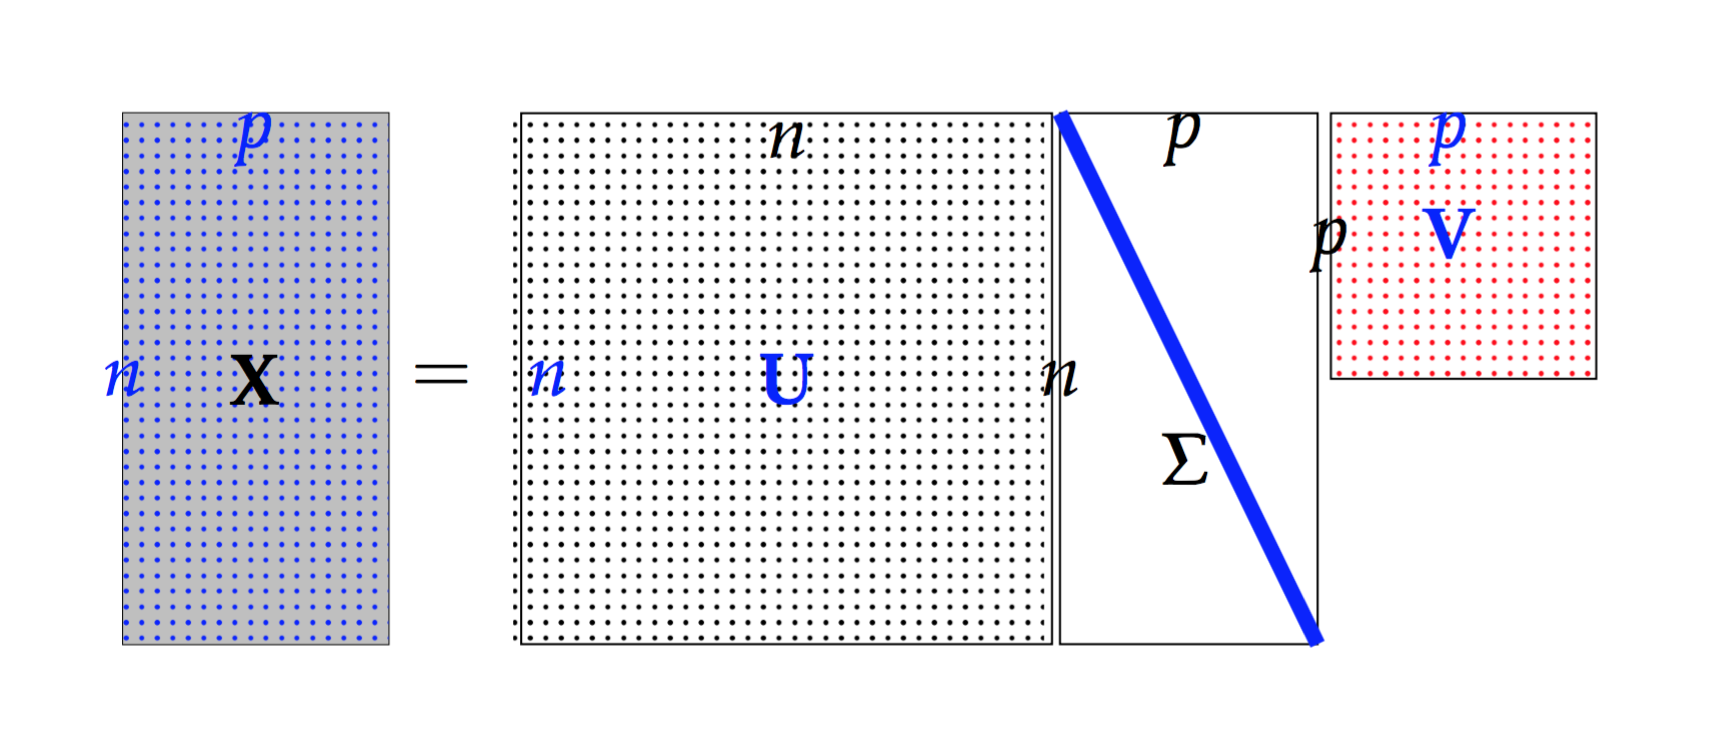
\includegraphics{svd.png}
\caption{Singular Value Decomposition}\label{dim:fig-svd}\end{figure}
\end{quote}
\end{quote}
\begin{enumerate}
\setcounter{enumi}{1}
\item {} 
\textbf{Reduced Singular Value Decomposition (rSVD)}

\end{enumerate}
\begin{quote}

Suppose \({\bf X}\in\mathbb{R}^{n\times p},(n<p)\), then
\phantomsection\label{dim:equation-rsvd}\begin{gather}
\begin{split}    \underbracket{\bf X}_{n\times p} =\underbracket{\bf \hat{U}}_{n\times p} \underbracket{\bf\hat{\Sigma}}_{p\times p} \underbracket{{\bf \hat{V}}^T}_{p\times p},\end{split}\label{dim-rsvd}
\end{gather}
is called a Reduced Singular Value Decomposition \textbf{rSVD} of \({\bX}\) and
\begin{itemize}
\item {} 
\(\sigma_i\)-- Sigular calues and \({\bf\hat{\Sigma}}=diag(\sigma_1,\sigma_2, \cdots, \sigma_p)\in \mathbb{R}^{p\times p}\)

\item {} 
\(u_i\)-- left singular vectors, \({\bf \hat{U}}=[u_1,u_2, \cdots, u_p]\) is column-orthonormal matrix.

\item {} 
\(v_i\)-- right singular vectors, \({\bf \hat{V}}=[v_1,v_2, \cdots, v_p]\) is column-orthonormal matrix.

\end{itemize}
\end{quote}
\begin{enumerate}
\setcounter{enumi}{2}
\item {} 
\textbf{Truncated Singular Value Decomposition (tSVD)}

\end{enumerate}
\begin{quote}

Suppose \({\bf X}\in\mathbb{R}^{n\times p},(r<p)\), then
\phantomsection\label{dim:equation-tsvd}\begin{gather}
\begin{split}    \underbracket{\bf X}_{n\times p} =\underbracket{\bf \hat{U}}_{n\times r} \underbracket{\bf\hat{\Sigma}}_{r\times r} \underbracket{{\bf \hat{V}}^T}_{r\times p},\end{split}\label{dim-tsvd}
\end{gather}
is called a Truncated Singular Value Decomposition \textbf{tSVD} of \({\bf X}\) and
\begin{itemize}
\item {} 
\(\sigma_i\)-- Sigular calues and \({\bf\hat{\Sigma}}=diag(\sigma_1,\sigma_2, \cdots, \sigma_r)\in \mathbb{R}^{r\times r}\)

\item {} 
\(u_i\)-- left singular vectors, \({\bf \hat{U}}=[u_1,u_2, \cdots, u_r]\) is column-orthonormal matrix.

\item {} 
\(v_i\)-- right singular vectors, \({\bf \hat{V}}=[v_1,v_2, \cdots, v_p]\) is column-orthonormal matrix.

\end{itemize}
\begin{quote}
\begin{figure}[htbp]
\centering
\capstart

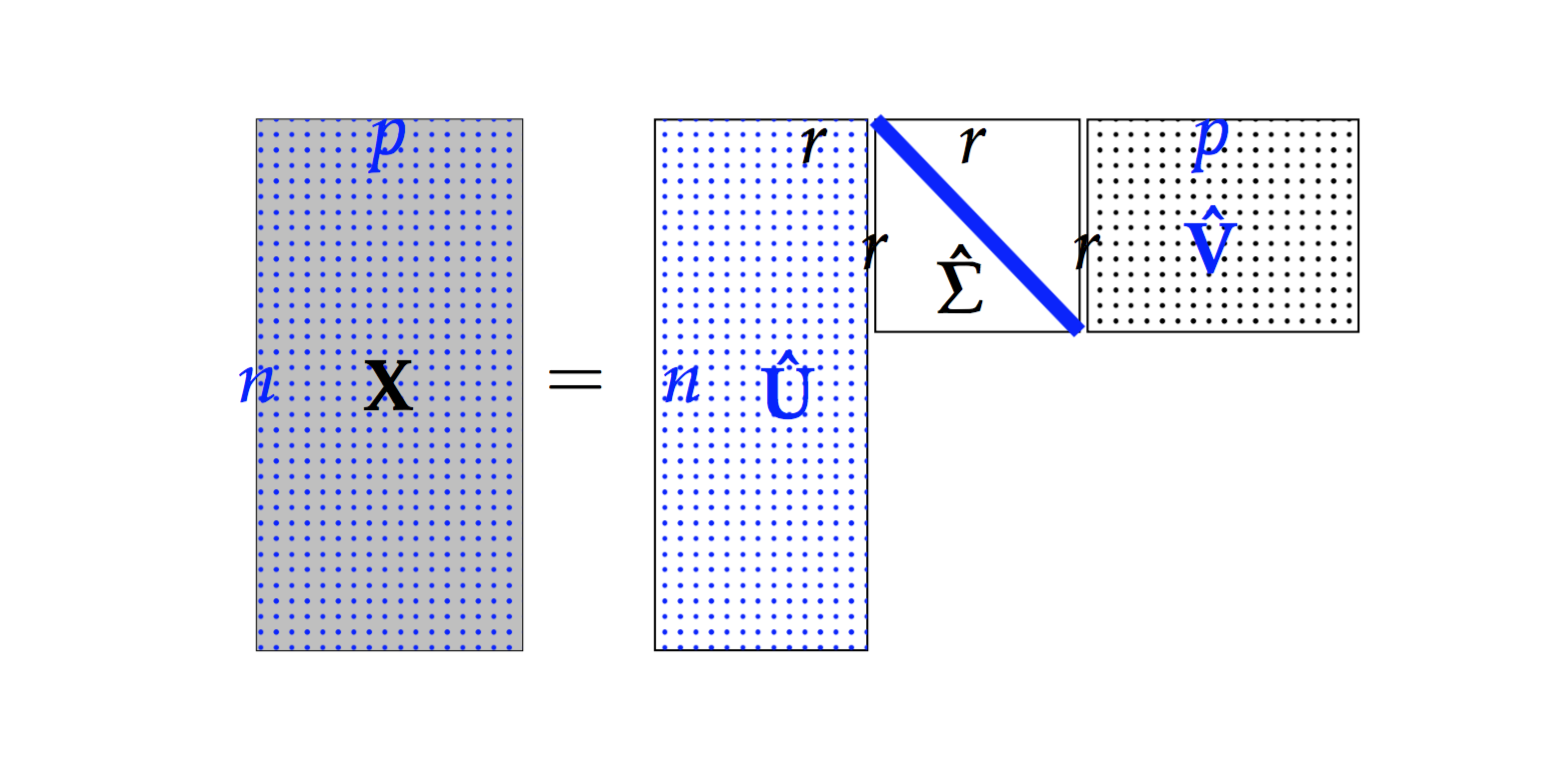
\includegraphics{tsvd.png}
\caption{Truncated Singular Value Decomposition}\label{dim:fig-tsvd}\end{figure}
\end{quote}
\end{quote}

Figure {\hyperref[dim:fig-tsvd]{\emph{Truncated Singular Value Decomposition}}} indictes that the the dimension of \({\bf \hat{U}}\) is smaller than \({\bf X}\). We can use this property to do the dimension reduction. But, usually, we will use SVD
to compute the Principal Components. We will learn more details in next section.

\index{Principal Component Analysis}

\section{Principal Component Analysis (PCA)}
\label{dim:principal-component-analysis-pca}\label{dim:index-2}
Principal Component Analysis (PCA) is a specific case of SVD.
\begin{quote}
\phantomsection\label{dim:equation-test}\begin{gather}
\begin{split}\underbracket{\bX}_{n\times p} =\hU\end{split}\label{dim-test}
\end{gather}\end{quote}

\index{Independent Component Analysis}

\section{Independent Component Analysis (ICA)}
\label{dim:independent-component-analysis-ica}\label{dim:index-3}
\index{Nonnegative matrix factorization}

\section{Nonnegative matrix factorization (NMF)}
\label{dim:index-4}\label{dim:nonnegative-matrix-factorization-nmf}
TO DO......


\chapter{Regression Algorithm}
\label{regression:regression-algorithm}\label{regression::doc}\label{regression:regression}

\section{Ordinary Least Squares Regression (OLSR)}
\label{regression:ordinary-least-squares-regression-olsr}

\section{Linear Regression (LR)}
\label{regression:linear-regression-lr}

\section{Logistic Regression (logR)}
\label{regression:logistic-regression-logr}
TO DO .....


\chapter{Classification ALgorithms}
\label{classification::doc}\label{classification:classification-algorithms}\label{classification:classification}

\section{Logistic Regression (LR)}
\label{classification:logistic-regression-lr}

\section{k-Nearest Neighbour (kNN)}
\label{classification:k-nearest-neighbour-knn}

\section{Linear Discriminant Analysis (LDA)}
\label{classification:linear-discriminant-analysis-lda}

\section{Quadratic Discriminant Analysis (QDA)}
\label{classification:quadratic-discriminant-analysis-qda}
TO DO .....


\chapter{Regularization ALgorithms}
\label{reg:regularization-algorithms}\label{reg::doc}\label{reg:reg}

\section{Subset Selection (SubS)}
\label{reg:subset-selection-subs}

\section{Ridge Regression (Ridge)}
\label{reg:ridge-regression-ridge}

\section{Least Absolute Shrinkage and Selection Operator (lASSO)}
\label{reg:least-absolute-shrinkage-and-selection-operator-lasso}
TO DO .....


\chapter{Resampling Algorithms}
\label{resample:resample}\label{resample::doc}\label{resample:resampling-algorithms}
TO DO .....


\chapter{Developing Your Own R Packages}
\label{rpkg:rpkg}\label{rpkg::doc}\label{rpkg:developing-your-own-r-packages}
TO DO......


\chapter{Developing Your Own Python Packages}
\label{ppkg:developing-your-own-python-packages}\label{ppkg:ppkg}\label{ppkg::doc}
TO DO......



\renewcommand{\indexname}{Index}
\printindex
\end{document}
